\section{Chapter 3}
\section{-----temp move-----}

\subsection{Degree and orthologs}

If the network is generated by the preferential attachment model of Barabasi we would expect the nodes of high degree to have more ancient orthologues than those of lower degree.  Duplication divergence \todo{ref} may be an important mechanism as we know there was a genome duplication event nevertheless we could hypothesise that the nodes with yeast orthologues will have higher median degree than the human and murine PSP. \todo{add cross ref to orthologues}
\subsection{Results of disease enrichment for centrality measures}
\label{sec:disgennet2r tables}
Using the package disgennet2r disease enrichment was performed using the curated disgennet database using fishers exact test with FDR correction for multiple comparisons. 9703 genes were used as the background being those genes with annotated disease associations (not specifically synaptic)
\subsubsection{Degree}

Low degree (bottom 10\%) ataxia and seizures cut off 0.05

\begin{figure}
    \centering
    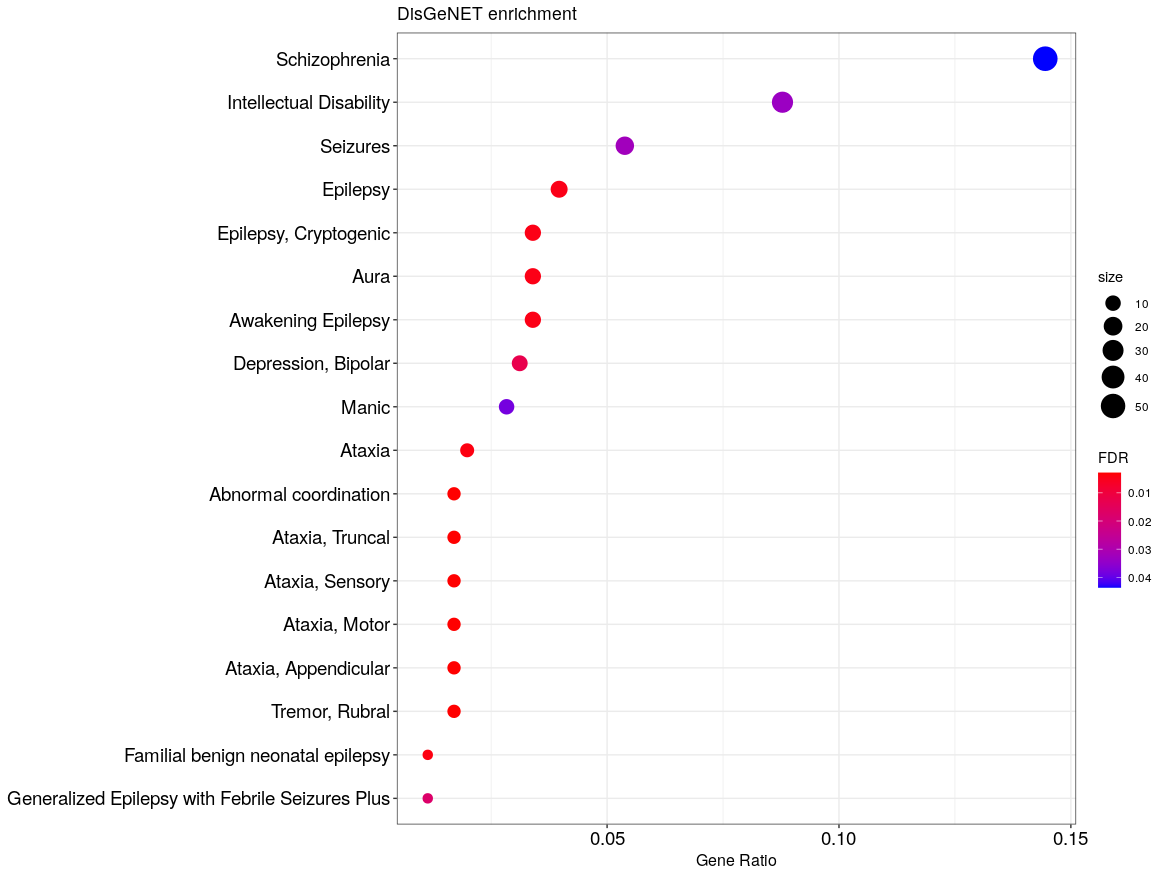
\includegraphics[width=\textwidth]{images/Rplot_low_deg_0point05cutoff_0point1cent_disgen.png}
    \caption{Low degree disease enrichment}
    \label{fig:low degree disease enrichment cut off 0.05}
\end{figure}


\begin{figure}
    \centering
    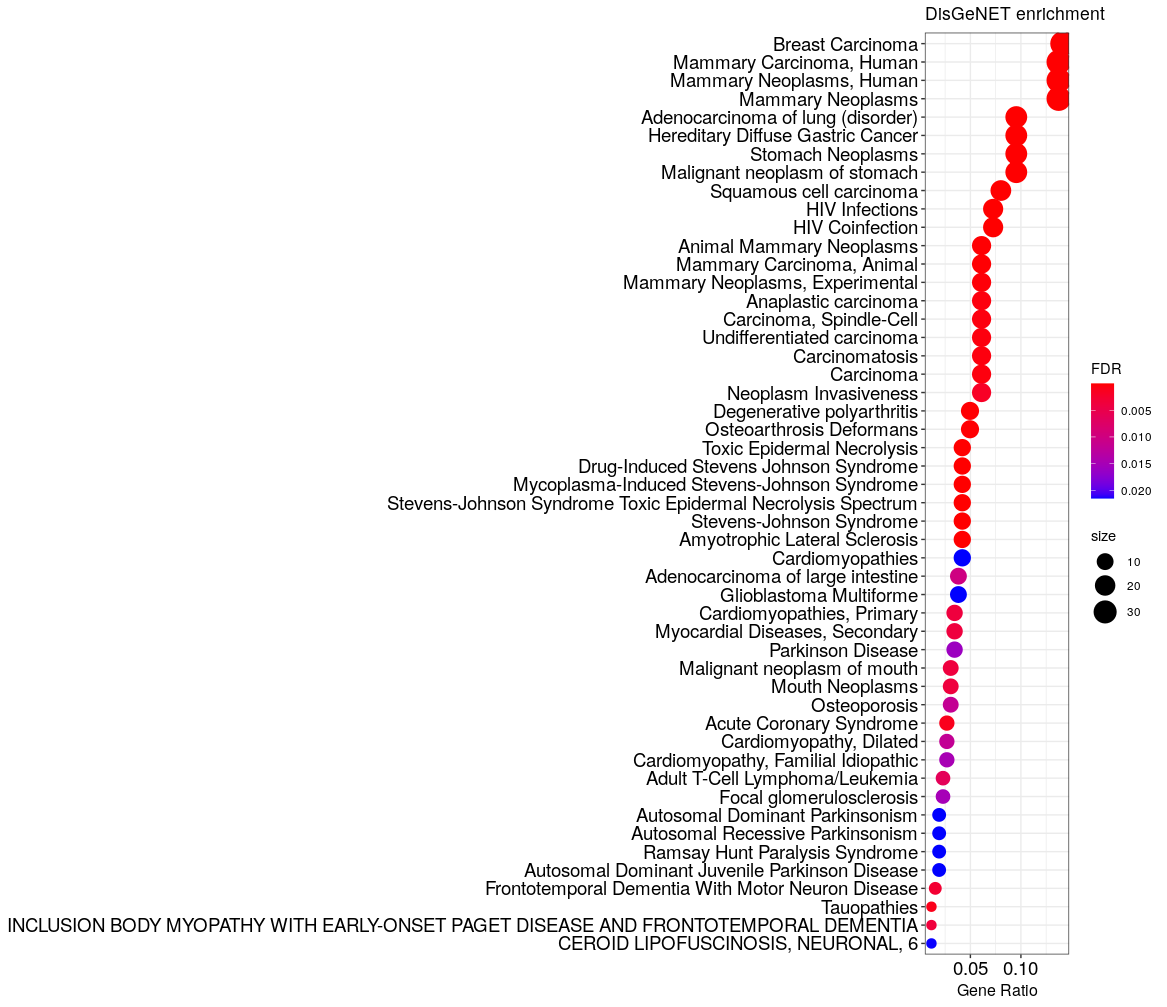
\includegraphics[width=\textwidth]{images/Rplot_high_deg_0point9_0point05cutoff_disgen.png}
    \caption{High degree disease enrichment}
    \label{fig:High degree disease enrichment cut off 0.05}
\end{figure}
Low degree includes a number of epilepsy (figure~\ref{fig:low degree disease enrichment cut off 0.05}). High degree (greater than 0.9 centile) enriches for neurological conditions ALS and Parkinson's disease (figure~\ref{fig:low degree disease enrichment cut off 0.05}).


Code \url{source('~/RProjects/graph2community/R/disgen3_degree_hi.R')}
\subsubsection{betweennness}



Diseases associated with high betweenness centrality were predominantly neoplasms showing those above the 90th centile for betweenness 0.0001121076, those in the bottom 10\% ($8.3 \times 10^{-5}$) were predominantly neurological disorders.

This suggests that highly central nodes are either not compatible with viability or are only affected in severely disordered pathology affecting essential cell functions such as tumours. 



\begin{figure}
    \centering
    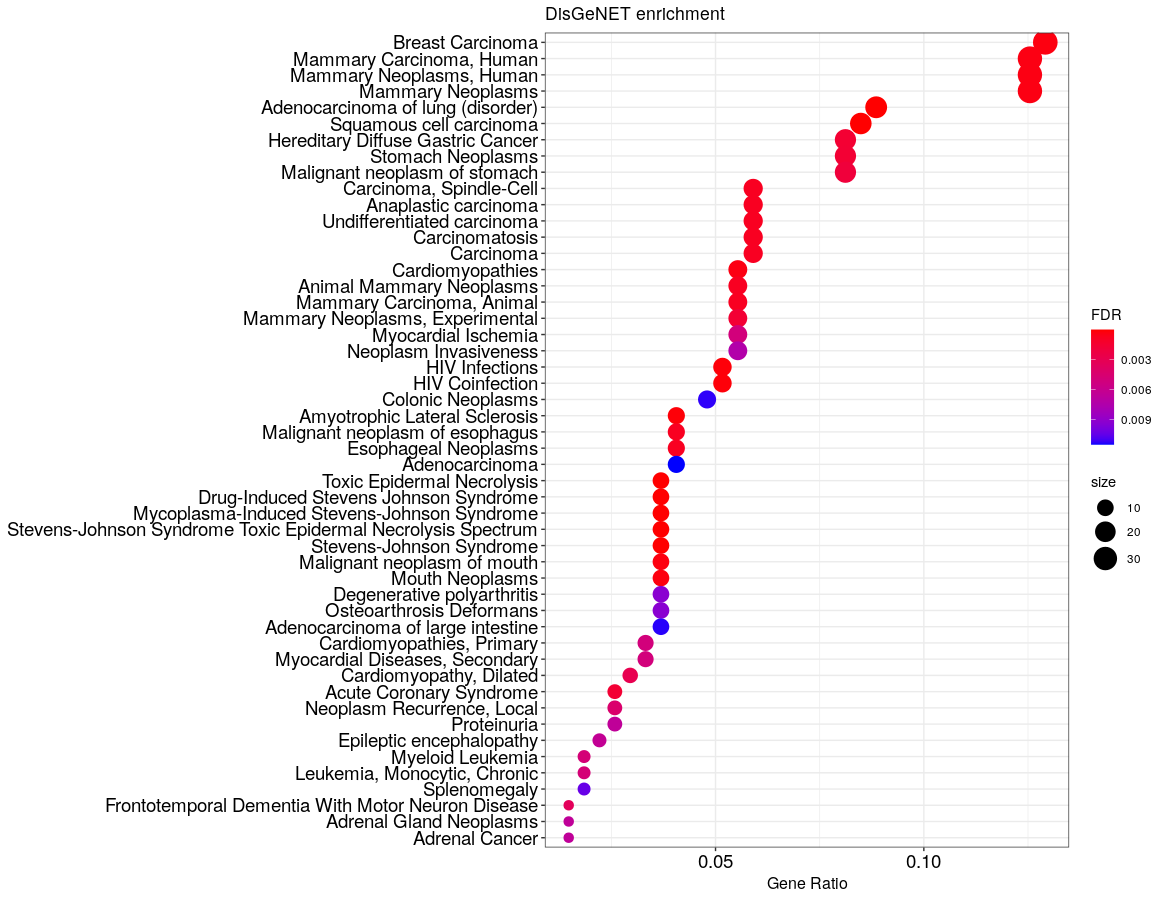
\includegraphics[width=\textwidth]{images/Rplot_high_bet_disgen.png}
    \caption{High betweenness nodes disease enrichment}
    \label{fig:high betweenness disease enrichment}
\end{figure}

\begin{figure}
    \centering
    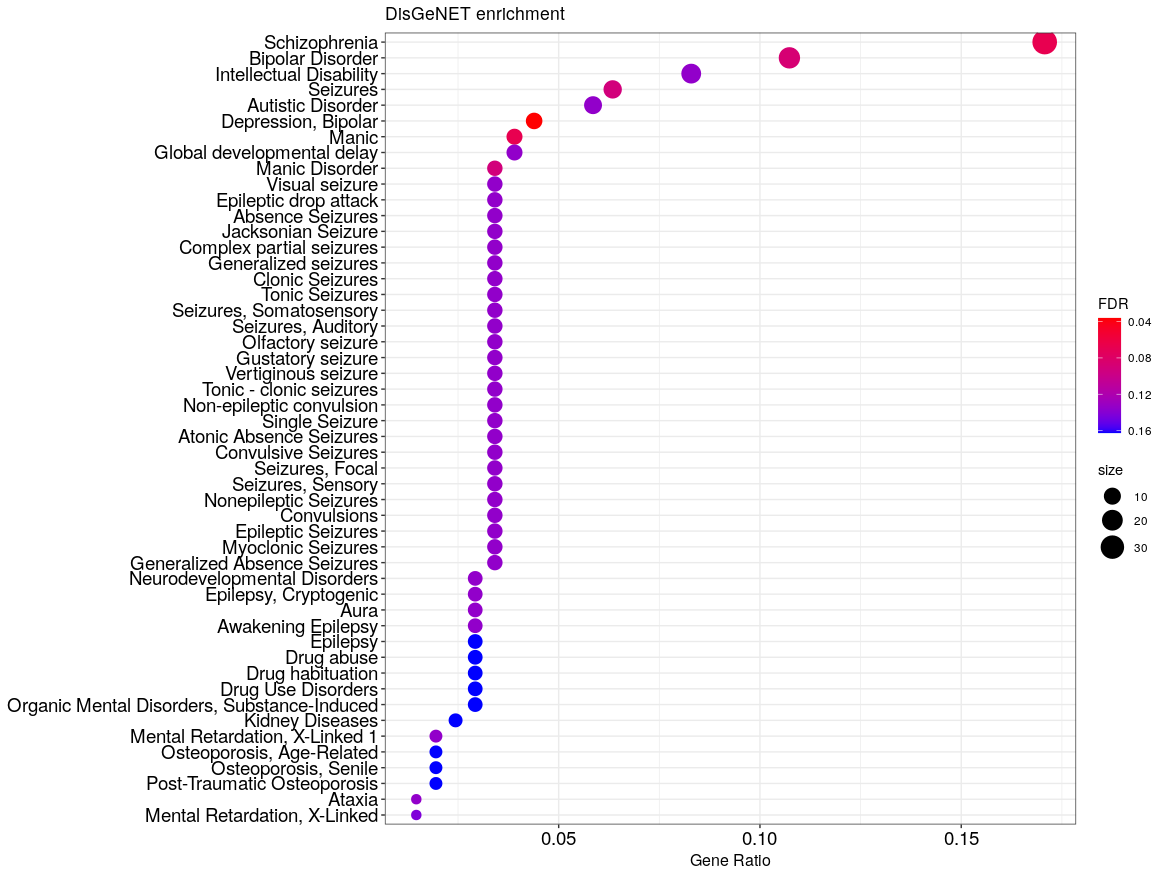
\includegraphics[width=\textwidth]{images/Rplot_bet_low0point1point.png}
    \caption{Low betweenness disease enrichment}
    \label{fig:low betweenness disease enrichment}
\end{figure}



\subsubsection{Closeness centrality}



\begin{figure}
    \centering
    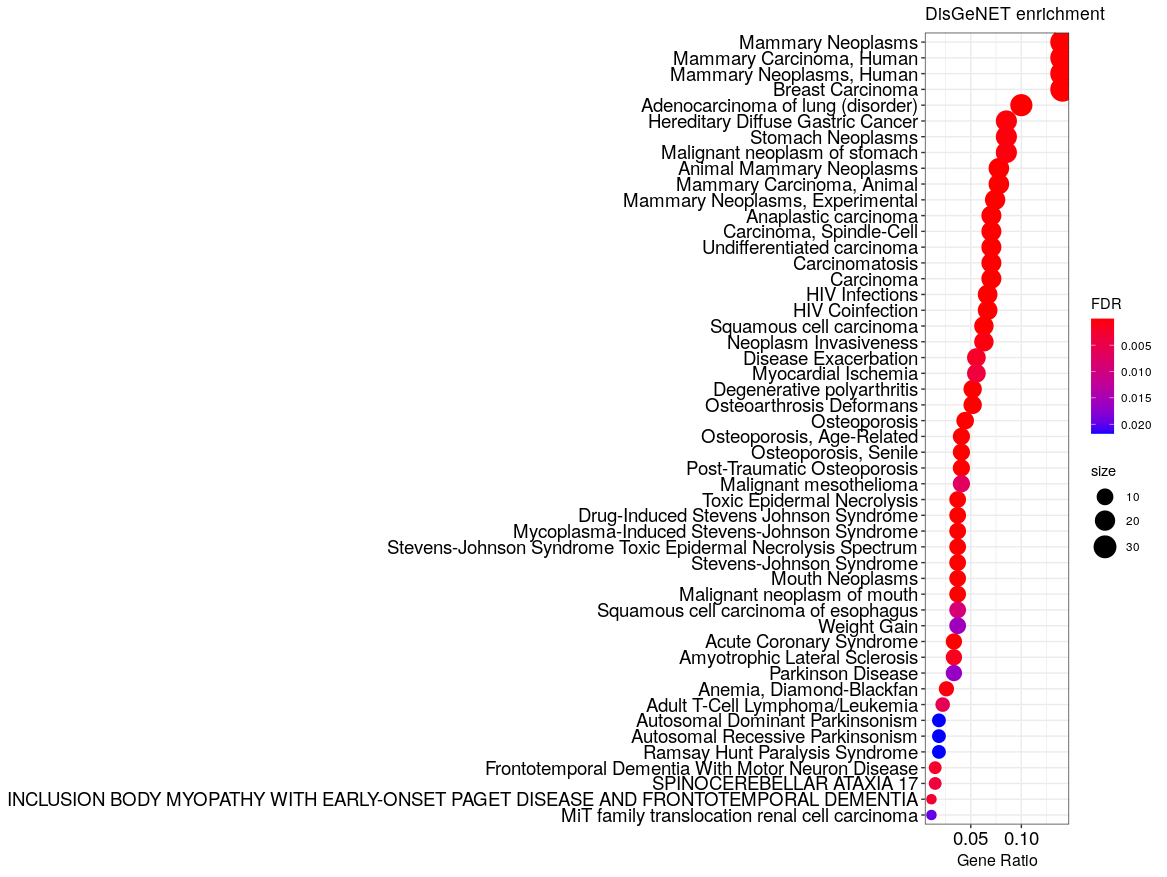
\includegraphics[width=\textwidth]{images/Rplot_high_closeness.png}
    \caption{High closeness disease enrichment}
    \label{fig:high closeness disease enrichment}
\end{figure}

\begin{figure}
    \centering
    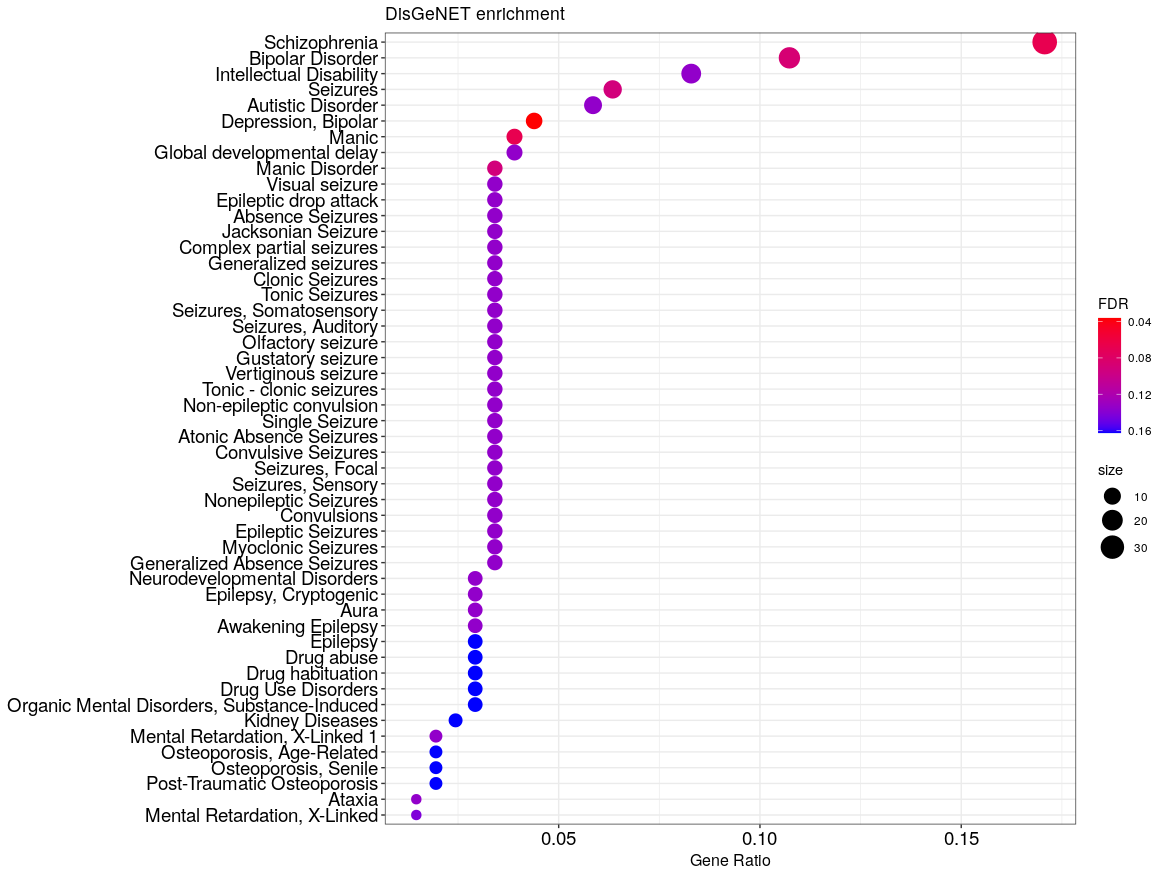
\includegraphics[width=\textwidth]{images/Rplot_low_closeness.png}
    \caption{Low closeness disease enrichment}
    \label{fig:low closeness disease enrichment}
\end{figure}



Note that the neurological conditions that are present with high closeness centrality are parkinsonism and some neurodegeneration


\subsubsection{Eigenvector centrality}

Parkinsons disease is again the highest ranking neurological disease in high eirgenvector centrality enrichment

40 low eigenvector annotated (greater than 0.9 centile)

261 high eigenvector centrality annotated (less than 0.1)


DisGeNet Low eigenvector centrality (figure~\ref{fig:low eigenvector disease enrichment cut off 0.05}.

Gene Ratio is number of terms from gene set in annotation over size of annotation

\begin{figure}
    \centering
    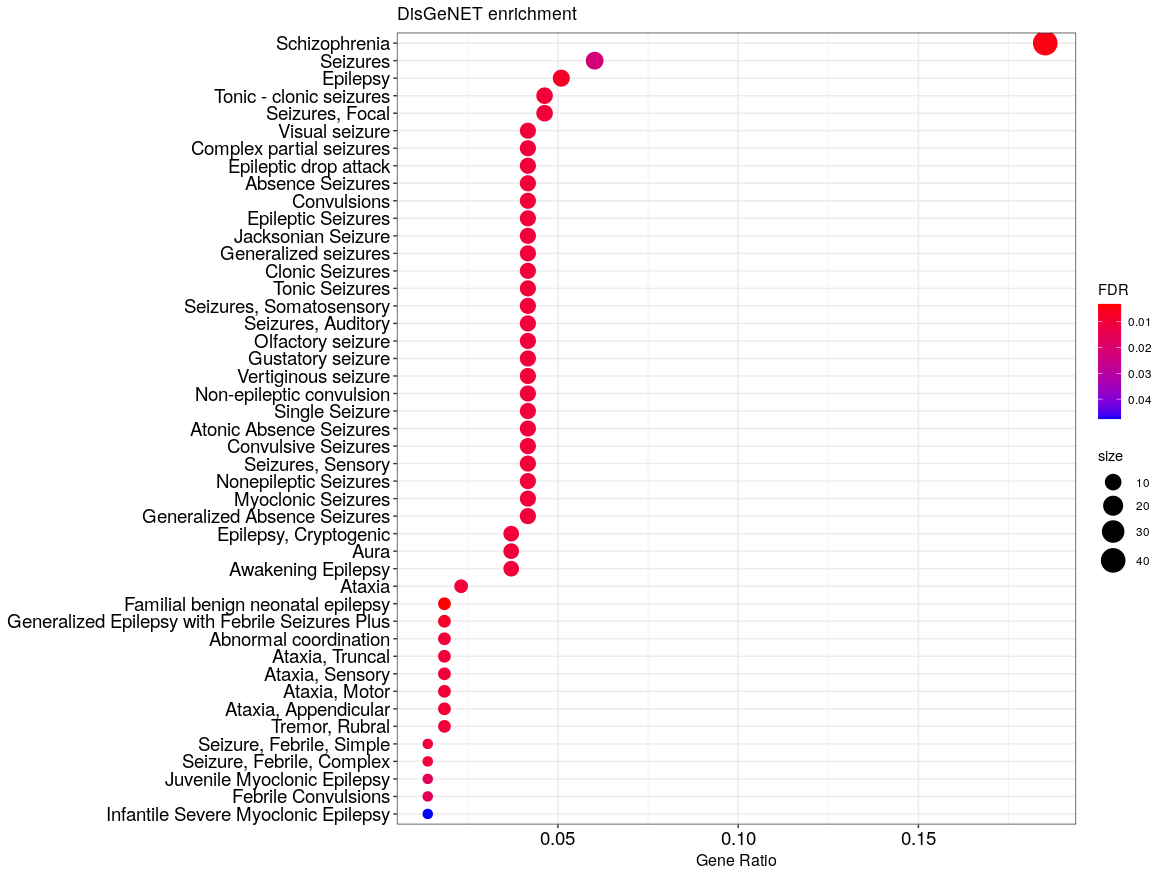
\includegraphics[width=\textwidth]{images/Rplot_low_eigenvector_centrality.png}
    \caption{Low eigenvector disease enrichment}
    \label{fig:low eigenvector disease enrichment cut off 0.05}
\end{figure}


\begin{figure}
    \centering
    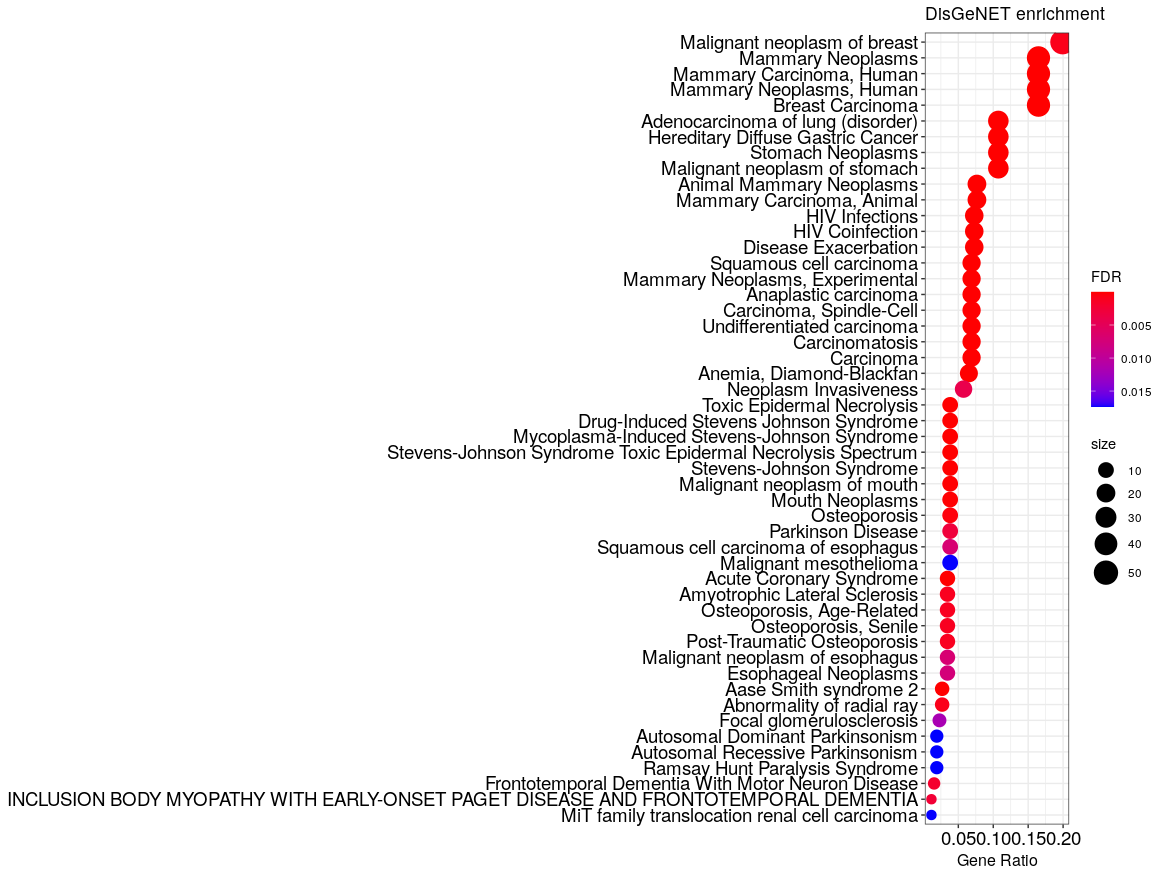
\includegraphics[width=\textwidth]{images/Rplot_high_eigenvector_centrality_disggen0point9.png}
    \caption{High eigenvector disease enrichment}
    \label{fig:high eigenvector disease enrichment cut off 0.05}
\end{figure}


\subsubsection{Further notes on disease enrichment}
Should do ID as related to cognition

\subsubsection{Disgenet}
\paragraph{Betweenness}
Betweenness flat at 0 to 10\% (low)

In disgennet point at 97.5\% where neurological conditions come to fore.
\paragraph{Eigenvector}
\subparagraph{High}
\url{source('~/RProjects/disgen2/R/disgen/background_ents/enrich_bg_high_and_low.R')}
35 genes 1\%
Number 3+1 disease is ALS 354 genes in synapse
1069 genes

FTD with MND 3 of 5 genes
GRN related FTD 6 of 47
ft lobar 7 of 81

97.5\%
87 genes

ALS 15 C0002736 Be Free 29 of 354
Alz Familial 24 C1843013 11 of 57
PD 32 C0030567 34 of 548 
Neurodegenerative  46 C0524851 31 of 484
Frontotemporal frontolobar 47 C0751072 12 of 81


95\%
173 genes

C is UMLS CUI: 
FTD 3 C0338451 27 of 119
ALS 4 C0002736 48 of 354
Japanese enceph 25
Picks 27 C0236642 20 of 89
Frontotemporal lobar C0751072 19 of 81
GRN related FTD C3811918 14 of 47


\subparagraph{Low}
Bottom 1\% neuro conditions on disgen 35 genes
No disease on ToppGene
 \section{---Move to other chapters---}
 \subsection{From the biomedical centrality measures bit to go to community detection}
 \textcolor{red}{this is really a paper where they get gene level scores and then find a module that has maximal association with the phenotype. They do this using cut methods so this probably belongs in the community detection section. The reason this is different is that they use a heterogenous network (gene interactions, PPI etc) and somewhat arbitrary edge weights which is an approach we have already rejected in the introduction when talking about only using high quality interaction data but it is faily similar to our approach}
Liu \cite{liu2017sigmod} described a method of identifying gene modules and combining this with p values but use heterogenous different measures of gene interaction including coexpression from the STRING database version 10 which results in what they refer to as a GeneNet \todo{there is a thing called a gene net - check} with 19 247 genes and 4 274 001 edges. Edges are given weights based on level of evidence but if there is a connection but no weighting a value of 1 is given. Nodes are given higher significance based on degree.  Gene level P values were obtained by calculating the value of the top SNP within a gene. They compare their results to two other methods dmGWAS and SCoNEs. Their method is implemented in an R module (SigMod) last updated 2 years ago \todo{remove this this is to jog my memory}. They appear to use a min cut algorithm to find modules and take into account degree. THere is also a complex method for adjusting two tunable parameters \todo{can't really make head or tail of this paper. Don't know why they didn't use something like VEGAS. }\textcolor{red}{end}

\section{General to dos}

Table of diameters \cite{crescenzi2013computing}
 table 4 
 \todo{enrichment of high/low scoring groups of genes}
 \todo{add intellectual disability graph measures or indeed other disorders from ToppGene}
 \todo{define configuration model}
 \todo{plot of distribution of other centrality measures}
\todo{centrality measures for significant genes}
\todo{centralisation 1:09 in zhukov - centrality is how central most central node is compared to other nodes in graph, max with star network}
\todo{Metrics comparison zhukov at 1:15}
%Scatter plot of centralities multiplot eg plot(bet,deg) DONE

Kendal tau rank - concordant pairs ie a comes before b in both samples 

most recent centrality in \url{source('~/RProjects/centrality/R/other_centrality/eccentricity_and_distance.R')}


\section{Value of tissue specific networks}
\cite{parikshak2015systems} quotes the example of cardiac PPI to investigaste long QT in \cite{lundby2014annotation}

Kitsak and Barabasi \cite{kitsak2016tissue}

\section{This chapter extra refs}

@misc{vespignani2018twenty,
  title={Twenty years of network science},
  author={Vespignani, Alessandro},
  year={2018},
  publisher={Nature Publishing Group}
}

@article{barbey2018network,
  title={Network neuroscience theory of human intelligence},
  author={Barbey, Aron K},
  journal={Trends in cognitive sciences},
  volume={22},
  number={1},
  pages={8--20},
  year={2018},
  publisher={Elsevier}
}


\section{this chapter supplementary tables}
\subsubsection{High degree}
\paragraph{Human phenotype}

% latex table generated in R 3.6.3 by xtable 1.8-4 package
% Sun Oct  4 15:35:31 2020
\begin{table}[ht]
\centering
\begin{adjustbox}{width=\textwidth}
\begin{tabular}{llrrrr}
  \hline
ID & Human Phenotype & n & n PSP & p & q FDR B H \\ 
  \hline
HP:0002664 & Neoplasm & 50 & 267 & $4.65 \times 10^{-6}$ & $1.12 \times 10^{-2}$ \\ 
  HP:0002145 & Frontotemporal dementia & 13 & 32 & $8.66 \times 10^{-6}$ & $1.12 \times 10^{-2}$ \\ 
  HP:0011793 & Neoplasm by anatomical site & 48 & 262 & $1.65 \times 10^{-5}$ & $1.12 \times 10^{-2}$ \\ 
  HP:0007024 & Pseudobulbar paralysis & 11 & 25 & $1.83 \times 10^{-5}$ & $1.12 \times 10^{-2}$ \\ 
  HP:0100242 & Sarcoma & 25 & 101 & $2.11 \times 10^{-5}$ & $1.12 \times 10^{-2}$ \\ 
  HP:0002200 & Pseudobulbar signs & 12 & 30 & $2.40 \times 10^{-5}$ & $1.12 \times 10^{-2}$ \\ 
  HP:0011844 & Abnormal appendicular skeleton morphology & 70 & 450 & $2.49 \times 10^{-5}$ & $1.12 \times 10^{-2}$ \\ 
  HP:0100851 & Abnormal emotion/affect behavior & 49 & 274 & $2.65 \times 10^{-5}$ & $1.12 \times 10^{-2}$ \\ 
  HP:0003006 & Neuroblastoma & 18 & 62 & $3.69 \times 10^{-5}$ & $1.12 \times 10^{-2}$ \\ 
  HP:0030067 & Peripheral primitive neuroectodermal neoplasm & 18 & 62 & $3.69 \times 10^{-5}$ & $1.12 \times 10^{-2}$ \\ 
   \hline
\end{tabular}
\end{adjustbox}
\caption{ToppGene Human Phenotype. 90 centile cwpsp.txtp = p value; q FDR B H = q adjusted significance level False Discovery Rate using Benjamini and Hochberg adjustment; n= n genes annotated in test group; n PSP= n genes annotated in PSP. n significant in category 131} 
\label{tab:ToppGENE Human Phenotype. 90 centile cwpsp.txtp = p value; q FDR B H = q adjusted significance level False Discovery Rate using Benjamini and Hochberg adjustment; n= n genes annotated in test group; n PSP= n genes annotated in PSP. n significant in category 131}
\end{table}
% latex table generated in R 3.6.3 by xtable 1.8-4 package
% Sun Oct  4 11:53:35 2020
\begin{table}[ht]
\centering
\begin{adjustbox}{width=\textwidth}
\begin{tabular}{llrrrr}
  \hline
ID & Disease & n & n PSP & p & q FDR B H \\ 
  \hline
C0042769 & Virus Diseases & 93 & 332 & $6.39 \times 10^{-22}$ & $5.53 \times 10^{-18}$ \\ 
  C0019163 & Hepatitis B & 84 & 290 & $1.01 \times 10^{-20}$ & $4.36 \times 10^{-17}$ \\ 
  C2931822 & Nasopharyngeal carcinoma & 82 & 294 & $4.76 \times 10^{-19}$ & $1.37 \times 10^{-15}$ \\ 
  C1332977 & Childhood Leukemia & 90 & 367 & $6.78 \times 10^{-17}$ & $1.47 \times 10^{-13}$ \\ 
  C0040136 & Thyroid Neoplasm & 67 & 231 & $1.84 \times 10^{-16}$ & $3.11 \times 10^{-13}$ \\ 
  C0026764 & Multiple Myeloma & 85 & 341 & $2.22 \times 10^{-16}$ & $3.11 \times 10^{-13}$ \\ 
  C0023418 & leukemia & 95 & 407 & $2.51 \times 10^{-16}$ & $3.11 \times 10^{-13}$ \\ 
  C0029408 & Degenerative polyarthritis & 76 & 293 & $1.24 \times 10^{-15}$ & $1.34 \times 10^{-12}$ \\ 
  C0024299 & Lymphoma & 77 & 300 & $1.46 \times 10^{-15}$ & $1.40 \times 10^{-12}$ \\ 
  C1832661 & ANOPHTHALMIA AND PULMONARY HYPOPLASIA & 76 & 298 & $3.45 \times 10^{-15}$ & $2.99 \times 10^{-12}$ \\ 
  C0030567 & Parkinson Disease & 111 & 548 & $2.23 \times 10^{-14}$ & $1.75 \times 10^{-11}$ \\ 
  C0007134 & Renal Cell Carcinoma & 92 & 415 & $2.99 \times 10^{-14}$ & $2.16 \times 10^{-11}$ \\ 
  C0546837 & Malignant neoplasm of esophagus & 65 & 242 & $3.69 \times 10^{-14}$ & $2.45 \times 10^{-11}$ \\ 
  C3539878 & Triple Negative Breast Neoplasms & 82 & 351 & $5.21 \times 10^{-14}$ & $3.22 \times 10^{-11}$ \\ 
  C0033578 & Prostatic Neoplasms & 53 & 175 & $6.05 \times 10^{-14}$ & $3.49 \times 10^{-11}$ \\ 
  C0002736 & Amyotrophic Lateral Sclerosis & 82 & 354 & $8.76 \times 10^{-14}$ & $4.39 \times 10^{-11}$ \\ 
  C0549473 & Thyroid carcinoma & 64 & 240 & $8.79 \times 10^{-14}$ & $4.39 \times 10^{-11}$ \\ 
  C0007847 & Malignant tumor of cervix & 76 & 315 & $9.14 \times 10^{-14}$ & $4.39 \times 10^{-11}$ \\ 
  C0677886 & Epithelial ovarian cancer & 62 & 230 & $1.35 \times 10^{-13}$ & $5.85 \times 10^{-11}$ \\ 
  C0007115 & Malignant neoplasm of thyroid & 56 & 195 & $1.35 \times 10^{-13}$ & $5.85 \times 10^{-11}$ \\ 
   \hline
\end{tabular}
\end{adjustbox}
\caption{ToppGene Disease. bet 90 centile cwpsp.txtp = p value; q FDR B H = q adjusted significance level False Discovery Rate using Benjamini and Hochberg adjustment; n= n genes annotated in test group; n PSP= n genes annotated in PSP} 
\label{tab:ToppGENE Disease. bet 90 centile cwpsp.txtp = p value; q FDR B H = q adjusted significance level False Discovery Rate using Benjamini and Hochberg adjustment; n= n genes annotated in test group; n PSP= n genes annotated in PSP}
\end{table}

\paragraph{Closeness centrality Low}
\subparagraph{Human phenotype}
% latex table generated in R 3.6.3 by xtable 1.8-4 package
% Sun Oct  4 12:27:26 2020
\begin{table}[ht]
\centering
\begin{tabular}{llrrrr}
  \hline
ID & Human Phenotype & n & n PSP & p & q FDR B H \\ 
  \hline
HP:0002123 & Generalized myoclonic seizure & 12 & 28 & $3.23 \times 10^{-6}$ & $9.13 \times 10^{-3}$ \\ 
  HP:0002121 & Generalized non-motor (absence) seizure & 11 & 28 & $2.36 \times 10^{-5}$ & $2.78 \times 10^{-2}$ \\ 
  HP:0011146 & Dialeptic seizure & 12 & 34 & $3.50 \times 10^{-5}$ & $2.78 \times 10^{-2}$ \\ 
  HP:0011153 & Focal motor seizure & 8 & 16 & $4.18 \times 10^{-5}$ & $2.78 \times 10^{-2}$ \\ 
  HP:0007334 & Bilateral tonic-clonic seizure with focal onset & 6 & 9 & $4.92 \times 10^{-5}$ & $2.78 \times 10^{-2}$ \\ 
   \hline
\end{tabular}
\caption{ToppGene Human Phenotype. clo 10 centile cwpsp.txtp = p value; q FDR B H = q adjusted significance level False Discovery Rate using Benjamini and Hochberg adjustment; n= n genes annotated in test group; n PSP= n genes annotated in PSP} 
\label{tab:ToppGENE Human Phenotype. clo 10 centile cwpsp.txtp = p value; q FDR B H = q adjusted significance level False Discovery Rate using Benjamini and Hochberg adjustment; n= n genes annotated in test group; n PSP= n genes annotated in PSP}
\end{table}
\subparagraph{Disease topp Gene}
% latex table generated in R 3.6.3 by xtable 1.8-4 package
% Sun Oct  4 12:28:51 2020
\begin{table}[ht]
\centering
\begin{tabular}{llrrrr}
  \hline
ID & Disease & n & n PSP & p & q FDR B H \\ 
  \hline
C0220669 & Familial benign neonatal epilepsy & 7 & 9 & $2.11 \times 10^{-6}$ & $7.55 \times 10^{-3}$ \\ 
  C0270850 & Idiopathic generalized epilepsy & 13 & 34 & $6.49 \times 10^{-6}$ & $7.55 \times 10^{-3}$ \\ 
  C3889476 & Benign Familial Convulsion & 5 & 5 & $8.75 \times 10^{-6}$ & $7.55 \times 10^{-3}$ \\ 
  C1833661 & PAROXYSMAL EXTREME PAIN DISORDER & 5 & 5 & $8.75 \times 10^{-6}$ & $7.55 \times 10^{-3}$ \\ 
  C1852581 & EPILEPSY, BENIGN NEONATAL, 2 & 5 & 5 & $8.75 \times 10^{-6}$ & $7.55 \times 10^{-3}$ \\ 
  C3502809 & Generalized Epilepsy with Febrile Seizures Plus & 5 & 6 & $4.34 \times 10^{-5}$ & $2.98 \times 10^{-2}$ \\ 
  C0391958 & Familial Epilepsies & 6 & 9 & $4.83 \times 10^{-5}$ & $2.98 \times 10^{-2}$ \\ 
  C0009952 & Febrile Convulsions & 11 & 31 & $7.67 \times 10^{-5}$ & $4.13 \times 10^{-2}$ \\ 
  C0863106 & Afebrile seizure & 4 & 4 & $9.25 \times 10^{-5}$ & $4.43 \times 10^{-2}$ \\ 
   \hline
\end{tabular}
\caption{ToppGene Disease. clo 10 centile cwpsp.txtp = p value; q FDR B H = q adjusted significance level False Discovery Rate using Benjamini and Hochberg adjustment; n= n genes annotated in test group; n PSP= n genes annotated in PSP} 
\label{tab:ToppGENE Disease. clo 10 centile cwpsp.txtp = p value; q FDR B H = q adjusted significance level False Discovery Rate using Benjamini and Hochberg adjustment; n= n genes annotated in test group; n PSP= n genes annotated in PSP}
\end{table}


\paragraph{Eigenvector centrality Low}
\subparagraph{Human Phenotype}
% latex table generated in R 3.6.3 by xtable 1.8-4 package
% Sun Oct  4 14:21:43 2020
\begin{table}[ht]
\centering
\begin{tabular}{llrrrr}
  \hline
ID & Human Phenotype & n & n PSP & p & q FDR B H \\ 
  \hline
HP:0002123 & Generalized myoclonic seizure & 12 & 28 & $1.53 \times 10^{-6}$ & $3.97 \times 10^{-3}$ \\ 
  HP:0011153 & Focal motor seizure & 8 & 16 & $2.52 \times 10^{-5}$ & $2.87 \times 10^{-2}$ \\ 
  HP:0007334 & Bilateral tonic-clonic seizure with focal onset & 6 & 9 & $3.32 \times 10^{-5}$ & $2.87 \times 10^{-2}$ \\ 
  HP:0002121 & Generalized non-motor (absence) seizure & 10 & 28 & $8.27 \times 10^{-5}$ & $3.56 \times 10^{-2}$ \\ 
  HP:0002373 & Febrile seizure (within the age range of 3 months to 6 years) & 9 & 23 & $8.43 \times 10^{-5}$ & $3.56 \times 10^{-2}$ \\ 
  HP:0011146 & Dialeptic seizure & 11 & 34 & $1.01 \times 10^{-4}$ & $3.56 \times 10^{-2}$ \\ 
  HP:0002266 & Focal clonic seizure & 5 & 7 & $1.03 \times 10^{-4}$ & $3.56 \times 10^{-2}$ \\ 
  HP:0002069 & Bilateral tonic-clonic seizure & 12 & 40 & $1.10 \times 10^{-4}$ & $3.56 \times 10^{-2}$ \\ 
   \hline
\end{tabular}
\caption{ToppGene Human Phenotype. 10 centile cw psp eig.txtp = p value; q FDR B H = q adjusted significance level False Discovery Rate using Benjamini and Hochberg adjustment; n= n genes annotated in test group; n PSP= n genes annotated in PSP} 
\label{tab:ToppGENE Human Phenotype. 10 centile cw psp eig.txtp = p value; q FDR B H = q adjusted significance level False Discovery Rate using Benjamini and Hochberg adjustment; n= n genes annotated in test group; n PSP= n genes annotated in PSP}
\end{table}
\subsection{Results pli}
% PLI and Z score subsets Spearman
% latex table generated in R 3.6.3 by xtable 1.8-4 package
% Tue Mar 23 16:25:52 2021
\begin{table}[ht]
\centering
\setlength{\extrarowheight}{2pt}
\begin{tabular}{llllll}
  \toprule
Sample & subset & $n$ & S & rho & $p$ \\ 
  \midrule
Intelligence\textsubscript{Replication} & PSP & 3276 & $5.59 \times 10^{9}$ & 0.047 & $7.360 \times 10^{-3}$ \\ 
 Intelligence\textsubscript{Replication} & non-PSP & 14060 & $4.55 \times 10^{11}$ & 0.018 & $3.601 \times 10^{-2}$ \\ 
 Intelligence\textsubscript{Replication} &  & 17336 & $8.41 \times 10^{11}$ & 0.031 & $3.542 \times 10^{-5}$ \\ 
 
  Education\textsubscript{Replication} & PSP & 3254 & $5.43 \times 10^{9}$ & 0.055 & $1.698 \times 10^{-3}$ \\ 
   Education\textsubscript{Replication} & non-PSP & 13846 & $4.25 \times 10^{11}$ & 0.039 & $5.709 \times 10^{-6}$ \\ 
   Education\textsubscript{Replication} &  & 17100 & $7.95 \times 10^{11}$ & 0.046 & $2.054 \times 10^{-9}$ \\
   
   
  Intelligence\textsubscript{Discovery} & PSP & 3270 & $5.36 \times 10^{9}$ & 0.080 & $4.928 \times 10^{-6}$ \\ 
  Intelligence\textsubscript{Discovery} & non-PSP & 14056 & $4.45 \times 10^{11}$ & 0.038 & $6.318 \times 10^{-6}$ \\ 
  Intelligence\textsubscript{Discovery} &  & 17326 & $8.18 \times 10^{11}$ & 0.057 & $8.756 \times 10^{-14}$ \\ 
  
  Education\textsubscript{Discovery} & PSP & 3270 & $5.21 \times 10^{9}$ & 0.106 & $1.285 \times 10^{-9}$ \\ 
  Education\textsubscript{Discovery} & non-PSP & 14056 & $4.38 \times 10^{11}$ & 0.054 & $1.528 \times 10^{-10}$ \\ 
  Education\textsubscript{Discovery} &  & 17326 & $8.01 \times 10^{11}$ & 0.077 & $6.338 \times 10^{-24}$ \\ 
   \bottomrule
\end{tabular}
\caption{Correlation pLI and z score Spearman PSP, nonPSP and all} 
\tiny Edited from \url{source('~/RProjects/chapter3/R/magma_gnomad/compare_Mar/0_load_magma_and_load_gnomad_subset.R')} 
\label{tab: Correlation pLI and z score SpearmanPSP, nonPSP and all}
\end{table}


\section{to supplemental}
\subsection{database of essential genes previous version}
  
\textcolor{red}{This is the previous one change this}A list of essential human genes was obtained from the database of essential genes (DEG)\cite{luo2014deg}\footnote{\url{www.essentialgene.org}}. The most up to date database was still under preparation on 09th June 2020 but the previous version is available \footnote{at \url{ http://tubic.org/deg_bak/}}. I obtained the most recent update available: version DEG 15.2 (Dec 18, 2017). Data on essential genes is available for bacteria, archaea, eukaryotes and non-coding genes.
 
  Downloading essential eukaryote genes \footnote{\url{http://tubic.org/deg_bak/download/deg-e-15.2.zip}} yields 34590 entries with columns including DEG Accession and  accession number, Gene symbol, gene ref \footnote{(Gen Bank GI number see \url{https://www.ncbi.nlm.nih.gov/genbank/sequenceids/}}, COG (all blank), Functional Class (14 including undefined), Function, Organism, Refseq and Condition. Gen Bank GI number is not recorded for humans.\textcolor{red}{end previuous bit}
  
Identifiers provided for homo sapiens taxa are Ensembl Gene Identifier, Chromosome location, Symbol, UniProt Protein ID, HGNC number and a free text description. The human data arise from the results of 20 experiments including the original Exac paper in arxiv. (cite). The data extraction process is shown in an R Markdown file in the supplementary material. 

43294 now.

34,590 entries are available for eukaryotes, including 9 organisms: \textit{Saccharomyces cerevisiae}   , \textit{aenorhabditis elegans}, \textit{Arabidopsis thaliana}, \textit{Danio rerio}, \textit{Mus musculus}, \textit{Homo sapiens}, \textit{Drosophila melanogaster}, \textit{Aspergillus fumigatus} and \textit{Schizosaccharomyces pombe 972h-}. There are 28286  entries on human genes although there are multiple replicates from genes occurring in more than one study. The pattern of repetition is  shown in the markdown document. 

HGNC ID identifiers were converted to the Entrez Gene ID namespace using the R API for gprofiler. 118 HGNC id were recorded as "-" and excluded. 3 identifiers were recorded as dates  3 of these are recorded as dates in the primary data \footnote{(5,6 Mar, 5 Sep)}and excluded. The data frame of single human gene entries with matching entrez id used for subsequent analysis are included in the supplementary materials. \todo[inline]{moved next bit to results}
 


8284 genes were translated to entrez id. 8236 of these were unique (from 8256) 8 ids could not be identified. 3 of these are recorded as dates in the primary data \footnote{(5,6 Mar, 5 Sep)}
 
 The dataframe of conversions are stored in the supplemental data\footnote{ \url{/home/grant/RProjects/paper_xls_latex/data/essential_genes.tsv}}
 
 
\section{supplemental panther and topgo enrichment}
\subsection{High degree}
These look fine but looking at the hierarchy view different things come out

Biological process - there are a lot of terms but they include terms such as MAPK cascade as specific terms these are absent from the GO SLIM hierarchy which is mRNA metabolism, nuclear division and regulation of gene expression
Commented out below at section level
\subsubsection{Processing and cleaning Exac data for PSP}
\todo{query move to supplemental methods}
The data consists of 18282 rows and 23 columns. A variety of metrics are available to measure the frequency of synonymous mutations, non synonymous mutations and missense mutations. The authors recommend the use of the probability of loss of function mutation metric as this takes into account variations in gene size which some other metrics may be biased by. In addition the rows were identified by Ensembl transcript ID, HUGO gene symbol and contained information on the number of base pairs, chromosome number and location on the chromosome. This data is recorded in supplementary section~
\ref{sec:supplemental data table for exac}.


% raw output for ref
%[1] "gene"       "chr"        "n_exons"    "tx_start"   "tx_end"    
% [7] "bp"         "mu_syn"     "mu_mis"     "mu_lof"     "n_syn"      %"n_mis"     
%[13] "n_lof"      "exp_syn"    "exp_mis"    "exp_lof"    "syn_z"      "mis_z"     
%[19] "lof_z"      "pLI"        "n_cnv"      "exp_cnv"    "cnv_z"     
% end
114 entries were found to have duplicated Ensembl transcript id. These were entries with differing cnv count. Each duplicate was duplicated twice (57 unique ensembl ids).see table~\ref{tab:Supplementary table- duplicate exac data}. Code to download the database and check these items only differ in cnv count is at \url{source('~/RProjects/paper_xls_output/R/exac_check_for_duplicates_mod.R')} and
\url{source('~/RProjects/paper_xls_output/R/download_exac.R')}As the data differed only in cnv number and cnv number was not part of the analysis one copy was discarded resulting in n=18225 entries. 

%  \textcolor{red}{this matches the redo}\footnote{code \url{('~/Rprojects/paper_xls_output/R/download_exac.R')}}.

Human entrez id was downloaded from
\url{"ftp://ftp.ncbi.nih.gov/gene/DATA/GENE_INFO/Mammalia/Homo_sapiens.gene_info.gz"} and processed using an Rscript \url{source('~/RProjects/paper_xls_output/R/download_to_dataframe_geneinfo.R')} to remove \# symbols denoting comments. 



% The genes were identifiable from both transcript ID ENST, and HGNC gene symbol. (18282 - 57) 18225 distinct transcripts and gene symbols were identified.

% 57 transcript id and gene ID were duplicated and removed  There were 114 duplicated entries (i.e. each was duplicated twice). For all duplicates all statistics were identical of than number of copy number variations, expected number of copy number variations and z score for copy number variations. 
% \todo{move into separate function}

% As we were not using CNV these were eliminated
Entrez ID were obtained for the Exac data by mapping the  HUGO gene symbol provided using Entrez gene info. This joined table has 8 duplicates as a result of Exac gene symbols mapping to more than one entrez ID)
\url{source('~/RProjects/paper_xls_output/R/download_and_cleanexac/exac_check_for_duplicates_mod.R')}
\footnote{variable is
\texttt{joined\_duplicatez}}
\todo{this as a table}
% latex table generated in R 3.6.3 by xtable 1.8-4 package
% Tue Jun 16 17:18:02 2020
\begin{table}[ht]
\centering
\begin{adjustbox}{width=\textwidth}

\begin{tabular}{llllrrl}
  \hline
Transcript & gene & chr & pLI & GeneID & description \\ 
  \hline
 ENST00000380299.3 & HBD & 11 & 0.00 & 3045 & hemoglobin subunit delta \\ 
 ENST00000380299.3 & HBD & 11 & 0.00 & 100187828 & hypophosphatemic bone disease \\ 
 ENST00000295065.5 & MEMO1 & 2 & 0.88 & 7795 & Methylation modifier for class I HLA \\ 
 ENST00000295065.5 & MEMO1 & 2 & 0.88 & 51072 & mediator of cell motility 1 \\ 
 ENST00000404774.3 & MMD2 & 7 & 0.00 & 221938 & monocyte to macrophage differentiation associated 2 \\ 
 ENST00000404774.3 & MMD2 & 7 & 0.00 & 100505381 & Miyoshi muscular dystrophy 2 \\ 
 ENST00000381501.3 & TEC & 4 & 0.00 & 7006 & tec protein tyrosine kinase \\ 
 ENST00000381501.3 & TEC & 4 & 0.00 & 100124696 & transient erythroblastopenia of childhood \\ 
   \hline
\end{tabular}
\end{adjustbox}
\caption{Supplemental Duplicated Gene symbol to gene id mapping for Exac}
\label{tab:supp duplicated gene symbol for exac entrez}
\end{table}



Code for the extraction and processing of the loss of function intolerance data was as follows 
\url{~/RProjects/paper_xls_output/R/download_exac.R}

For 17084 genes an entrez id could be matched with the supplied HUGO symbol but for 1141 genes an entrez id could not be identified. 

There are 17928 entrez id in all gene studies
15989 of these represented in the Exac data with an entrez id
89.2\%. 16277 entrez id are found in the list of entrez id occurring in any study 18390 88.2\%. 3235 genes of the PSP have exac data (93.6\%). The missing 222 have insufficient coverage by searching the Exac browser. The missing ones are shown in supplemental table x\todo{do this table}. The availability of Exac data matched to an entrez id is shown in table~\ref{tab:exac_coverage}

Lookup on \url{https://grch37.ensembl.org/Multi/Search/Results?q=ENST00000404774.3;site=ensembl_all}

\begin{table}[]
    \centering
    \begin{tabular}{llll}
    \toprule
      Description   & Exac data with entrez id & N genes & Percentage coverage  \\
      \midrule
      All non duplicated exac data  & 17084 & 18225 & 93.7\\
       Genes present in all samples  & 15989 & 17928 & 89.2\\
       Genes present in at least one sample & 16277 & 18390 & 88.2\\
       Post synaptic proteome genes & 3235 & PSP size & 93.6\\
       \bottomrule
    \end{tabular}
    \caption{Availability of Exac data with identifiable entrez id. Coverage of GWAS studies (Education and Intelligence) discovery and replication and of Post synaptic proteome. The difference between the number in all non duplicated exac data and genes present in GWAS samples is that some genes do not appear in the exac database having insufficient coverage}
    \label{tab:exac_coverage}
\end{table}

(for missing id please see section below)



\todo{at this point commented out duplicates as text}


% MEMO1 mediator of cell motility Entrez 7795 (Methylation modifier for class I HLA
% ) and 51072(correct)

% MMD2 monocyte to macrophage 221938 MMD2 100505381 (Miyoshi Muscular Dystrophy 2 – wrong)

% TEC tec Protein tyrosine kinase 7006 not 100124696 (Transient erythroblastopaenia of childhood)

% One synaptic gene is found in the duplicated list HBD Gene ID 3045 which also has the entrez ID 100187828 
% HBD
% the transcript is ENST00000380299.3 which is haemaglobin delta maps to ENSG00000223609

% there is also Hypophosphataemic bone disease which is 100187827 but the one that is present in the synapse is 3045
% There are 14990 non synaptic genes with exac information and a total of 18225 \textcolor{red}{18070 in redo} genes with exac gene info


 \todo{should look like}
 \textcolor{red}{ Genes reomved. N synaptic. N other. N duplicated. N missing. Flowchart and table for duplicates (then move table to supplemental)}

\subsubsection{Use of Exac data}

We calculated the Spearman's rank correlation between loss of function intolerance and centrality scores and with GWA scores. Calculations for correlation coefficient were carried out in R. The distribution of centrality measures and pLI deviated from a normal distribution. 

\todo{cross ref non normality of centrality measures and do shapiro wilk for pli}

Code for calculating correlation of gene score with pLI at \url{source('~/RProjects/paper_xls_output/R/make_pLI_correlation.R')}
\todo{Modify to add closeness}

\subsubsection{Centrality and intelligence and educational attainment}
\label{sec:centrality and intelligence and education cohort}
To test the hypothesis that genes encoding proteins with an important role in the structure of the PSP network were more likely to be associated with genetic variants associated with differences in intelligence or educational attainment (such as hubs), we calculated node degree, and four other measures of vertex importance: eigenvector centrality, betweenness centrality, closeness centrality and transitivity for each graph vertex (gene) using igraph. \cite{csardi2006igraph}\footnote{something like we will first of all need to introduce in general terms these measures and how they were calculated. in general also want to move more of this chapter into methods and results}. There was no correlation between any of these measures of vertex importance and their gene association analysis gene level statistics calculated using MAGMA (Spearman’s $\rho$ calculated with R) for genes in the post synaptic proteome graph. The results are presented in table 1\todo{table}. The complete vertex statistics for each PSP gene can be found in the supplementary material. 

\todo{Add multiple testing correction}
\section{- - - - - Removed bits - - - - -}




\section{Duplicate tables and different formats}
\begin{table}[!htbp] \centering 
\begin{tabular}{@{\extracolsep{5pt}}lccccccc} 
\\[-1.8ex]\hline 
\hline \\[-1.8ex] 
Statistic & \multicolumn{1}{c}{N} & \multicolumn{1}{c}{Mean} & \multicolumn{1}{c}{St. Dev.} & \multicolumn{1}{c}{Min} & \multicolumn{1}{c}{Pctl(25)} & \multicolumn{1}{c}{Pctl(75)} & \multicolumn{1}{c}{Max} \\ 
\hline \\[-1.8ex] 
deg & 3,457 & 17.644 & 33.810 & 1 & 4 & 19 & 535 \\ 
bet & 3,457 & 3,421.081 & 20,510.380 & 0.000 & 43.294 & 1,571.568 & 644,670.700 \\ 
eig & 3,457 & 0.048 & 0.078 & 0.00000 & 0.009 & 0.053 & 1.000 \\ 
clo & 3,457 & 0.0001 & 0.00001 & 0.0001 & 0.0001 & 0.0001 & 0.0001 \\ 
tra & 3,457 & 0.156 & 0.184 & 0.000 & 0.000 & 0.221 & 1.000 \\ 
kco & 3,457 & 9.151 & 6.745 & 1 & 3 & 13 & 24 \\ 
\hline \\[-1.8ex] 
\end{tabular} 
\caption{Table done in stargazer}



\end{table} 


\subsection{pli}
\subsubsection{Previous}
table~\ref{tab:Extra table to be removed shows spearman for all synaptic and non synaptic and all but rho is with pLI and zstat not -log10 and -log10 of p  so rho is positive ie} below replaced by \ref{tab: Correlation pLI and neg log10 SpearmanPSP, nonPSP and all}
% latex table generated in R 3.6.2 by xtable 1.8-4 package
% Fri Mar  6 15:52:12 2020
\begin{table}[ht]
\centering
\begin{adjustbox}{max width=\textwidth}
\begin{tabular}{llrrr}
  \hline
study & comparison & rho & S & p \\ 
  \hline
Intelligence Replication & all Zstat and pLI & 0.043 & 797235155436.9 & $2.358 \times 10^{-8}$ \\ 
  Intelligence Replication & synaptic Zstat and pLI & \textbf{0.042} & 5465708502.3 & $1.661 \times 10^{-2}$ \\ 
  Intelligence Replication & non synaptic Zstat and pLI & 0.033 & 428265764841.3 & $1.249 \times 10^{-4}$ \\ 
  Education Replication & all Zstat and pLI & 0.065 & 749149170637.4 & $4.370 \times 10^{-17}$ \\ 
  Education Replication & synaptic Zstat and pLI & \textbf{0.070} & 5198989756.7 & $6.926 \times 10^{-5}$ \\ 
  Education Replication & non synaptic Zstat and pLI & 0.059 & 398992399833.6 & $6.604 \times 10^{-12}$ \\ 
  Intelligence Discovery & all Zstat and pLI & 0.066 & 778515153123.3 & $8.384 \times 10^{-18}$ \\ 
  Intelligence Discovery & synaptic Zstat and pLI & \textbf{0.078} & 5218943442.6 & $7.746 \times 10^{-6}$ \\ 
  Intelligence Discovery & non synaptic Zstat and pLI & 0.048 & 422374139606.0 & $1.396 \times 10^{-8}$ \\ 
  Education Discovery & all Zstat and pLI & 0.093 & 755468138230.8 & $2.195 \times 10^{-34}$ \\ 
  Education Discovery & synaptic Zstat and pLI & \textbf{0.117} & 5003003452.8 & $2.793 \times 10^{-11}$ \\ 
  Education Discovery & non synaptic Zstat and pLI & 0.071 & 412373757794.5 & $7.820 \times 10^{-17}$ \\ 
   \hline
\end{tabular}
\end{adjustbox}
\caption{Extra table to be removed shows spearman for all synaptic and non synaptic and all but rho is with pLI and zstat not -log10 and -log10 of p  so rho is positive ie\url{source('~/RProjects/paper_xls_output/R/make_df_correlation_pLI_genescore.R')}}
\label{tab:Extra table to be removed shows spearman for all synaptic and non synaptic and all but rho is with pLI and zstat not -log10 and -log10 of p  so rho is positive ie}
\end{table}



\begin{table}[ht]
\centering
\begin{tabular}{rrrrrrrrr}
  \hline
 & n & Min. & 1st Qu. & Median & Mean & 3rd Qu. & Max. & NA's \\ 
  \hline
PSP & 3417 & $1.86 \times 10^{-164}$ & $3.08 \times 10^{-5}$ & 0.2415 & 0.446 & 0.988 & 1 & 4 \\ 
  nonPSP & 15134 & $8.22 \times 10^{-118}$ & $1.84 \times 10^{-8}$ & 0.0006 & 0.205 & 0.233 & 1 & 288 \\ 
   \hline
\end{tabular}
\caption{Summary of probability of loss of function intolerance for genes in the PSP and genes in rest of genome.\url{source('~/RProjects/db_essential_genes/R/gnomad/xtable/PSP_nonPSP.R')}}
\end{table}



Table~\ref{Table:Correlation of GWAS gene level statistics Spearmans rho gene pLI} sign for correlation is wrong.
% latex table generated in R 3.6.2 by xtable 1.8-4 package
% Sat Jan 11 15:09:57 2020
\begin{table}[ht]
\centering
\begin{adjustbox}{max width=\textwidth}
\begin{tabular}{rllrrrl}
  \hline
 & Study & Statistic & S & p & rho & Test \\ 
  \hline
1 & Intelligence Discovery & pLI & $5.400 \times 10^{9}$ & $1.10 \times 10^{-6}$ & -0.087 & Spearman's rank correlation rho \\ 
  2 & Intelligence Replication & pLI & $5.200 \times 10^{9}$ & $1.07 \times 10^{-2}$ & -0.046 & Spearman's rank correlation rho \\ 
  3 & Education Discovery & pLI & $5.600 \times 10^{9}$ & $1.38 \times 10^{-11}$ & -0.120 & Spearman's rank correlation rho \\ 
  4 & Education Replication & pLI & $5.200 \times 10^{9}$ & $1.54 \times 10^{-4}$ & -0.068 & Spearman's rank correlation rho \\ 
   \hline
\end{tabular}
\end{adjustbox}
\caption{Correlation of GWAS gene level statistics Spearman's rho gene pLI} 
\label{Table:Correlation of GWAS gene level statistics Spearmans rho gene pLI}
\end{table}
\subsubsection{pLI and vertex stats}
% latex table generated in R 3.6.2 by xtable 1.8-4 package
% Sat Jan 11 15:52:39 2020
\begin{table}[ht]
\centering
\begin{tabular}{rllrrrl}
  \hline
 & Study & Graph statistic & S & p & cor & Test \\ 
  \hline
1 & pLI & Degree & $4.300 \times 10^{9}$ & $2.00 \times 10^{-40}$ & 0.230 & Spearman's rank correlation rho \\ 
  2 & pLI & Betweenness & $4.500 \times 10^{9}$ & $1.40 \times 10^{-32}$ & 0.210 & Spearman's rank correlation rho \\ 
  3 & pLI & Eigenvector & $4.400 \times 10^{9}$ & $6.60 \times 10^{-37}$ & 0.220 & Spearman's rank correlation rho \\ 
  4 & pLI & Transitivity & $4.000 \times 10^{9}$ & $2.80 \times 10^{-6}$ & 0.086 & Spearman's rank correlation rho \\ 
   \hline
\end{tabular}
\caption{Correlation of pLI with centrality vertex statistic.\textcolor{red}{need to add kcore and closeness check duplicated in other table and move out} Code \url{source('~/RProjects/paper_xls_output/R/get_exac_correlation.R')}} 
\label{Table:Correlation of pLI with centrality vertex statistic}
\end{table}





\subsubsection{pLI and vertex statistics}
 The   correlation between pLI and vertex statistics is shown in table table \ref{Table:Correlation of pLI with centrality vertex statistic} \footnote{ code at \url{source('~/RProjects/paper_xls_output/R/make_pLI_correlation.R')}}. This suggests that a correlation between centrality measure and loss of function intolerance where more important genes in terms of centrality measure are more likely to be intolerant of genetic change. The correlation is greatest for degree ($\rho = 0.23$) but is similar for betweenness centality and eigenvector centrality. The correlation is much weaker for transitivity. 
 
 
 This code \footnote{\url{source('~/RProjects/paper_xls_output/R/make_pLI_correlation.R')}}
makes the table for the correlation between pLI and vertex statistics. It is the only one found in the previous hard copy so suggest \todo{DONE - Redo from scratch correlation between pLI and study p vals to confirm although findings makes sense and cannot inf any previous source code}.
\subsubsection{Combined samples in first column}
% pLI and neg log10
% latex table generated in R 3.6.3 by xtable 1.8-4 package
% Tue Mar 23 16:30:45 2021
\begin{table}[ht]
\centering
\setlength{\extrarowheight}{2pt}
\begin{tabular}{llllll}
  \toprule
Sample & subset & $n$ &$S$ & rho & $p$ \\ 
  \midrule
Intelligence\textsubscript{Replication} & PSP & 3276 & $5.59 \times 10^{9}$ & 0.047 & $7.362 \times 10^{-3}$ \\ 
Intelligence\textsubscript{Replication} & non-PSP & 14060 & $4.55 \times 10^{11}$ & 0.018 & $3.601 \times 10^{-2}$ \\ 
 Intelligence\textsubscript{Replication} &  & 17336 & $8.41 \times 10^{11}$ & 0.031 & $3.542 \times 10^{-5}$  \vspace{9pt}\\ 

  Education\textsubscript{Replication} & PSP & 3254 & $5.43 \times 10^{9}$ & 0.055 & $1.698 \times 10^{-3}$ \\ 
  Education\textsubscript{Replication} & non-PSP & 13846 & $4.25 \times 10^{11}$ & 0.039 & $5.707 \times 10^{-6}$ \\ 
  Education\textsubscript{Replication} &  & 17100 & $7.95 \times 10^{11}$ & 0.046 & $2.054 \times 10^{-9}$\vspace{9pt} \\ 
  
  Intelligence\textsubscript{Discovery} & PSP & 3270 & $5.36 \times 10^{9}$ & 0.080 & $4.931 \times 10^{-6}$ \\ 
  Intelligence\textsubscript{Discovery} & non-PSP & 14056 & $4.45 \times 10^{11}$ & 0.038 & $6.317 \times 10^{-6}$ \\ 
   Intelligence\textsubscript{Discovery} &  & 17326 & $8.18 \times 10^{11}$ & 0.057 & $8.754 \times 10^{-14}$ \vspace{9pt}\\ 
  
  Education\textsubscript{Discovery} & PSP & 3270 & $5.21 \times 10^{9}$ & 0.106 & $1.284 \times 10^{-9}$ \\ 
  Education\textsubscript{Discovery} & non-PSP & 14056 & $4.38 \times 10^{11}$ & 0.054 & $1.528 \times 10^{-10}$ \\ 
  Education\textsubscript{Discovery} &  & 17326 & $8.01 \times 10^{11}$ & 0.077 & $6.340 \times 10^{-24}$ \\ 
   \bottomrule
\end{tabular}
\caption{Correlation pLI and neg log10 Spearman PSP, nonPSP and all} 
\tiny Edited from \url{source('~/RProjects/chapter3/R/magma_gnomad/compare_Mar/0_load_magma_and_load_gnomad_subset.R')} 
\label{tab: Correlation pLI and neg log10 SpearmanPSP, nonPSP and all1}
\end{table}


\subsection{MOVED Results pLI and study significance}

The correlation between pLI and gene significance is greatest for genes in the PSP (table~\ref{tab:Correlation of pLI with -log10(p) for all studies. Spearman rank correlation. PSP genes}) using pLI from gnomad.

Correlation is least for non PSP genes. Correlation for all genes is shown in table~\ref{tab:Correlation of pLI with -log10(p) for all studies. Spearman rank correlation.ALL}. Non PSP genes are shown in table~\ref{tab:Correlation of pLI with -log10(p) for all studies. Spearman rank correlation.Non PSP}.

\textcolor{red}{this can come out now}

% latex table generated in R 3.6.3 by xtable 1.8-4 package
% Sun Oct 18 16:47:00 2020
\begin{table}[ht]
\centering
\begin{tabular}{lrrrrl}
  \hline
study & n & S & p & rho & method \\ 
  \hline
ctg & 18262 & $8.41 \times 10^{11}$ & $6.38 \times 10^{-5}$ & 0.03 & Spearman's rank correlation rho \\ 
  ea2 & 17942 & $7.93 \times 10^{11}$ & $1.59 \times 10^{-9}$ & 0.05 & Spearman's rank correlation rho \\ 
  ukbb\_int & 18287 & $8.18 \times 10^{11}$ & $1.85 \times 10^{-13}$ & 0.06 & Spearman's rank correlation rho \\ 
  ukbbed & 18287 & $8.00 \times 10^{11}$ & $1.27 \times 10^{-23}$ & 0.08 & Spearman's rank correlation rho \\ 
   \hline
\end{tabular}
\caption{Correlation of pLI with -log10(p) for all studies. Spearman rank correlation. All genes. \url{source('~/RProjects/db_essential_genes/R/gnomad/correlation/correlation_gnomad/pLI_p_all/cor_pLI_and_study.R')}} 
\label{tab:Correlation of pLI with -log10(p) for all studies. Spearman rank correlation.ALL}
\end{table}



\paragraph{pLI and PSP}
% latex table generated in R 3.6.3 by xtable 1.8-4 package
% Sun Oct 18 16:45:53 2020
\begin{table}[ht]
\centering
\begin{tabular}{lrrrrl}
  \hline
study & n & S & p & rho & method \\ 
  \hline
ctg & 3309 & $5.62 \times 10^{9}$ & $7.35 \times 10^{-3}$ & 0.05 & Spearman's rank correlation rho \\ 
  ea2 & 3285 & $5.46 \times 10^{9}$ & $1.95 \times 10^{-3}$ & 0.05 & Spearman's rank correlation rho \\ 
  ukbb\_int & 3301 & $5.40 \times 10^{9}$ & $6.32 \times 10^{-6}$ & 0.08 & Spearman's rank correlation rho \\ 
  ukbbed & 3301 & $5.24 \times 10^{9}$ & $1.29 \times 10^{-9}$ & 0.11 & Spearman's rank correlation rho \\ 
   \hline
\end{tabular}
\caption{Correlation of pLI with -log10(p) for all studies. Spearman rank correlation.PSP genes \url{source('~/RProjects/db_essential_genes/R/gnomad/correlation/correlation_gnomad/pLI_p_all/cor_pLI_and_study_PSP.R')}} 
\label{tab:Correlation of pLI with -log10(p) for all studies. Spearman rank correlation. PSP genes}
\end{table}



\paragraph{pLI and nonPSP}
\textcolor{red}{this can come out now}
% latex table generated in R 3.6.3 by xtable 1.8-4 package
% Sun Oct 18 16:51:48 2020
\begin{table}[ht]
\centering
\begin{tabular}{lrrrrl}
  \hline
study & n & S & p & rho & method \\ 
  \hline
ctg & 14953 & $4.54 \times 10^{11}$ & $5.37 \times 10^{-2}$ & 0.02 & Spearman's rank correlation rho \\ 
  ea2 & 14657 & $4.23 \times 10^{11}$ & $3.88 \times 10^{-6}$ & 0.04 & Spearman's rank correlation rho \\ 
  ukbb\_int & 14986 & $4.44 \times 10^{11}$ & $9.61 \times 10^{-6}$ & 0.04 & Spearman's rank correlation rho \\ 
  ukbbed & 14986 & $4.37 \times 10^{11}$ & $2.96 \times 10^{-10}$ & 0.05 & Spearman's rank correlation rho \\ 
   \hline
\end{tabular}
\caption{Correlation of pLI with -log10(p) for all studies. Spearman rank correlation.Non PSP genes \url{source('~/RProjects/db_essential_genes/R/gnomad/correlation/correlation_gnomad/pLI_p_all/cor_pLI_and_study_PSP.R')}} 
\label{tab:Correlation of pLI with -log10(p) for all studies. Spearman rank correlation.Non PSP}
\end{table}




\subsection{Gene score and centrality}
\clearpage

% latex table generated in R 3.6.3 by xtable 1.8-4 package
% Sun Mar 28 14:42:33 2021
\begin{table}[ht]
\centering
\setlength{\extrarowheight}{2pt}
\begin{tabular}{lrrr}
  \toprule
Centrality & S & rho & p \\ 
  \midrule
Degree & $5.91 \times 10^{9}$ & 0.022 & 0.204 \\ 
  Betweenness & $5.91 \times 10^{9}$ & 0.022 & 0.209 \\ 
  Eigenvector & $6.05 \times 10^{9}$ & -0.001 & 0.933 \\ 
  Closeness & $6.08 \times 10^{9}$ & -0.007 & 0.684 \\ 
  TransitivityNA & $4.68 \times 10^{9}$ & -0.017 & 0.340 \\ 
  Transitivity0 & $6.08 \times 10^{9}$ & -0.007 & 0.670 \\ 
  kcoreness & $5.92 \times 10^{9}$ & 0.019 & 0.270 \\ 
   \bottomrule
\end{tabular}
\caption{Correlation of centrality measures with negative log 10 transform p IntelligenceReplication} 
\tiny\url{source('~/RProjects/chapter3/R/centrality_ch3/centrality_and_gwas_p_val/0_load_magma_spearman_centrality_ctg.R')}
\label{tab:Correlation of centrality measures with negative log 10 transform p IntelligenceReplication}
\end{table}


% latex table generated in R 3.6.3 by xtable 1.8-4 package
% Sun Mar 28 14:45:35 2021
\begin{table}[ht]
\centering
\setlength{\extrarowheight}{2pt}
\begin{tabular}{lrrr}
  \toprule
Centrality & S & rho & p \\ 
  \midrule
Degree & $5.84 \times 10^{9}$ & 0.011 & 0.531 \\ 
  Betweenness & $5.82 \times 10^{9}$ & 0.015 & 0.389 \\ 
  Eigenvector & $5.95 \times 10^{9}$ & -0.008 & 0.654 \\ 
  Closeness & $5.96 \times 10^{9}$ & -0.008 & 0.648 \\ 
  TransitivityNA & $4.63 \times 10^{9}$ & -0.030 & 0.102 \\ 
  Transitivity0 & $6.01 \times 10^{9}$ & -0.018 & 0.315 \\ 
  kcoreness & $5.88 \times 10^{9}$ & 0.005 & 0.788 \\ 
   \bottomrule
\end{tabular}
\caption{Correlation of centrality measures with negative log 10 transform p EducationReplication} 
\tiny\url{source('~/RProjects/chapter3/R/centrality_ch3/centrality_and_gwas_p_val/0_load_magma_spearman_centrality_ea2.R')}
\label{tab:Correlation of centrality measures with negative log 10 transform p EducationReplication}
\end{table}

% latex table generated in R 3.6.3 by xtable 1.8-4 package
% Sun Mar 28 14:46:21 2021
\begin{table}[ht]
\centering
\begin{tabular}{lrrr}
  \toprule
Centrality & S & rho & p \\ 
  \midrule
Degree & $6.04 \times 10^{9}$ & -0.007 & 0.692 \\ 
  Betweenness & $6.01 \times 10^{9}$ & -0.002 & 0.919 \\ 
  Eigenvector & $6.18 \times 10^{9}$ & -0.031 & 0.074 \\ 
  Closeness & $6.19 \times 10^{9}$ & -0.033 & 0.059 \\ 
  TransitivityNA & $4.59 \times 10^{9}$ & -0.005 & 0.769 \\ 
  Transitivity0 & $6.05 \times 10^{9}$ & -0.009 & 0.624 \\ 
  kcoreness & $6.06 \times 10^{9}$ & -0.011 & 0.516 \\ 
   \bottomrule
\end{tabular}
\caption{Correlation of centrality measures with negative log 10 transform p EducationDiscovery} 
\tiny\url{source('~/RProjects/chapter3/R/centrality_ch3/centrality_and_gwas_p_val/0_load_magma_spearman_centrality_ukbbed.R')}
\label{tab:Correlation of centrality measures with negative log 10 transform p EducationDiscovery}
\end{table}


% latex table generated in R 3.6.3 by xtable 1.8-4 package
% Sun Mar 28 14:47:44 2021
\begin{table}[ht]
\centering
\begin{tabular}{lrrr}
  \toprule
Centrality & S & rho & p \\ 
  \midrule
Degree & $6.20 \times 10^{9}$ & -0.035 & 0.044 \\ 
  Betweenness & $6.20 \times 10^{9}$ & -0.034 & 0.049 \\ 
  Eigenvector & $6.16 \times 10^{9}$ & -0.028 & 0.110 \\ 
  Closeness & $6.14 \times 10^{9}$ & -0.024 & 0.174 \\ 
  TransitivityNA & $4.55 \times 10^{9}$ & 0.003 & 0.852 \\ 
  Transitivity0 & $5.96 \times 10^{9}$ & 0.006 & 0.752 \\ 
  kcoreness & $6.18 \times 10^{9}$ & -0.031 & 0.072 \\ 
   \bottomrule
\end{tabular}
\caption{Correlation of centrality measures with negative log 10 transform p IntelligenceDiscovery} 
\tiny\url{source('~/RProjects/chapter3/R/centrality_ch3/centrality_and_gwas_p_val/0_load_magma_spearman_centrality_ukbb_int.R')}
\label{tab:Correlation of centrality measures with negative log 10 transform p IntelligenceDiscovery}
\end{table}



\subsection{MOVED Results log10 plI and log10 p}
\textcolor{red}{this can come out now}
By correlating log 10 p and log10 pLI we can see that more significant genes have a lower probability of loss of function intolerance (log pLI is high when probabilitiy of loss of function intolerance is low)

% latex table generated in R 3.6.3 by xtable 1.8-4 package
% Sun Oct 18 17:10:14 2020
\begin{table}[ht]
\centering
\begin{tabular}{lrrrrl}
  \hline
study & n & S & p & rho & method \\ 
  \hline
ctg & 18262 & $8.93 \times 10^{11}$ & $6.38 \times 10^{-5}$ & -0.03 & Spearman's rank correlation rho \\ 
  ea2 & 17942 & $8.69 \times 10^{11}$ & $1.59 \times 10^{-9}$ & -0.05 & Spearman's rank correlation rho \\ 
  ukbb\_int & 18287 & $9.14 \times 10^{11}$ & $1.85 \times 10^{-13}$ & -0.06 & Spearman's rank correlation rho \\ 
  ukbbed & 18287 & $9.32 \times 10^{11}$ & $1.27 \times 10^{-23}$ & -0.08 & Spearman's rank correlation rho \\ 
   \hline
\end{tabular}
\caption{Correlation of log10 pLI with -log10(p) for all studies. Spearman rank correlation.} 
\label{tab:Correlation of log10 pLI with -log10(p) for all studies. Spearman rank correlation.}
\end{table}
\paragraph{log10 pLI PSP genes}
% latex table generated in R 3.6.3 by xtable 1.8-4 package
% Sun Oct 18 17:12:11 2020
\begin{table}[ht]
\centering
\begin{tabular}{lrrrrl}
  \hline
study & n & S & p & rho & method \\ 
  \hline
ctg & 3309 & $6.17 \times 10^{9}$ & $7.35 \times 10^{-3}$ & -0.05 & Spearman's rank correlation rho \\ 
  ea2 & 3285 & $6.09 \times 10^{9}$ & $1.95 \times 10^{-3}$ & -0.05 & Spearman's rank correlation rho \\ 
  ukbb\_int & 3301 & $6.33 \times 10^{9}$ & $6.32 \times 10^{-6}$ & -0.08 & Spearman's rank correlation rho \\ 
  ukbbed & 3301 & $6.49 \times 10^{9}$ & $1.29 \times 10^{-9}$ & -0.11 & Spearman's rank correlation rho \\ 
   \hline
\end{tabular}
\caption{Correlation of log10 pLI with -log10(p) for all studies.\url{source('~/RProjects/db_essential_genes/R/gnomad/correlation/correlation_gnomad/pLI_p_all/log10_pli/cor_log10pLI_and_study_PSP.R')} PSP genes Spearman rank correlation.} 
\label{tab:Correlation of log10 pLI with -log10(p) for all studies. Spearman rank correlation.}
\end{table}

\paragraph{nonPSP genes}
% latex table generated in R 3.6.3 by xtable 1.8-4 package
% Sun Oct 18 17:14:43 2020
\begin{table}[ht]
\centering
\begin{tabular}{lrrrrl}
  \hline
study & n & S & p & rho & method \\ 
  \hline
ctg & 14953 & $4.69 \times 10^{11}$ & $5.37 \times 10^{-2}$ & -0.02 & Spearman's rank correlation rho \\ 
  ea2 & 14657 & $4.58 \times 10^{11}$ & $3.88 \times 10^{-6}$ & -0.04 & Spearman's rank correlation rho \\ 
  ukbb\_int & 14986 & $4.79 \times 10^{11}$ & $9.61 \times 10^{-6}$ & -0.04 & Spearman's rank correlation rho \\ 
  ukbbed & 14986 & $4.86 \times 10^{11}$ & $2.96 \times 10^{-10}$ & -0.05 & Spearman's rank correlation rho \\ 
   \hline
\end{tabular}
\caption{Correlation of log10 pLI with -log10(p) for all studies. Spearman rank correlation.} 
\label{tab:Correlation of log10 pLI with -log10(p) for all studies. Spearman rank correlation.}
\end{table}
\subsubsection{Tables for correlation centrality and significance}
\subsection{RESULTS: Centrality measures and graph statistics and Intelligence}

The correlation between the graph vertex centrality measures eigenvector centrality, betweenness centrality and transitivity and GWAS gene scores are shown in table \ref{Table:Correlation of GWAS gene level statistics with graph vertex measures}

The correlation between the graph vertex centrality measure statistics and the -log \textsubscript{10} transform of the vertex study p value is shown in table \ref{Table:Correlation of GWAS gene level statistics -log10 transform with graph vertex measures}

The Spearman rank correlation for -log\textsubscript{10} is shown in table \ref{Table:Correlation of GWAS gene level statistics Spearmans rho -log10 transform with graph vertex measures} and the rank correlation for p value and vertex statistic is found in table \ref{Table:Correlation of GWAS gene level statistics Spearmans rho gene p  with graph vertex measures} \todo{change S to scientific notation}

The vertex statistics are not normally distributed \todo{test this} and so we prefer the Spearman's rho. the -log\textsubscript{10} has the same value as $-\rho$ for p (signs switch).




 \subsection{k coreness and GWAS results}
I also calculate the correlation between p and the coreness value of the vertex which is its k core \todo{expand}. There was no significant correlation as shown in table \ref{Table:Correlation of GWAS gene level statistics Spearmans rho gene p  with kcorecoreness measures}

%Code to complete this table is found at STRONTIUM\url{source('~/RProjects/paper_xls_output/R/make_df_graph_stats_correlation_PhDlatex.R')}.
\todo{fixed now}
% latex table generated in R 3.6.2 by xtable 1.8-4 package
% Sat Jan 11 12:31:46 2020
\begin{table}[ht]
\centering
\begin{adjustbox}{max width=\textwidth}
\begin{tabular}{rllrlrrrrl}
  \hline
 & Study & Graph statistic & t & df & p & cor & CI lower & CI upper & Test \\ 
  \hline
1 & Intelligence Discovery & Degree & 0.75 & 3299 & 0.45 & 0.01 & -0.02 & 0.05 & Pearson's product-moment correlation \\ 
  2 & Intelligence Discovery & Betweenness & 0.12 & 3299 & 0.90 & 0.00 & -0.03 & 0.04 & Pearson's product-moment correlation \\ 
  3 & Intelligence Discovery & Eigenvector & 0.73 & 3299 & 0.47 & 0.01 & -0.02 & 0.05 & Pearson's product-moment correlation \\ 
  4 & Intelligence Discovery & Transitivity & -0.94 & 3012 & 0.35 & -0.02 & -0.05 & 0.02 & Pearson's product-moment correlation \\ 
  5 & Intelligence Replication & Degree & -0.64 & 3307 & 0.52 & -0.01 & -0.04 & 0.02 & Pearson's product-moment correlation \\ 
  6 & Intelligence Replication & Betweenness & -0.38 & 3307 & 0.71 & -0.01 & -0.04 & 0.03 & Pearson's product-moment correlation \\ 
  7 & Intelligence Replication & Eigenvector & -0.33 & 3307 & 0.74 & -0.01 & -0.04 & 0.03 & Pearson's product-moment correlation \\ 
  8 & Intelligence Replication & Transitivity & 1.00 & 3019 & 0.31 & 0.02 & -0.02 & 0.05 & Pearson's product-moment correlation \\ 
  9 & Education Discovery & Degree & -0.25 & 3299 & 0.80 & -0.00 & -0.04 & 0.03 & Pearson's product-moment correlation \\ 
  10 & Education Discovery & Betweenness & -1.10 & 3299 & 0.29 & -0.02 & -0.05 & 0.02 & Pearson's product-moment correlation \\ 
  11 & Education Discovery & Eigenvector & 1.00 & 3299 & 0.32 & 0.02 & -0.02 & 0.05 & Pearson's product-moment correlation \\ 
  12 & Education Discovery & Transitivity & 0.09 & 3012 & 0.93 & 0.00 & -0.03 & 0.04 & Pearson's product-moment correlation \\ 
  13 & Education Replication & Degree & -1.20 & 3283 & 0.23 & -0.02 & -0.06 & 0.01 & Pearson's product-moment correlation \\ 
  14 & Education Replication & Betweenness & -0.63 & 3283 & 0.53 & -0.01 & -0.04 & 0.02 & Pearson's product-moment correlation \\ 
  15 & Education Replication & Eigenvector & -0.45 & 3283 & 0.65 & -0.01 & -0.04 & 0.03 & Pearson's product-moment correlation \\ 
  16 & Education Replication & Transitivity & 1.50 & 2998 & 0.14 & 0.03 & -0.01 & 0.06 & Pearson's product-moment correlation \\ 
   \hline
\end{tabular}
\end{adjustbox}
\caption{Correlation of GWAS gene level statistics with graph vertex measures.Code to complete this table is found at STRONTIUM\url{source('~/RProjects/paper_xls_output/R/make_df_graph_stats_correlation_PhDlatex.R')}}
\label{Table:Correlation of GWAS gene level statistics with graph vertex measures}
\end{table}

% latex table generated in R 3.6.2 by xtable 1.8-4 package
% Sat Jan 11 12:43:57 2020
\begin{table}[ht]
\centering
  \begin{adjustbox}{max width=\textwidth}
\begin{tabular}{rllrlrrrrl}
  \hline

 & Study & Graph statistic & t & df & p & cor & confidence\_int\_lower & condidence\_upper & Test \\ 
  \hline
1 & Intelligence Discovery & Degree & -0.40 & 3299 & 0.69 & -0.01 & -0.04 & 0.03 & Pearson's product-moment correlation \\ 
  2 & Intelligence Discovery & Betweenness & 0.04 & 3299 & 0.97 & 0.00 & -0.03 & 0.04 & Pearson's product-moment correlation \\ 
  3 & Intelligence Discovery & Eigenvector & -0.31 & 3299 & 0.76 & -0.01 & -0.04 & 0.03 & Pearson's product-moment correlation \\ 
  4 & Intelligence Discovery & Transitivity & 0.59 & 3012 & 0.56 & 0.01 & -0.03 & 0.05 & Pearson's product-moment correlation \\ 
  5 & Intelligence Replication & Degree & -0.14 & 3307 & 0.89 & -0.00 & -0.04 & 0.03 & Pearson's product-moment correlation \\ 
  6 & Intelligence Replication & Betweenness & -0.41 & 3307 & 0.68 & -0.01 & -0.04 & 0.03 & Pearson's product-moment correlation \\ 
  7 & Intelligence Replication & Eigenvector & -0.51 & 3307 & 0.61 & -0.01 & -0.04 & 0.03 & Pearson's product-moment correlation \\ 
  8 & Intelligence Replication & Transitivity & -0.88 & 3019 & 0.38 & -0.02 & -0.05 & 0.02 & Pearson's product-moment correlation \\ 
  9 & Education Discovery & Degree & -0.84 & 3299 & 0.40 & -0.01 & -0.05 & 0.02 & Pearson's product-moment correlation \\ 
  10 & Education Discovery & Betweenness & -0.55 & 3299 & 0.58 & -0.01 & -0.04 & 0.03 & Pearson's product-moment correlation \\ 
  11 & Education Discovery & Eigenvector & -1.70 & 3299 & 0.08 & -0.03 & -0.06 & 0.00 & Pearson's product-moment correlation \\ 
  12 & Education Discovery & Transitivity & 0.74 & 3012 & 0.46 & 0.01 & -0.02 & 0.05 & Pearson's product-moment correlation \\ 
  13 & Education Replication & Degree & 1.10 & 3283 & 0.29 & 0.02 & -0.02 & 0.05 & Pearson's product-moment correlation \\ 
  14 & Education Replication & Betweenness & 0.87 & 3283 & 0.38 & 0.01 & -0.02 & 0.05 & Pearson's product-moment correlation \\ 
  15 & Education Replication & Eigenvector & -0.05 & 3283 & 0.96 & -0.00 & -0.04 & 0.03 & Pearson's product-moment correlation \\ 
  16 & Education Replication & Transitivity & -2.00 & 2998 & 0.04 & -0.04 & -0.07 & -0.00 & Pearson's product-moment correlation \\ 
   \hline
\end{tabular}
\end{adjustbox}
\caption{Correlation of GWAS gene level statistics -log10 transform with graph vertex measures} 
\label{Table:Correlation of GWAS gene level statistics -log10 transform with graph vertex measures}
\end{table}


% % latex table generated in R 3.6.2 by xtable 1.8-4 package
% % Sat Jan 11 12:58:15 2020
% \begin{table}[ht]
% \centering
%   \begin{adjustbox}{max width=\textwidth}
% \begin{tabular}{rllrrrl}
%   \hline
%  & Study & Graph statistic & S & p & rho & Test \\ 
%   \hline
% 1 & Intelligence Discovery & Degree & 6200000000.00 & 0.04 & -0.04 & Spearman's rank correlation rho \\ 
%   2 & Intelligence Discovery & Betweenness & 6200000000.00 & 0.05 & -0.03 & Spearman's rank correlation rho \\ 
%   3 & Intelligence Discovery & Eigenvector & 6200000000.00 & 0.11 & -0.03 & Spearman's rank correlation rho \\ 
%   4 & Intelligence Discovery & Transitivity & 4500000000.00 & 0.85 & 0.00 & Spearman's rank correlation rho \\ 
%   5 & Intelligence Replication & Degree & 5900000000.00 & 0.20 & 0.02 & Spearman's rank correlation rho \\ 
%   6 & Intelligence Replication & Betweenness & 5900000000.00 & 0.21 & 0.02 & Spearman's rank correlation rho \\ 
%   7 & Intelligence Replication & Eigenvector & 6000000000.00 & 0.93 & -0.00 & Spearman's rank correlation rho \\ 
%   8 & Intelligence Replication & Transitivity & 4700000000.00 & 0.34 & -0.02 & Spearman's rank correlation rho \\ 
%   9 & Education Discovery & Degree & 6000000000.00 & 0.69 & -0.01 & Spearman's rank correlation rho \\ 
%   10 & Education Discovery & Betweenness & 6000000000.00 & 0.92 & -0.00 & Spearman's rank correlation rho \\ 
%   11 & Education Discovery & Eigenvector & 6200000000.00 & 0.07 & -0.03 & Spearman's rank correlation rho \\ 
%   12 & Education Discovery & Transitivity & 4600000000.00 & 0.77 & -0.01 & Spearman's rank correlation rho \\ 
%   13 & Education Replication & Degree & 5800000000.00 & 0.53 & 0.01 & Spearman's rank correlation rho \\ 
%   14 & Education Replication & Betweenness & 5800000000.00 & 0.39 & 0.01 & Spearman's rank correlation rho \\ 
%   15 & Education Replication & Eigenvector & 6000000000.00 & 0.65 & -0.01 & Spearman's rank correlation rho \\ 
%   16 & Education Replication & Transitivity & 4600000000.00 & 0.10 & -0.03 & Spearman's rank correlation rho \\ 
%   \hline
% \end{tabular}
% \end{adjustbox}
% \caption{Correlation of GWAS gene level statistics Spearmans rho -log10 transform with graph vertex measures \url{source('~/RProjects/paper_xls_output/R/make_df_graph_stats_correlation_spearman_log10_PhDlatex.R')}} 
% \label{Table:Correlation of GWAS gene level statistics Spearmans rho -log10 transform with graph vertex measures}
% \end{table}

% % latex table generated in R 3.6.2 by xtable 1.8-4 package
% % Sat Jan 11 13:06:00 2020
% \begin{table}[ht]
% \centering
%   \begin{adjustbox}{max width=\textwidth}
% \begin{tabular}{rllrrrl}
%   \hline
%  & Study & Graph statistic & S & p & rho & Test \\ 
%   \hline
% 1 & Intelligence Discovery & Degree & 5800000000.00 & 0.04 & 0.04 & Spearman's rank correlation rho \\ 
%   2 & Intelligence Discovery & Betweenness & 5800000000.00 & 0.05 & 0.03 & Spearman's rank correlation rho \\ 
%   3 & Intelligence Discovery & Eigenvector & 5800000000.00 & 0.11 & 0.03 & Spearman's rank correlation rho \\ 
%   4 & Intelligence Discovery & Transitivity & 4600000000.00 & 0.85 & -0.00 & Spearman's rank correlation rho \\ 
%   5 & Intelligence Replication & Degree & 6200000000.00 & 0.20 & -0.02 & Spearman's rank correlation rho \\ 
%   6 & Intelligence Replication & Betweenness & 6200000000.00 & 0.21 & -0.02 & Spearman's rank correlation rho \\ 
%   7 & Intelligence Replication & Eigenvector & 6000000000.00 & 0.93 & 0.00 & Spearman's rank correlation rho \\ 
%   8 & Intelligence Replication & Transitivity & 4500000000.00 & 0.34 & 0.02 & Spearman's rank correlation rho \\ 
%   9 & Education Discovery & Degree & 6000000000.00 & 0.69 & 0.01 & Spearman's rank correlation rho \\ 
%   10 & Education Discovery & Betweenness & 6000000000.00 & 0.92 & 0.00 & Spearman's rank correlation rho \\ 
%   11 & Education Discovery & Eigenvector & 5800000000.00 & 0.07 & 0.03 & Spearman's rank correlation rho \\ 
%   12 & Education Discovery & Transitivity & 4500000000.00 & 0.77 & 0.01 & Spearman's rank correlation rho \\ 
%   13 & Education Replication & Degree & 6000000000.00 & 0.53 & -0.01 & Spearman's rank correlation rho \\ 
%   14 & Education Replication & Betweenness & 6000000000.00 & 0.39 & -0.01 & Spearman's rank correlation rho \\ 
%   15 & Education Replication & Eigenvector & 5900000000.00 & 0.65 & 0.01 & Spearman's rank correlation rho \\ 
%   16 & Education Replication & Transitivity & 4400000000.00 & 0.10 & 0.03 & Spearman's rank correlation rho \\ 
%   \hline
% \end{tabular}
%   \end{adjustbox}
% \caption{Correlation of GWAS gene level statistics Spearmans rho gene p with graph vertex measures \url{source('~/RProjects/paper_xls_output/R/make_df_graph_stats_correlation_spearman_P_PhDlatex.R')}} 
% \label{Table:Correlation of GWAS gene level statistics Spearmans rho gene p  with graph vertex measures}
% \end{table}

% % latex table generated in R 3.6.2 by xtable 1.8-4 package
% % Sat Jan 11 13:27:32 2020
% \begin{table}[ht]
% \centering
%   \begin{adjustbox}{max width=\textwidth}
% \begin{tabular}{rllrrrl}
%   \hline
%  & Study & Graph statistic & S & p & rho & Test \\ 
%   \hline
% 5 & Intelligence Discovery & Coreness & 5800000000.00 & 0.07 & 0.03 & Spearman's rank correlation rho \\ 
%   10 & Intelligence Replication & Coreness & 6200000000.00 & 0.27 & -0.02 & Spearman's rank correlation rho \\ 
%   15 & Education Discovery & Coreness & 5900000000.00 & 0.52 & 0.01 & Spearman's rank correlation rho \\ 
%   20 & Education Replication & Coreness & 5900000000.00 & 0.79 & -0.00 & Spearman's rank correlation rho \\ 
%   \hline
% \end{tabular}
% \end{adjustbox}
% \caption{Correlation of GWAS gene level statistics Spearmans rho gene p with kcore coreness measures \url{source('~/RProjects/paper_xls_output/R/make_df_graph_stats_correlation_spearman_P_kcore_PhDlatex.R')}} 
% \label{Table:Correlation of GWAS gene level statistics Spearmans rho gene p  with kcorecoreness measures}
% \end{table}
\clearpage



\subsection{PCA regression}
\todo{should move this to the results section for correlation with intelligence}

% latex table generated in R 3.6.3 by xtable 1.8-4 package
% Sun Feb 21 09:08:59 2021

ABC% latex table generated in R 3.6.3 by xtable 1.8-4 package
% Sun Oct 18 14:15:42 2020
\begin{table}[ht]
\centering
\begin{tabular}{rrrr}
  \hline
 & S & rho & p \\ 
  \hline
degree & $5.91 \times 10^{9}$ & 0.022 & 0.20 \\ 
  betweenness\_centrality & $5.91 \times 10^{9}$ & 0.022 & 0.21 \\ 
  eigenvector & $6.05 \times 10^{9}$ & -0.001 & 0.93 \\ 
  closeness & $6.08 \times 10^{9}$ & -0.007 & 0.68 \\ 
  transitivityNA & $4.68 \times 10^{9}$ & -0.017 & 0.34 \\ 
  kcoreness & $5.92 \times 10^{9}$ & 0.019 & 0.27 \\ 
   \hline
\end{tabular}
\caption{Correlation of study log 10 p with centrality measures. Study is Intelligence\textsubscript{Replication}.\url{source('~/RProjects/db_essential_genes/R/gnomad/correlation/ctg_plot_eig_deg_refact.R')}} 
\label{tab:Correlation of study log 10 p with centrality measures. Study is ctg}
\end{table}

% latex table generated in R 3.6.3 by xtable 1.8-4 package
% Sun Oct 18 14:18:20 2020
\begin{table}[ht]
\centering
\begin{tabular}{rrrr}
  \hline
 & S & rho & p \\ 
  \hline
degree & $5.84 \times 10^{9}$ & 0.011 & 0.53 \\ 
  betweenness\_centrality & $5.82 \times 10^{9}$ & 0.015 & 0.39 \\ 
  eigenvector & $5.95 \times 10^{9}$ & -0.008 & 0.65 \\ 
  closeness & $5.96 \times 10^{9}$ & -0.008 & 0.65 \\ 
  transitivityNA & $4.63 \times 10^{9}$ & -0.030 & 0.10 \\ 
  kcoreness & $5.88 \times 10^{9}$ & 0.005 & 0.79 \\ 
   \hline
\end{tabular}
\caption{Correlation of study log 10 p with centrality measures. Study is Education\textsubscript{Replication}.\url{source('~/RProjects/db_essential_genes/R/gnomad/correlation/ea2_plot_eig_deg_refact.R')}} 
\label{tab:Correlation of study log 10 p with centrality measures. Study is ea2}
\end{table}

% latex table generated in R 3.6.3 by xtable 1.8-4 package
% Sun Oct 18 14:19:09 2020
\begin{table}[ht]
\centering
\begin{tabular}{rrrr}
  \hline
 & S & rho & p \\ 
  \hline
degree & $6.20 \times 10^{9}$ & -0.035 & 0.04 \\ 
  betweenness\_centrality & $6.20 \times 10^{9}$ & -0.034 & 0.05 \\ 
  eigenvector & $6.16 \times 10^{9}$ & -0.028 & 0.11 \\ 
  closeness & $6.14 \times 10^{9}$ & -0.024 & 0.17 \\ 
  transitivityNA & $4.55 \times 10^{9}$ & 0.003 & 0.85 \\ 
  kcoreness & $6.18 \times 10^{9}$ & -0.031 & 0.07 \\ 
   \hline
\end{tabular}
\caption{Correlation of study log 10 p with centrality measures. Study is Intelligence\textsubscript{Discovery}.\url{source('~/RProjects/db_essential_genes/R/gnomad/correlation/ukbb_int_plot_eig_deg_refact.R')}} 
\label{tab:Correlation of study log 10 p with centrality measures. Study is ukbb_int}
\end{table}


ABC% latex table generated in R 3.6.3 by xtable 1.8-4 package
% Sun Oct 18 14:14:38 2020
\begin{table}[ht]
\centering
\begin{tabular}{rrrr}
  \hline
 & S & rho & p \\ 
  \hline
degree & $6.04 \times 10^{9}$ & -0.007 & 0.69 \\ 
  betweenness\_centrality & $6.01 \times 10^{9}$ & -0.002 & 0.92 \\ 
  eigenvector & $6.18 \times 10^{9}$ & -0.031 & 0.07 \\ 
  closeness & $6.19 \times 10^{9}$ & -0.033 & 0.06 \\ 
  transitivityNA & $4.59 \times 10^{9}$ & -0.005 & 0.77 \\ 
  kcoreness & $6.06 \times 10^{9}$ & -0.011 & 0.52 \\ 
   \hline
\end{tabular}
\caption{Correlation of study log 10 p with centrality measures. Study is Education\textsubscript{Discovery}.\url{source('~/RProjects/db_essential_genes/R/gnomad/correlation/ukbbed_plot_eig_deg_refact.R')}} 
\label{tab:Correlation of study log 10 p with centrality measures. Study is ukbbed}
\end{table}

\begin{figure}
    \centering
    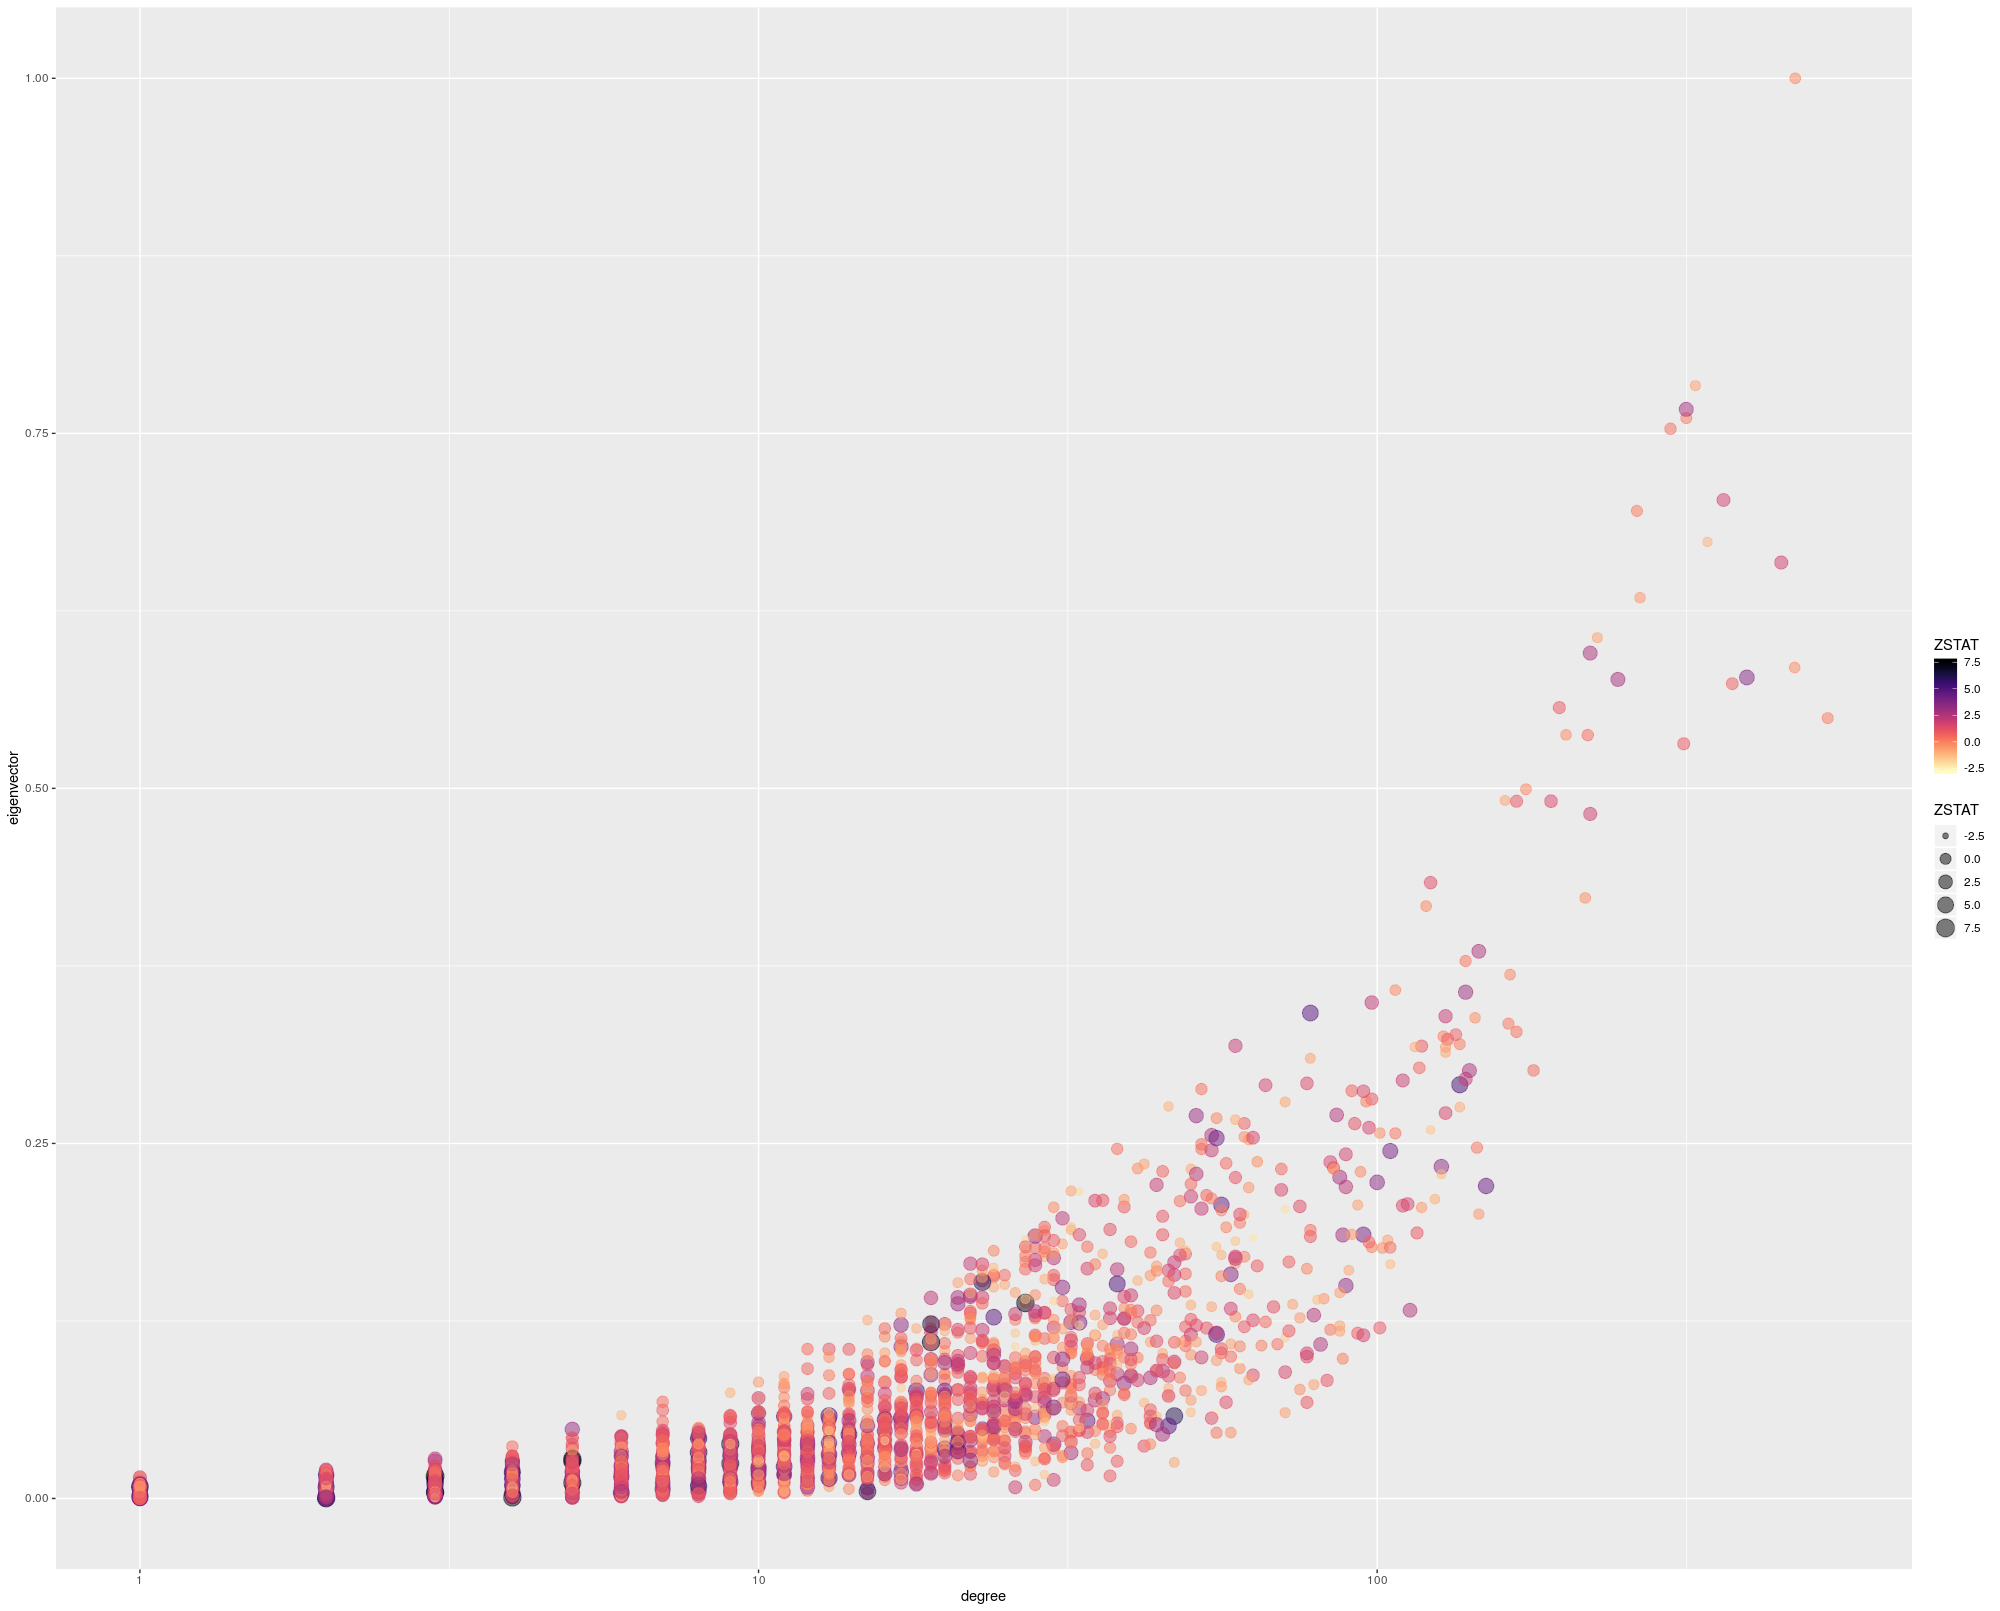
\includegraphics[width=\textwidth]{images/chapter3/ggplot2/correlation_centrality_significance/Rplot_degree_and_eigenvector_z.png}
    \caption{Plot of Intelligence\textsubscript{Discovery} eigenvector centrality and degree centrality scatterplot. Plot size and colour display Z score of significance for each gene. There is no obvious pattern of association}
    \label{fig:my_label}
\end{figure}

\section{Removed and changed figures}


\subsection{Powerlaw}

\begin{figure}
    \centering
    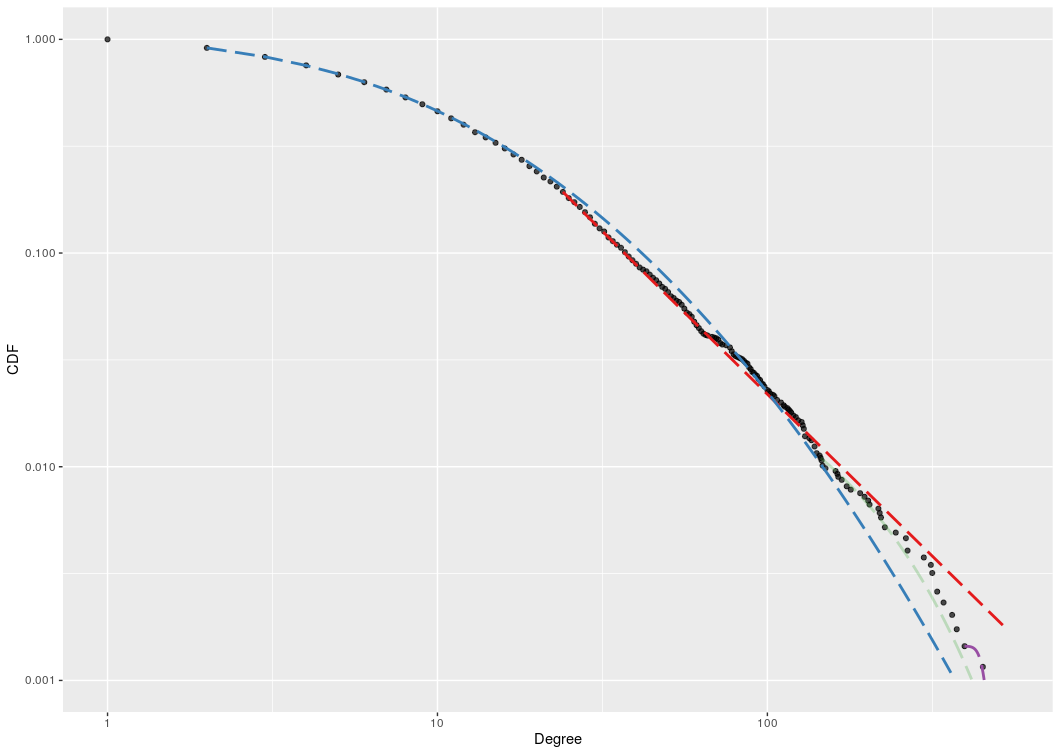
\includegraphics[width=\textwidth]{images/chapter3/poweRlaw/Rplot_best_fit_pl_lognorm_smaller.png}
    \caption{CDF of degree distribution and lines of best fit for power law (red), log-normal(blue) exponential(green) and poisson (purple). Poisson distribution is clearly a poor fit with x min close to x max (396) and the exponential distribution holds only in x min greater than 145. x axis degree log 10 scaled, y axis CDF log 10 scaled. Exponential appears a good fit but is fitted to a much smaller part of the distribution than the power law and log-normal. Poisson distribution is clearly not a good fit. \url{source('~/RProjects/chapter3/R/fit_power_law/graphing/plot_power_law_and_lognormal_ggplot2.R')}}
    \label{fig:CDF degreel}
\end{figure}

\begin{figure}
  \begin{subfigure}{7cm}
    \centering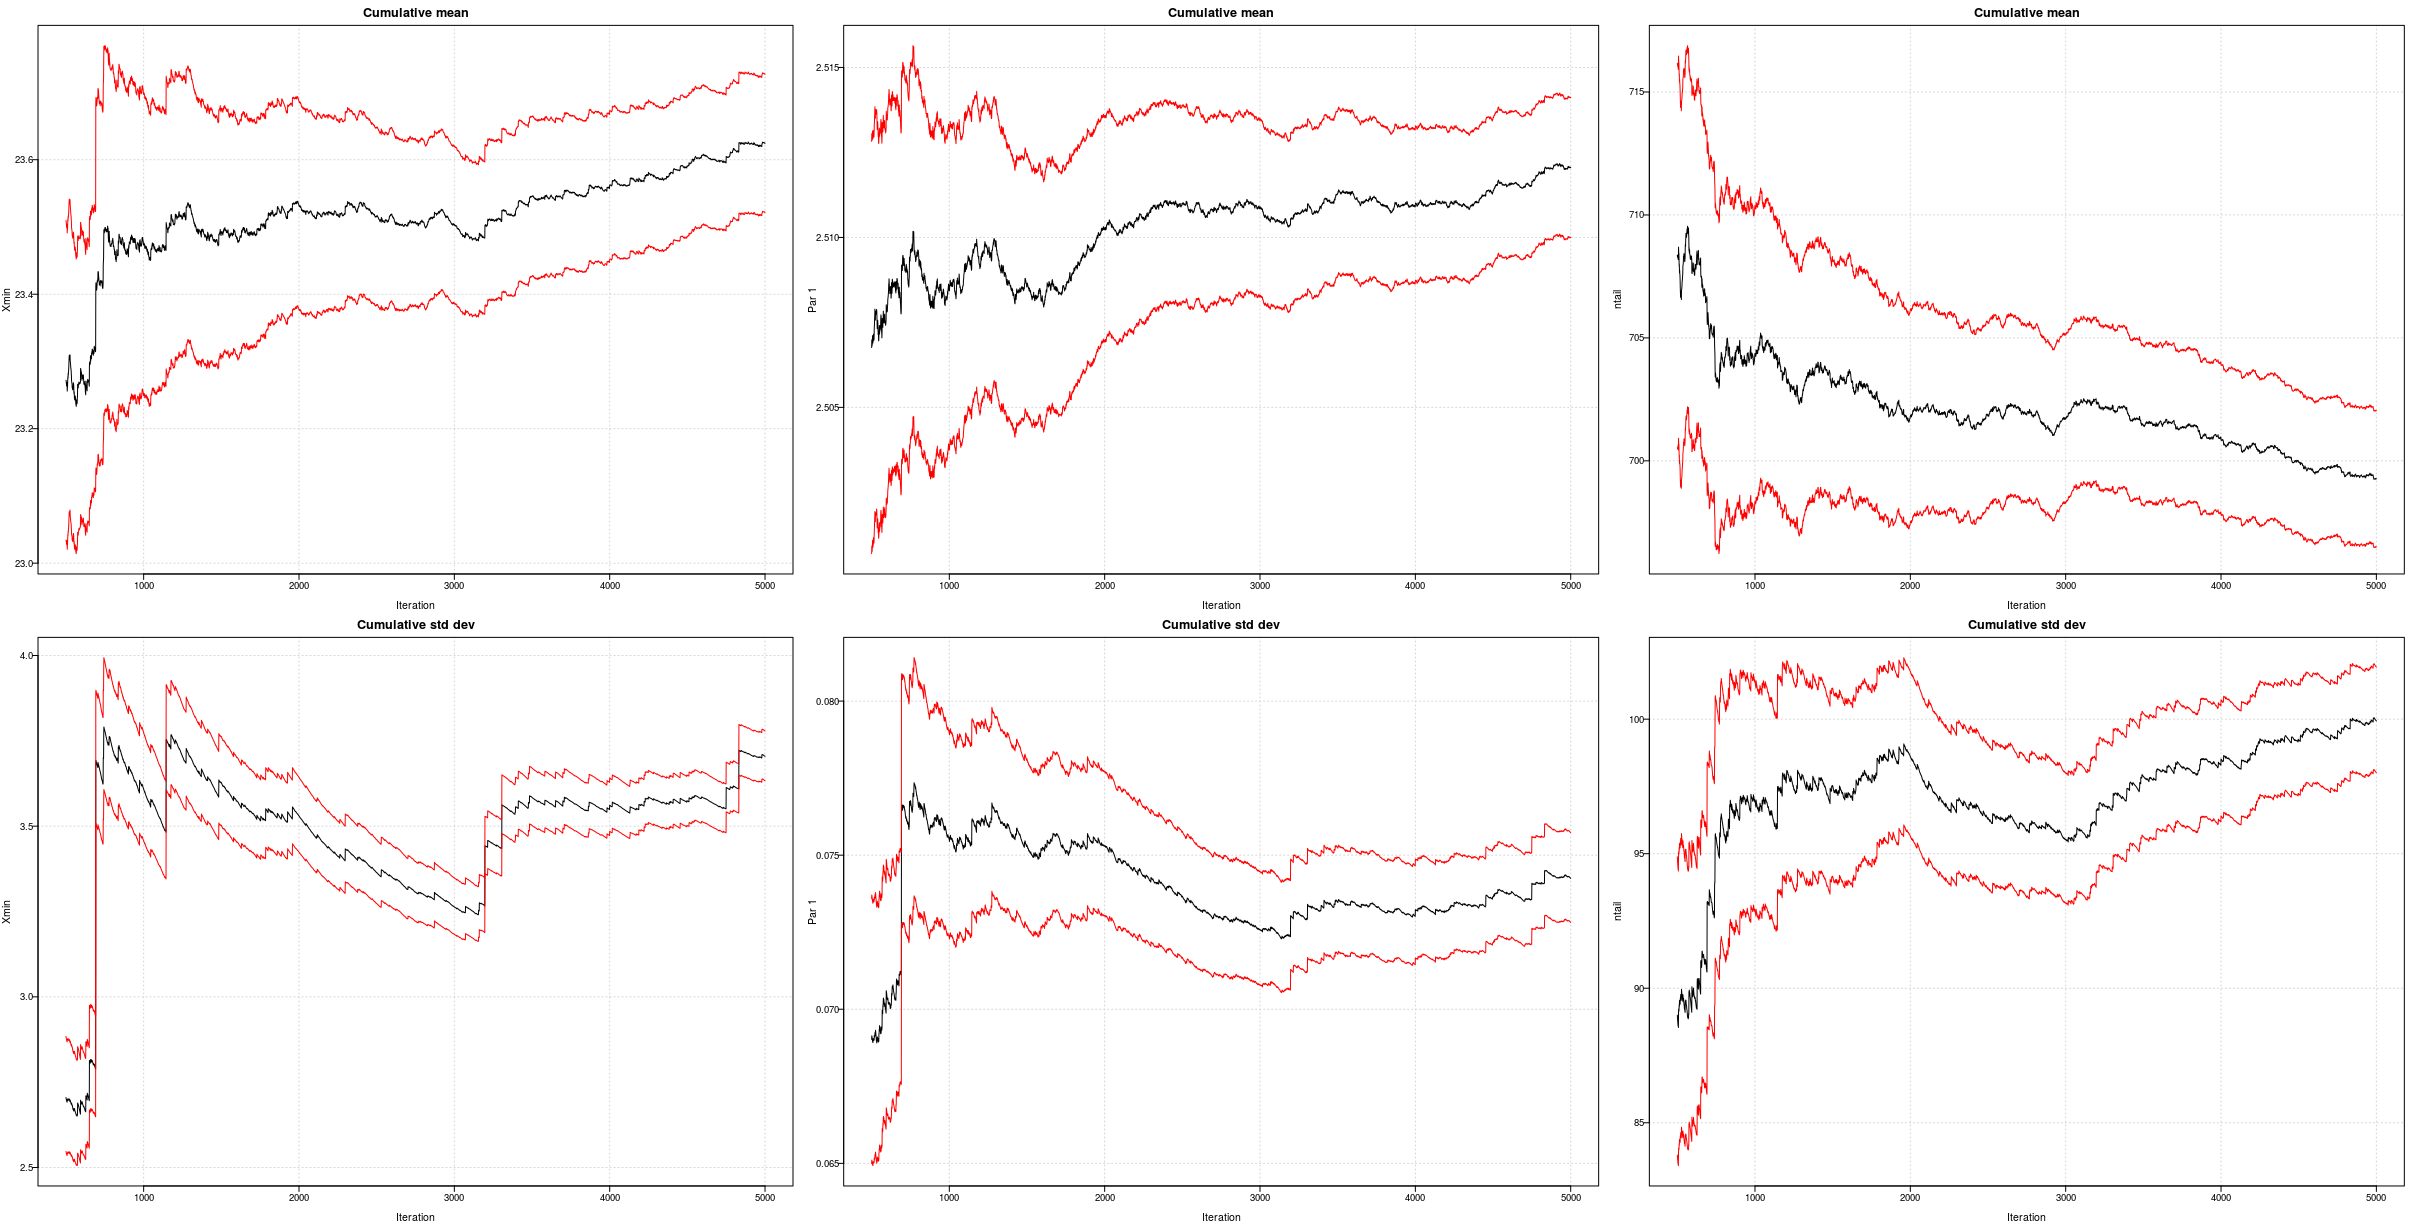
\includegraphics[width=7cm]{images/chapter3/poweRlaw/bootstrap_params/bootstrap_powerlaw_params_5000_iters.png}
    \caption{Power law}
    \end{subfigure}
  \begin{subfigure}{7cm}
    \centering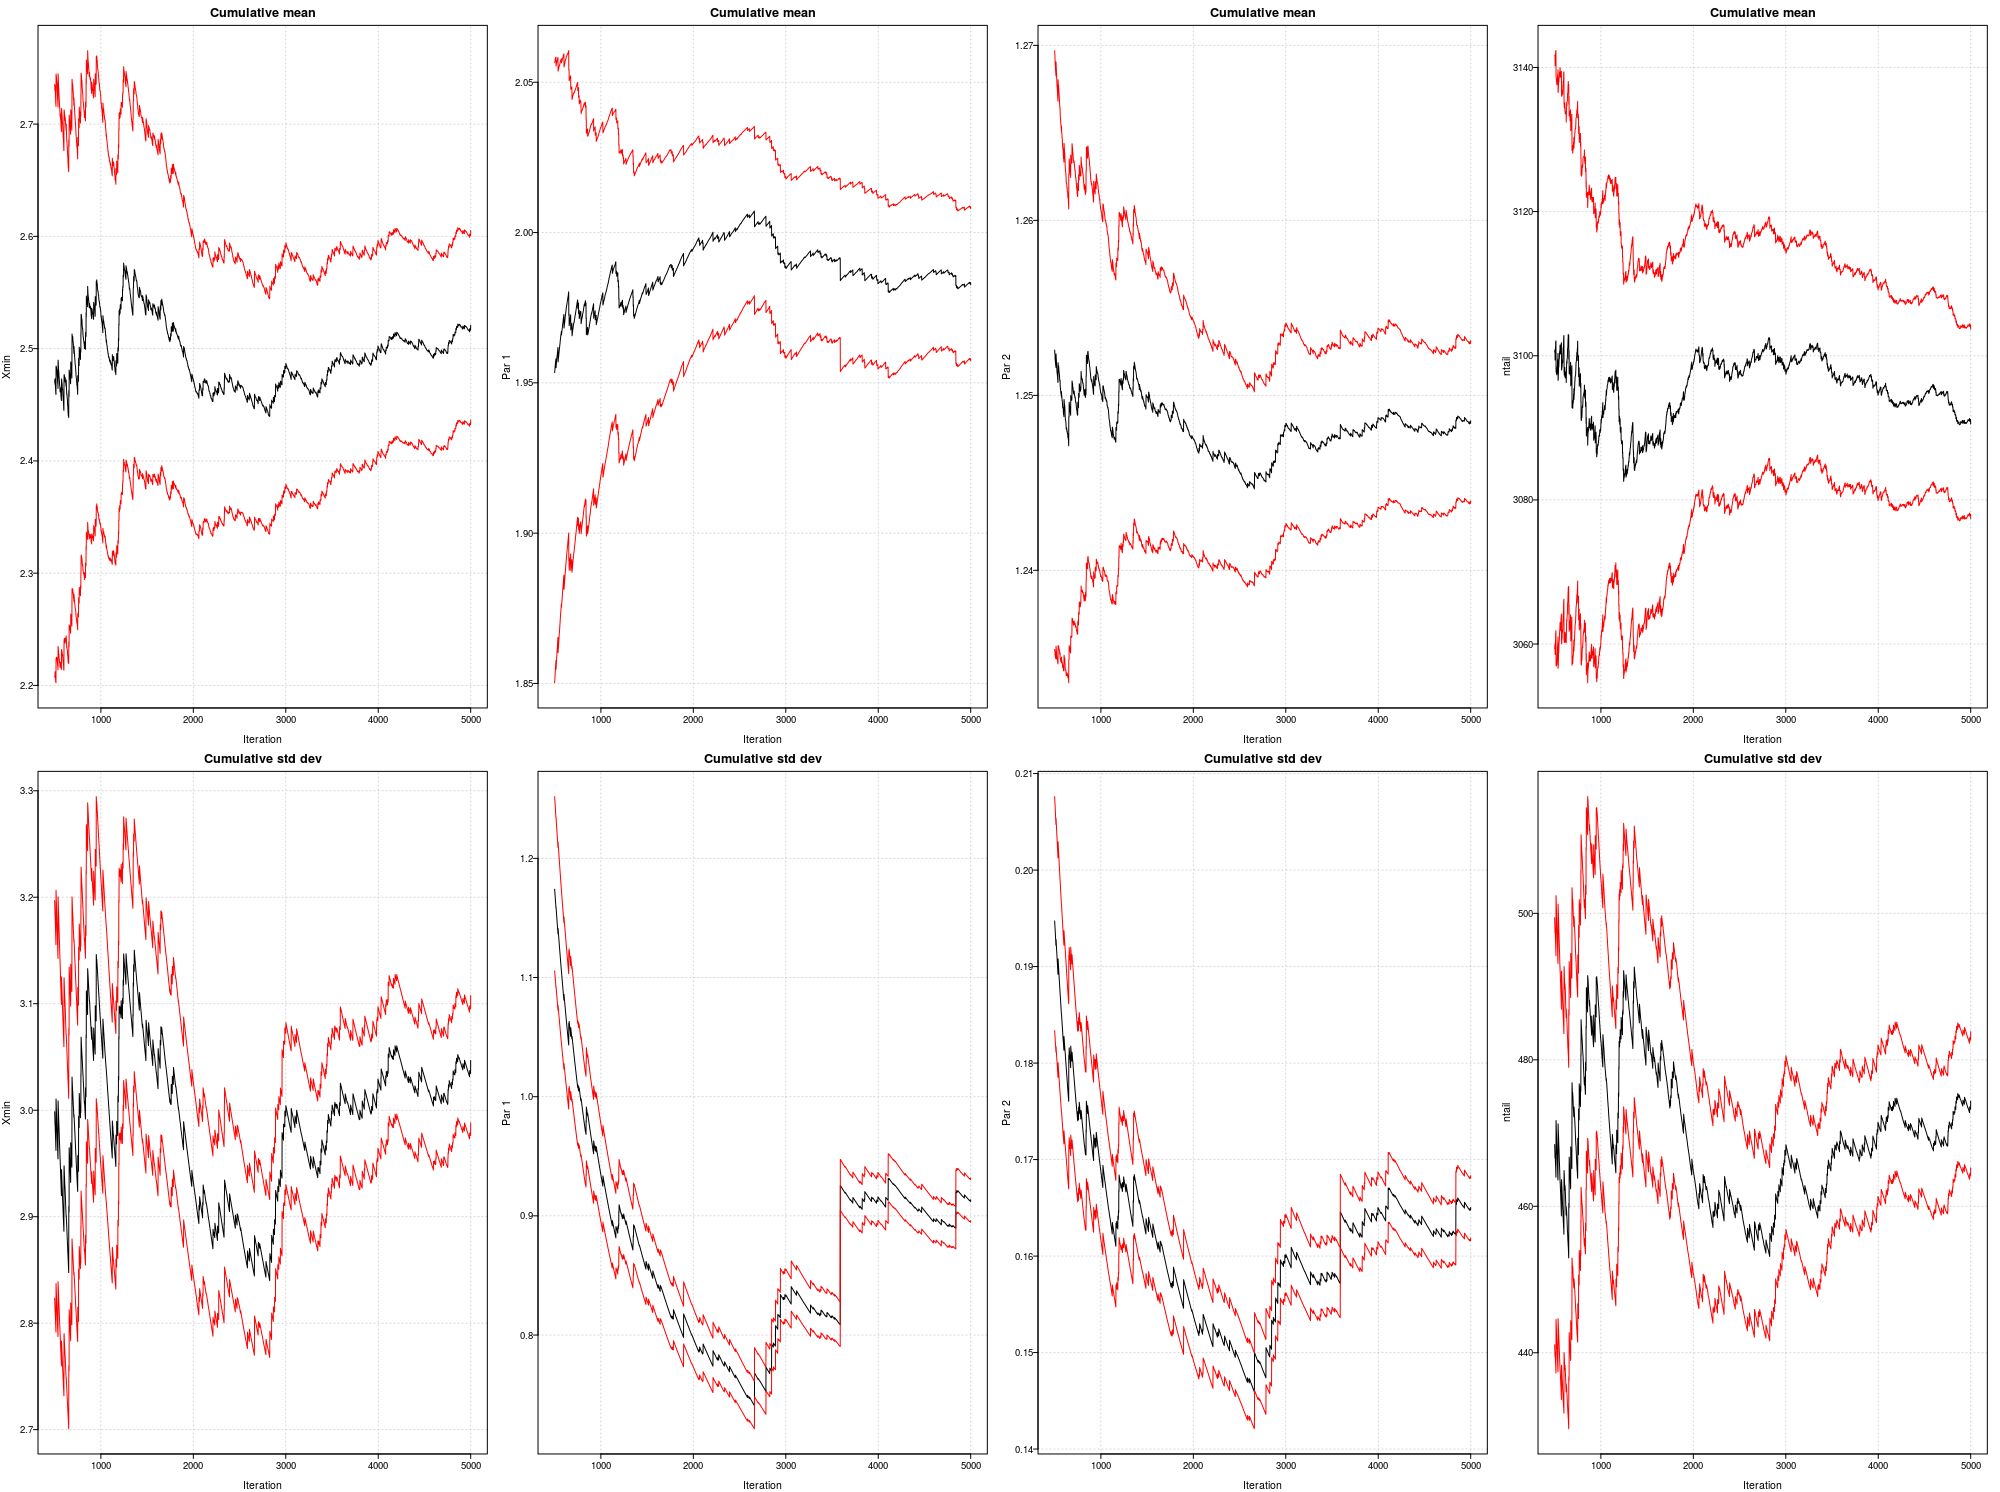
\includegraphics[width=7cm]{images/chapter3/poweRlaw/bootstrap_params/log_normal_bs_params.png}
    \caption{log-normal}
  \end{subfigure}
  \begin{subfigure}{7cm}
    \centering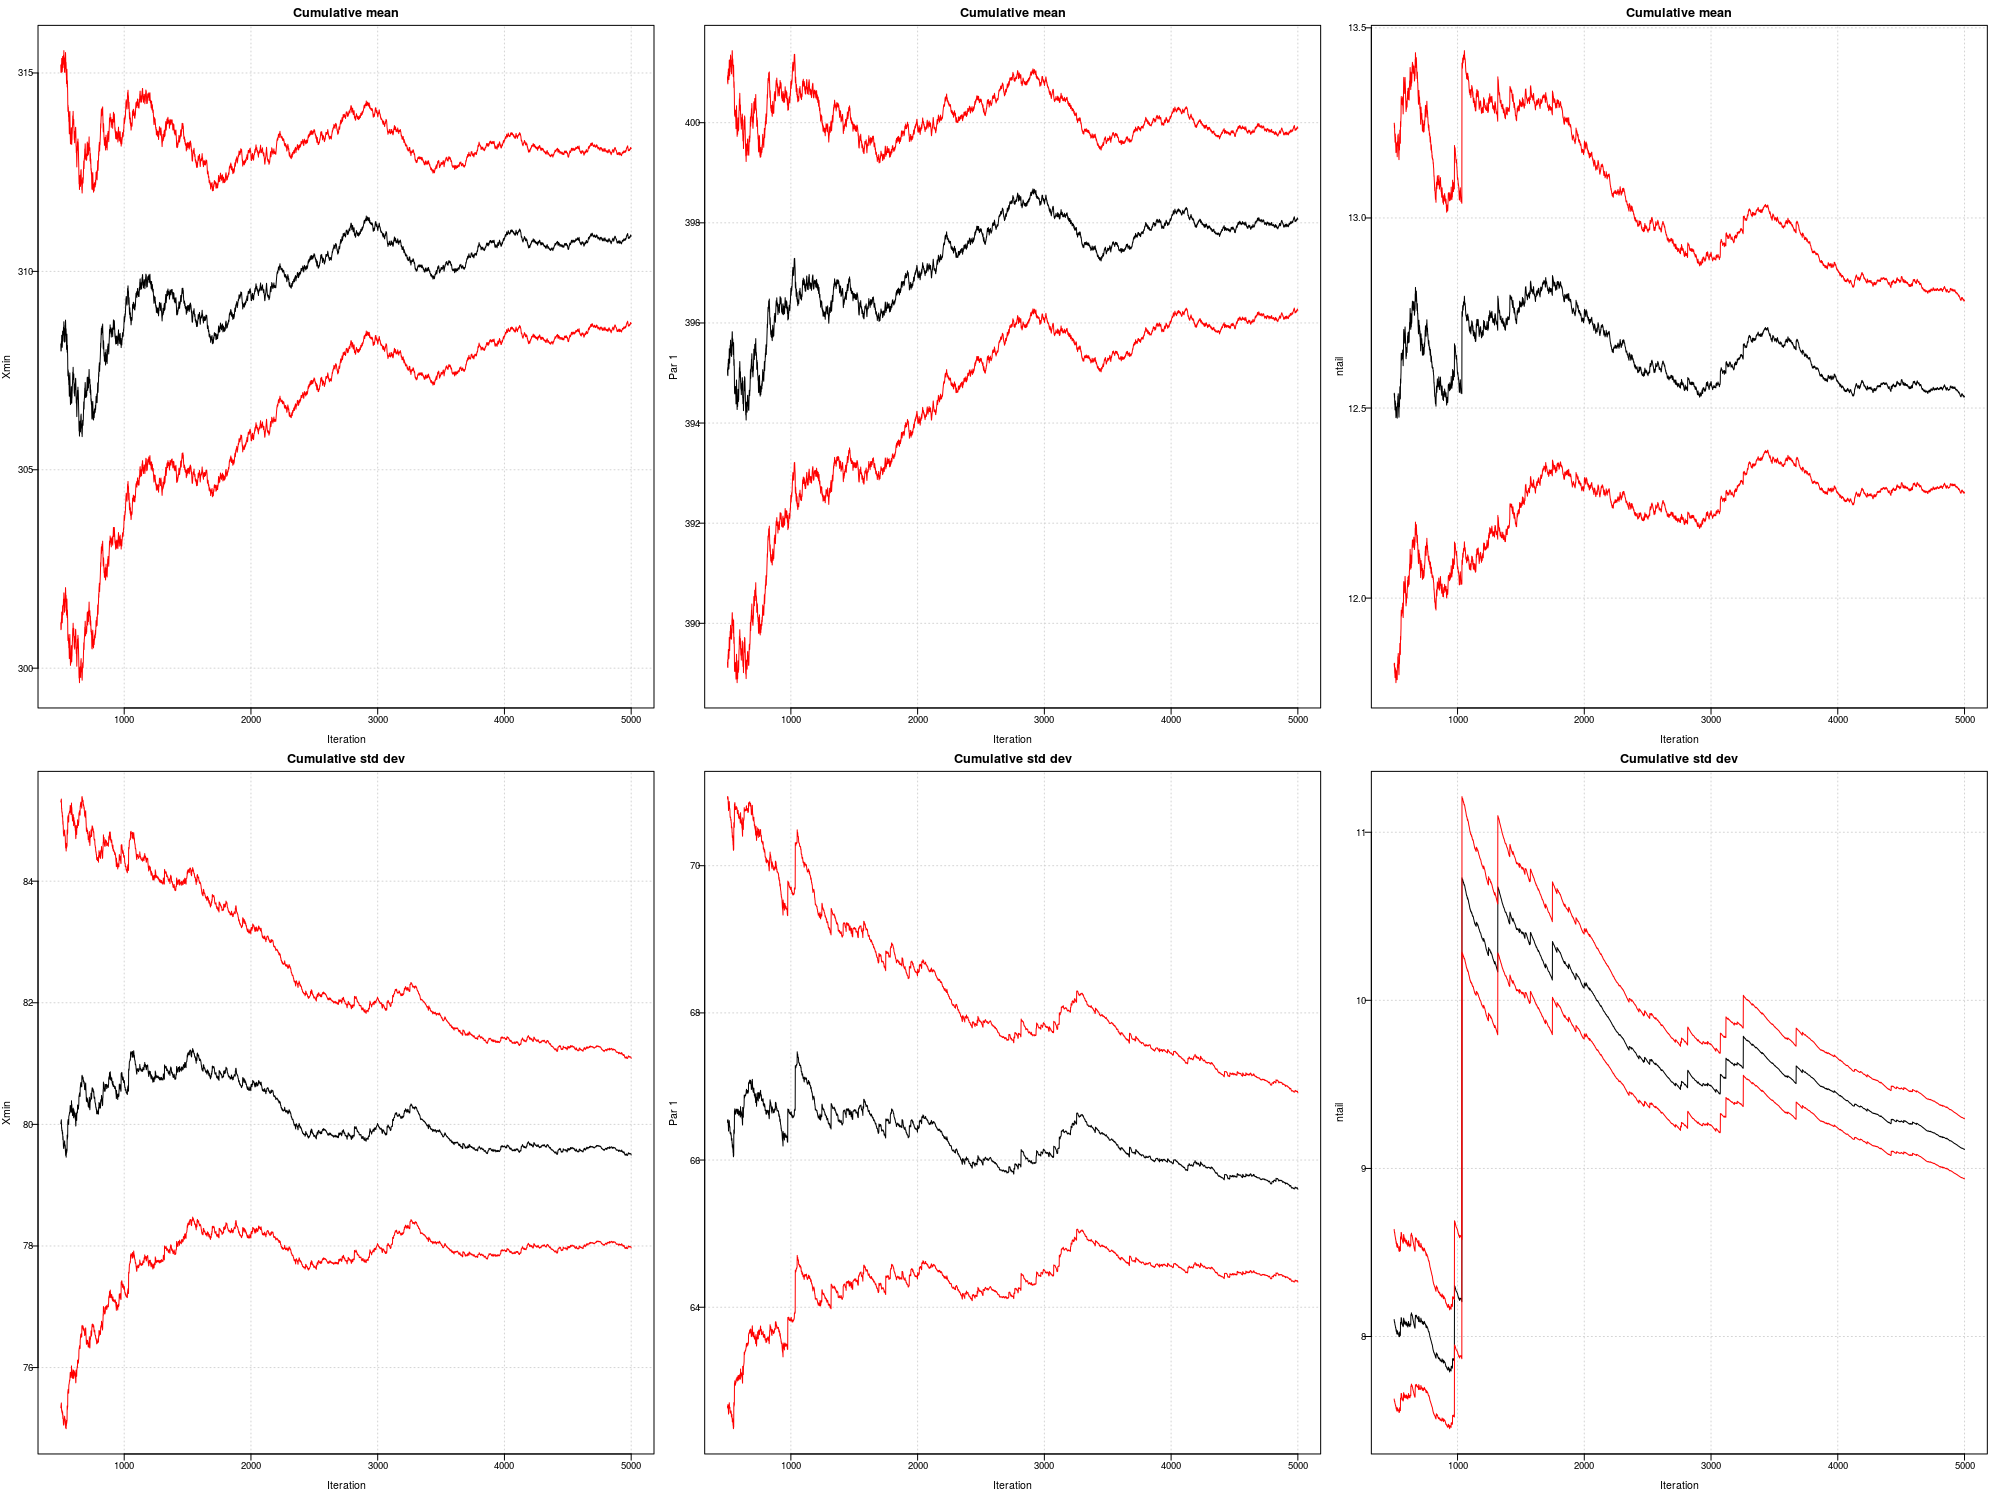
\includegraphics[width=7cm]{images/chapter3/poweRlaw/bootstrap_params/poisson_bootstrap_params.png}
    \caption{Poisson}
  \end{subfigure}
  \begin{subfigure}{7cm}
    \centering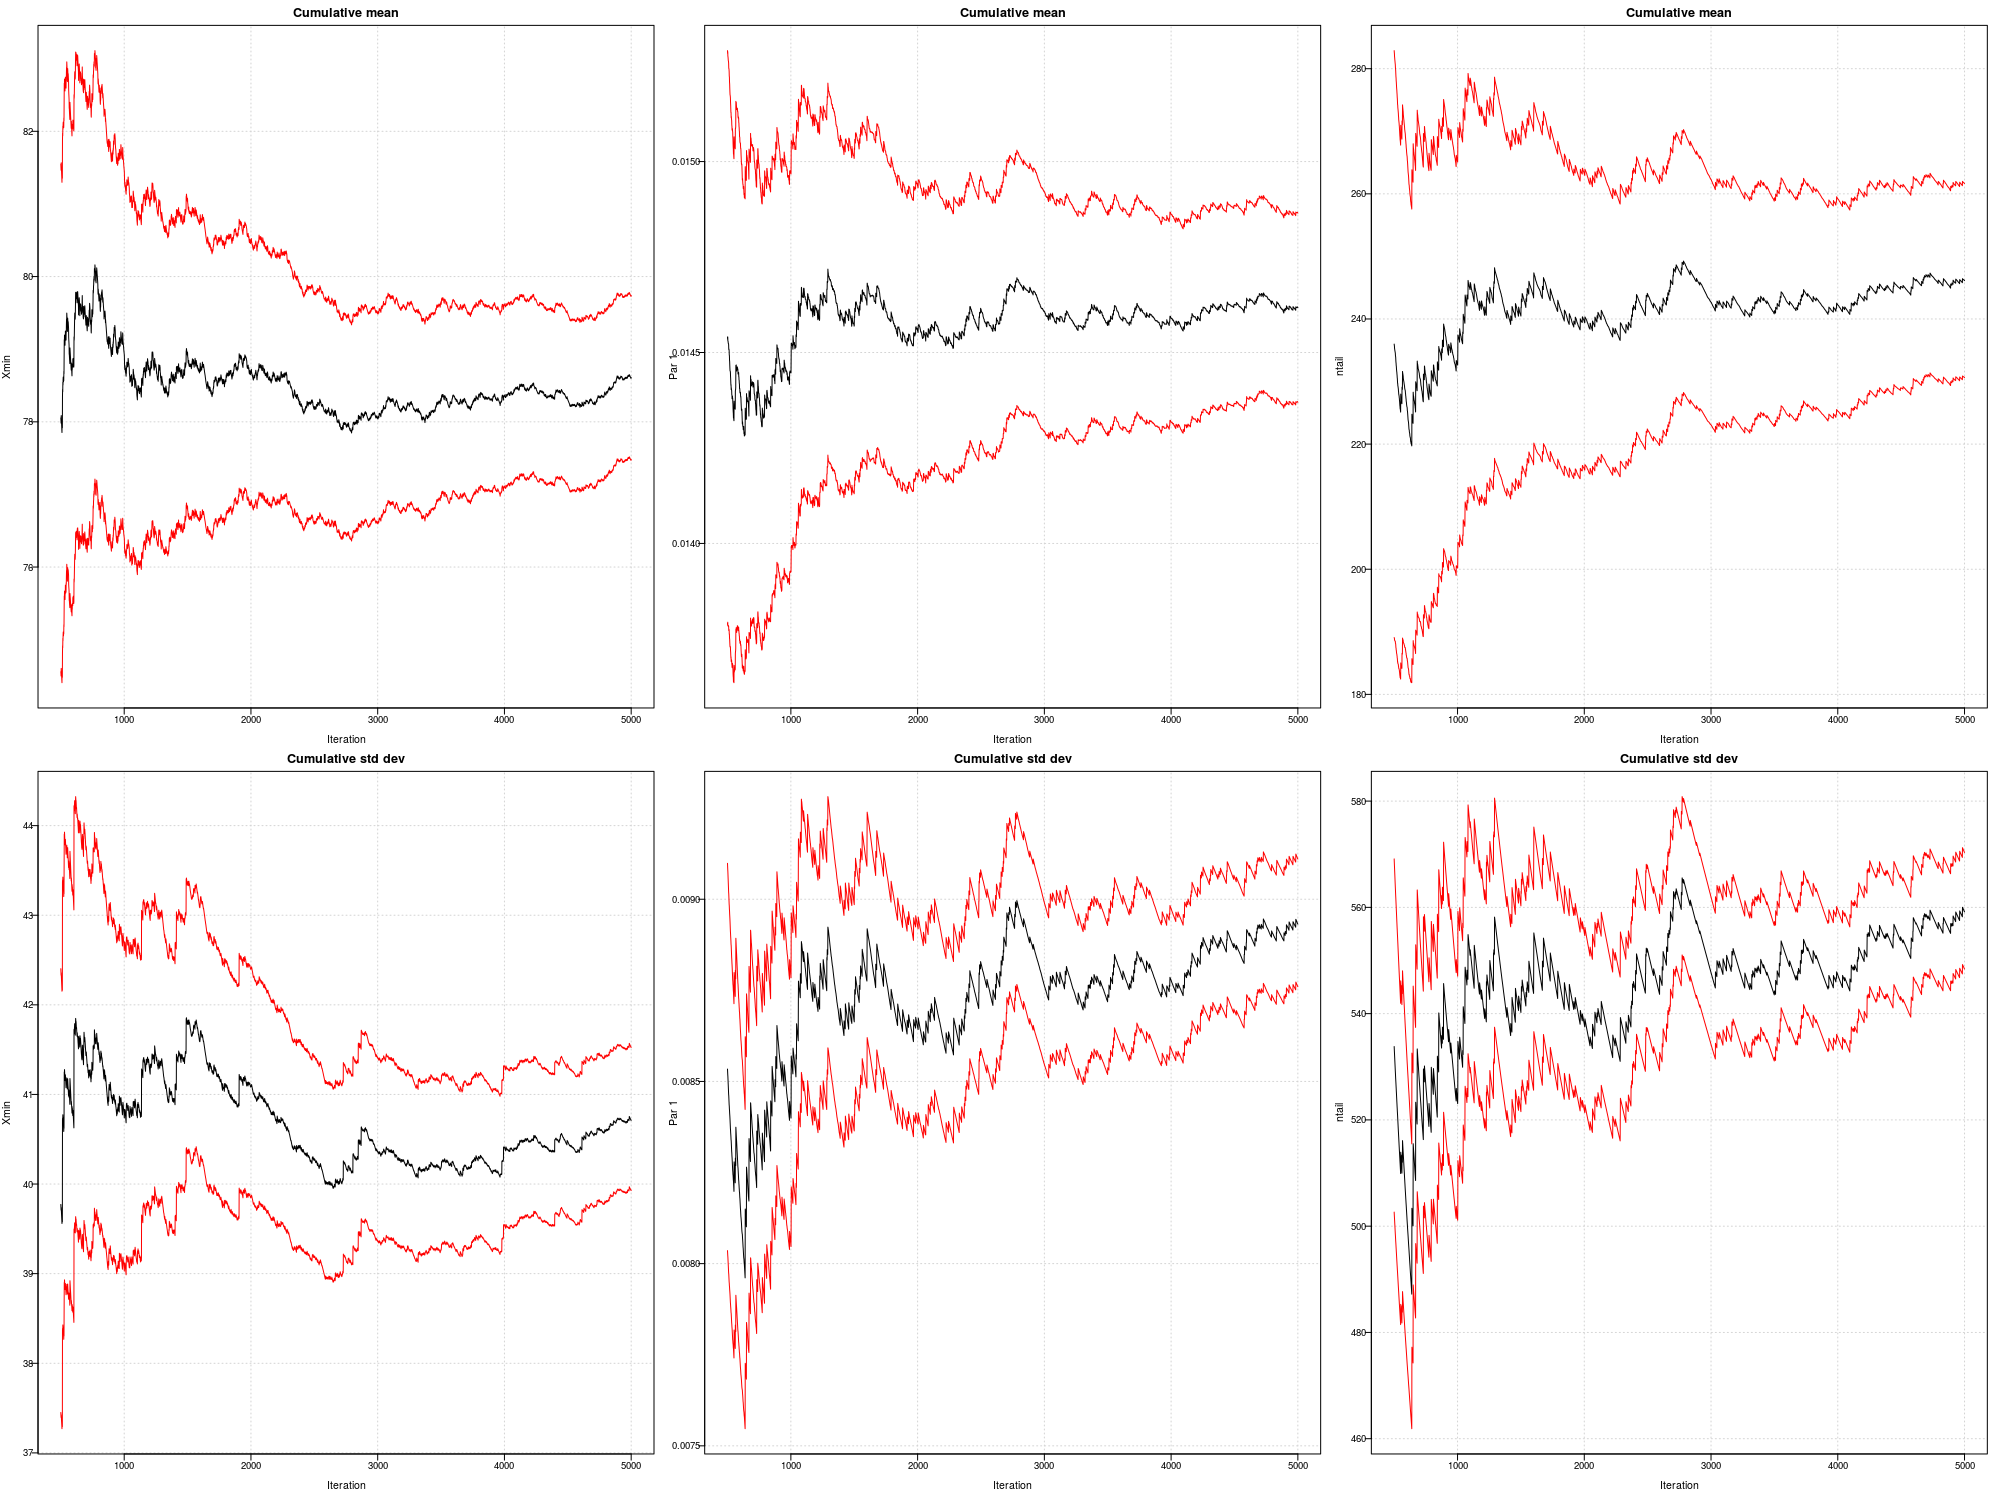
\includegraphics[width=7cm]{images/chapter3/poweRlaw/bootstrap_params/bootstrap_exp_params.png}
    \caption{Exponential}
  \end{subfigure}
  \caption[\textbf{Bootstrap estimate of degree distribution parameters}]{Bootstrap estimate of degree distribution parameters using poweRlaw package \cite{gillespie2015fitting}. }
  \label{fig:bootstrap_params}
\end{figure}


\subsection{transitivity}
\begin{figure}
    \centering
    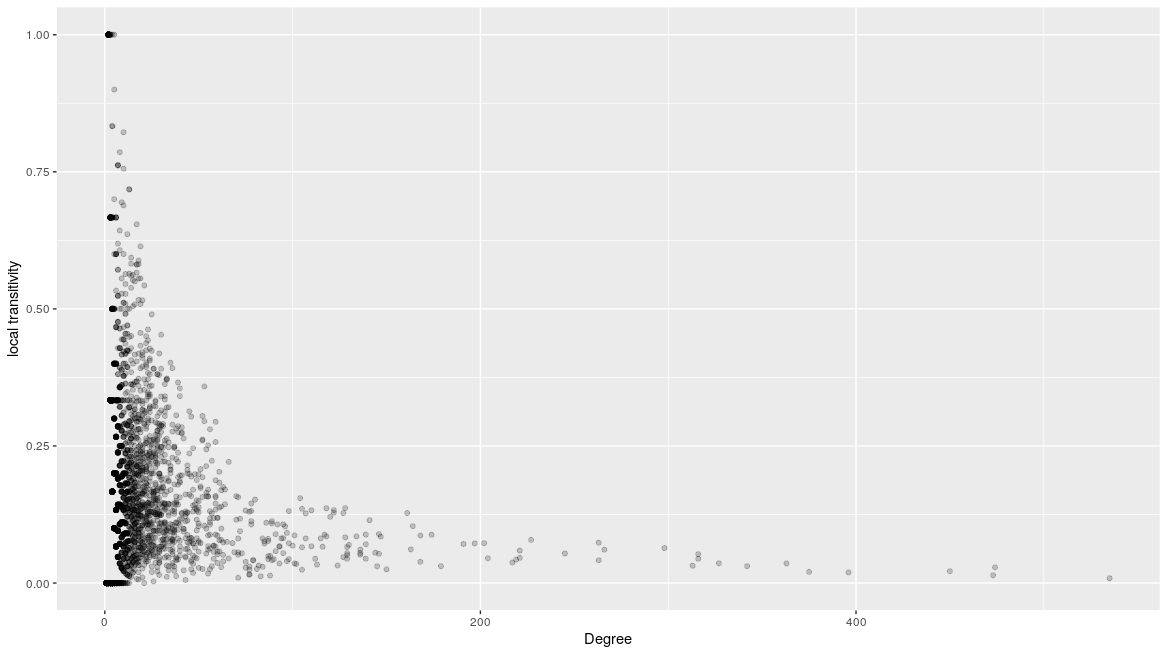
\includegraphics[width=\textwidth]{images/Rplot02_degree_and_transitivity-change_alpha.png}
    \caption{Scatter plot of the relationship between degree and local transitivity for the PSP nodes. Nodes with degree 1 have transitivity set to zero as transitivity in this case is undefined. Plot appears to show a negative correlation between degree and transitivity. The opacity of points has been decreased to reduce overplotting and show the increase in points at low degree. Potential replacement - \textcolor{red}{changed now} ('cant find original code \url{source('~/RProjects/chapter3/R/transitivity/transitivity_and_degree/mean_deg_seq.R')}}
    \label{fig:Scatter plot of the relationship between degree and local transitivity for the PSP nodes1}
\end{figure}

\subsection{DEG}
\subsubsection{boxplot}
\begin{figure}
    \centering
    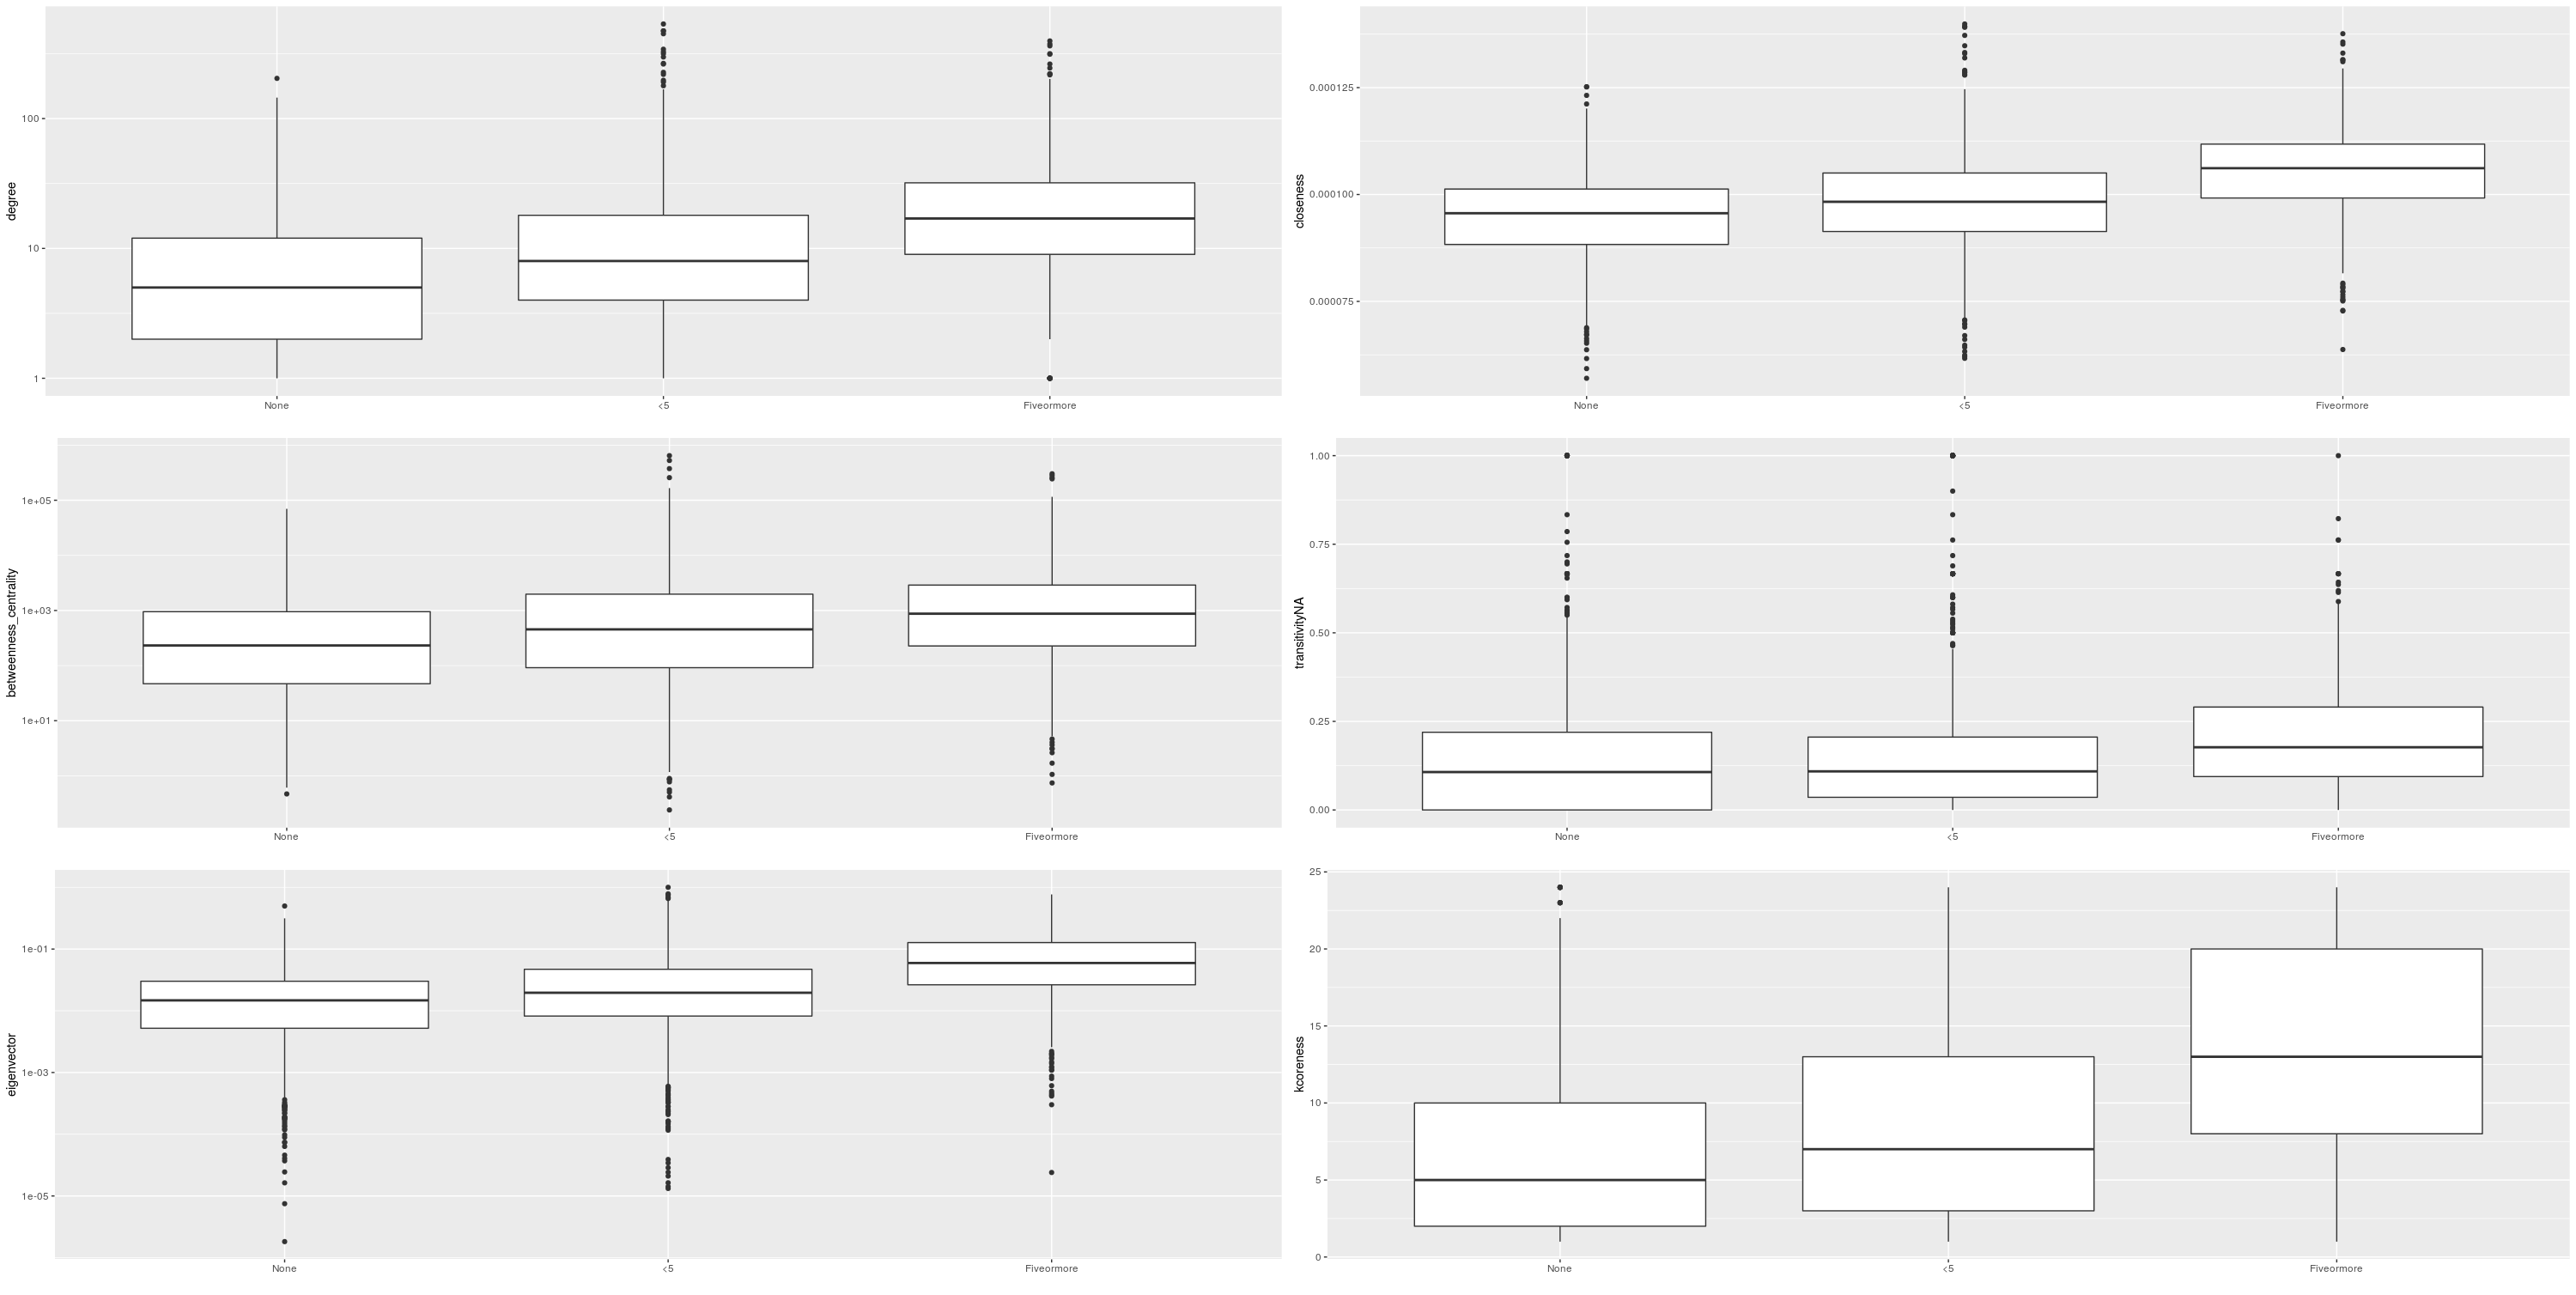
\includegraphics[width=\textwidth]{images/chapter3/ggplot2/db_essential_genes/Rplot_multiplot_centrality_deg_three_groups_no_xlab.png}
    \caption{Multiple boxplot of the centrality measure for genes in PSP and in database of essential genes(DEG). On the x axis are three groups: those genes that do not appear in the DEG, those with at least one entry but less than five and those with five or more. Y axis is log10 transform of vertex (node) degree for degree, betweenness and eigenvector centrality. The graph shows degree increasing across the three categories as genes become more essential. Script for this figure at \url{source('~/RProjects/db_essential_genes/R/get_essential_genes/db_2020/plots/get_db_essential_threecategoriesboxplot_multiplot_no_x_lab_essential_centrality.R') }}
    \label{fig:boxplot_three_groups_DEG_multiplot}
\end{figure}


\begin{figure}[p]
    \vspace*{-2cm}
    \makebox[\linewidth]{
        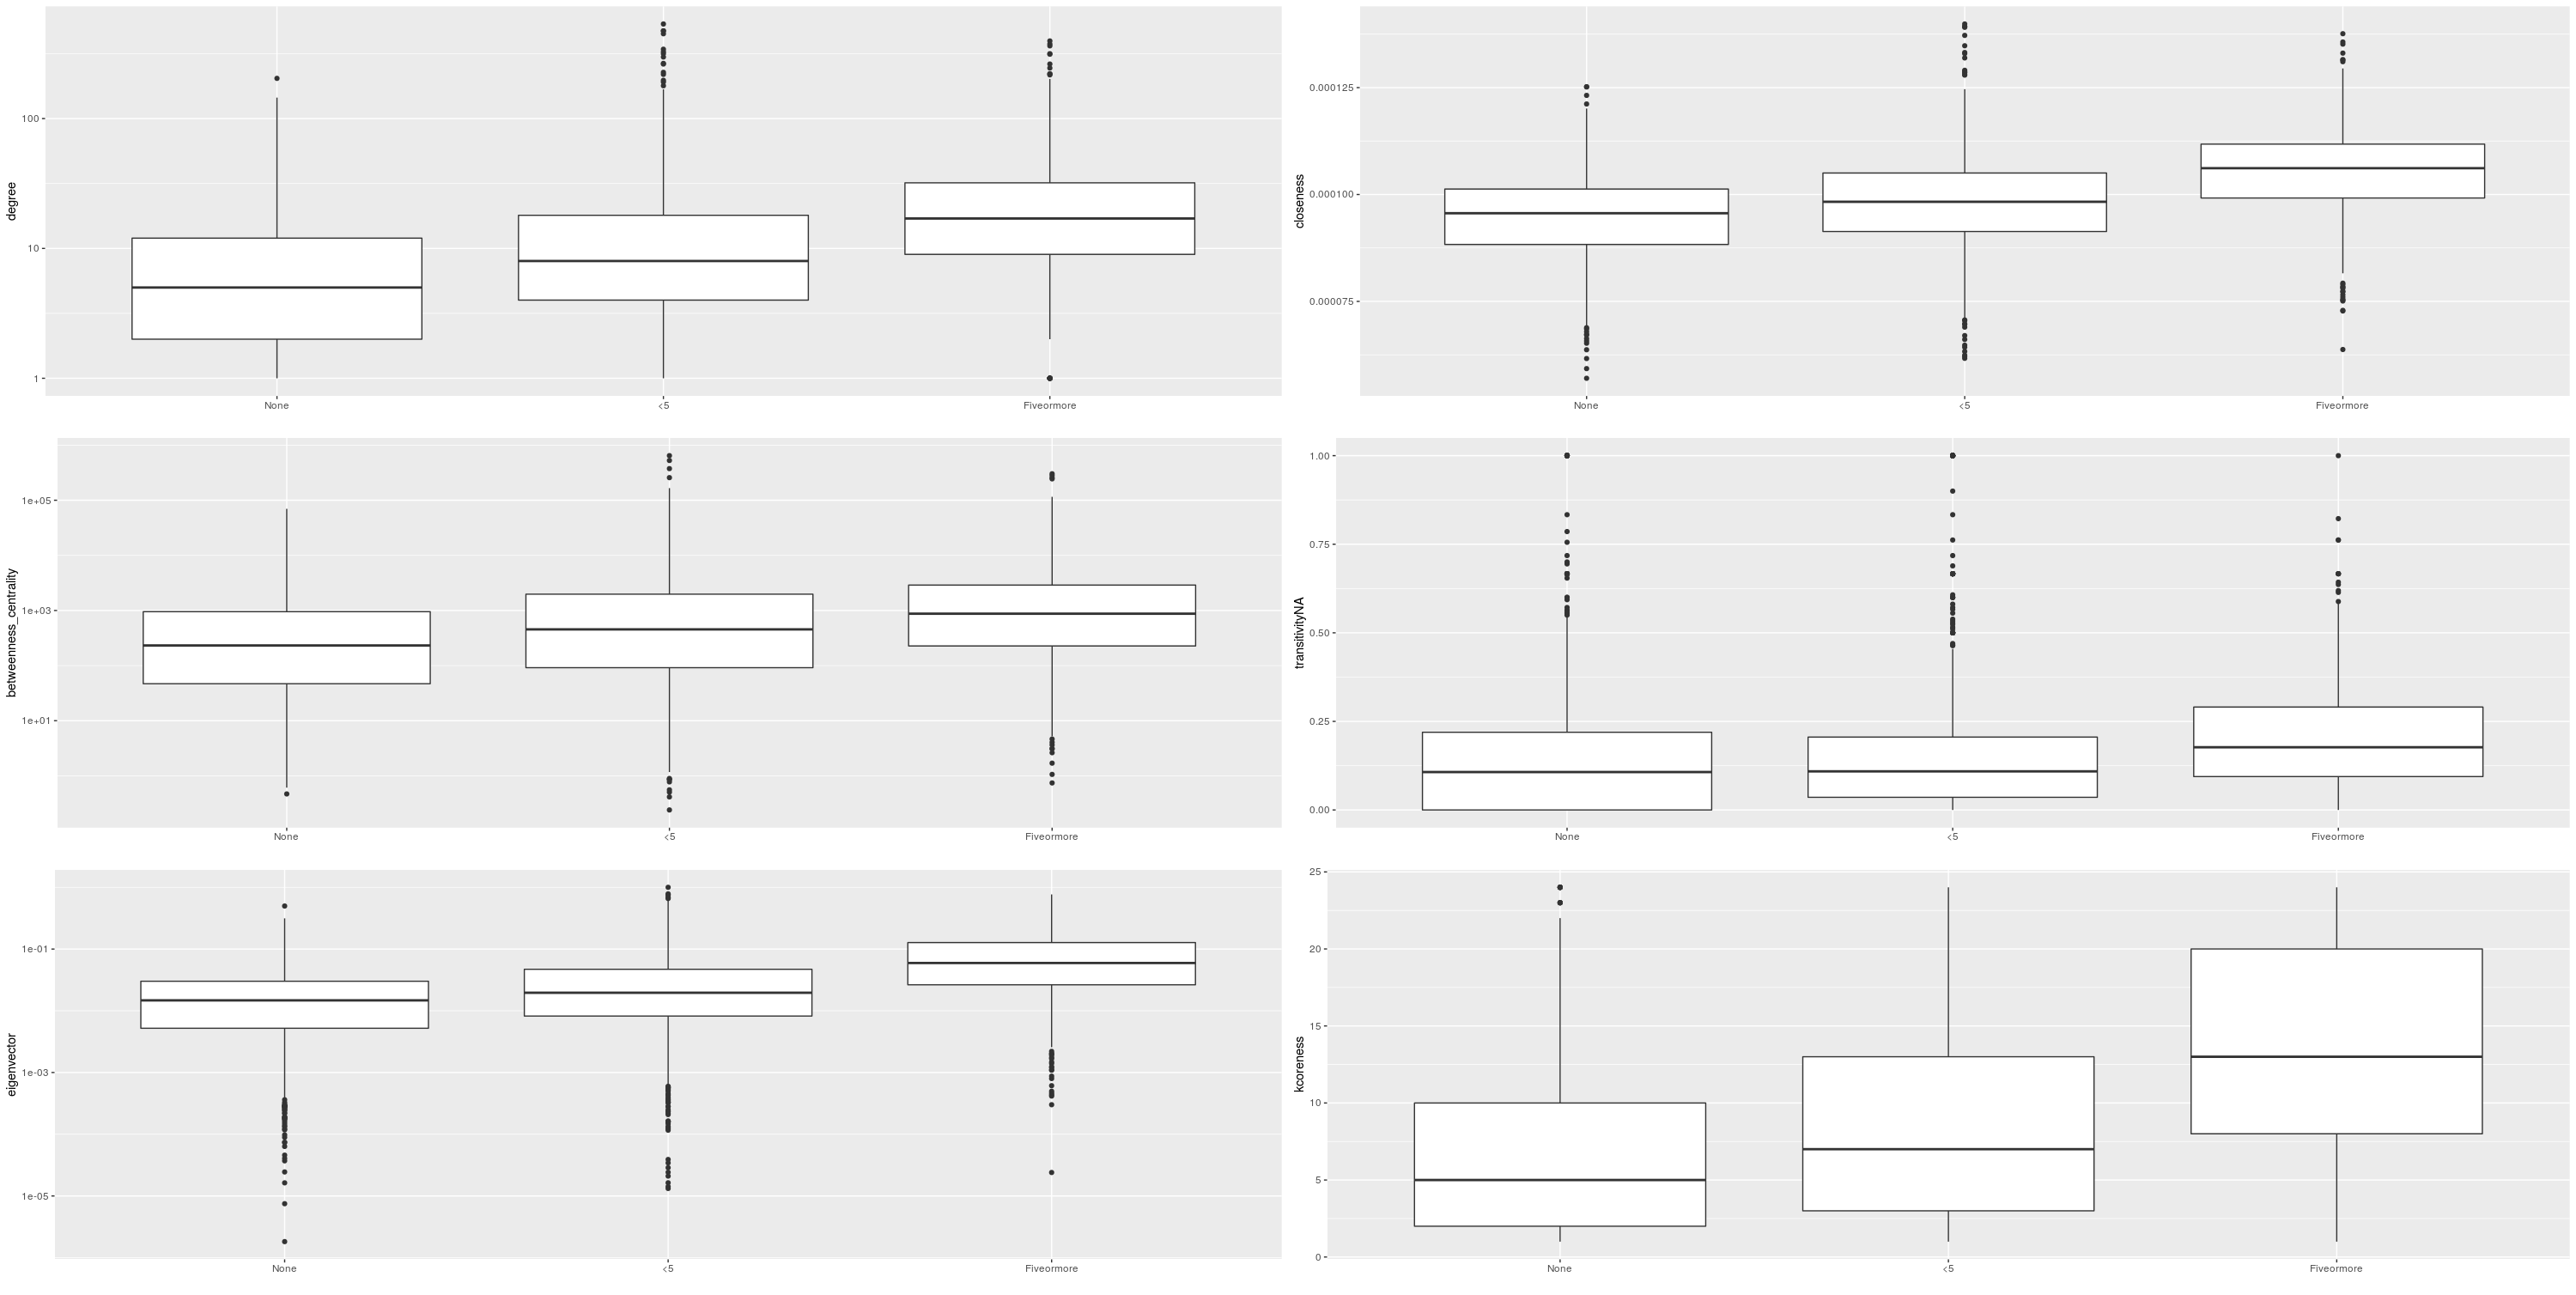
\includegraphics[width=1.3\linewidth, height=20cm]{images/chapter3/ggplot2/db_essential_genes/Rplot_multiplot_centrality_deg_three_groups_no_xlab.png}}
    \caption{Multiplot of boxplot of centralities and DEG. On the x axis categories are non essential, Up to 5 appearances in DEG, 5 or more appearances in DEG }
\end{figure}
\subsection{Gnomad}

\begin{figure}
    \centering
    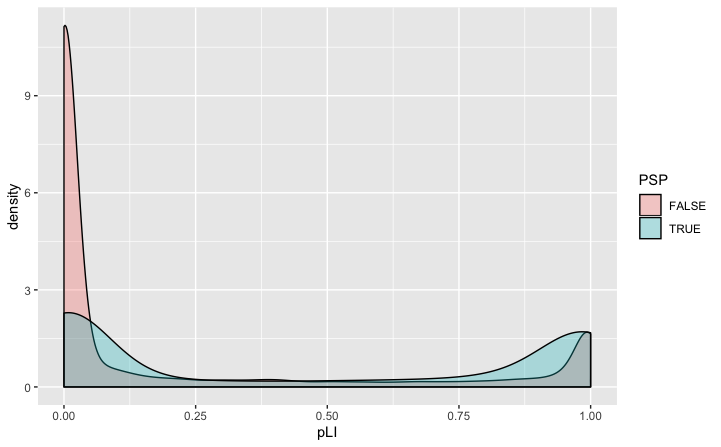
\includegraphics[width=\textwidth]{images/chapter3/ggplot2/gnomad/Rplot_density_plot.png}
    \caption{Density plot of pLI for PSP and non PSP. The distribution of probability loss intolerance is bimodal for both the PSP and non PSP genes but is more symmetrical for the PSP genes which shows a similar density of very high and very low probability of loss intolerance (pLI) values compared with the non PSP genes which, if they have extreme values are more likely to have low pLI  \url{source('~/RProjects/db_essential_genes/R/gnomad/histogram_pli_psp/density_pli_psp.R')}}
    \label{fig:densityPLI}
\end{figure}

\begin{figure}



    \centering
    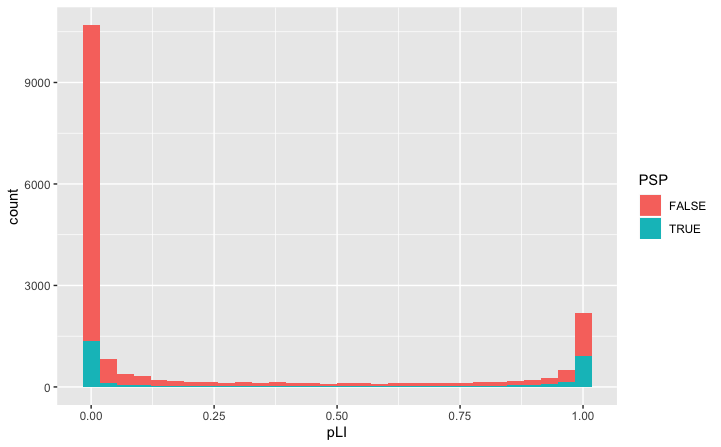
\includegraphics[width=\textwidth]{images/chapter3/ggplot2/gnomad/Rplot_PSP_gnomad.png}
    \caption{Plot of pLI for PSP and non PSP \url{source('~/RProjects/db_essential_genes/R/gnomad/histogram_pli_psp/histogram_pli_psp.R')}}
    \label{fig:hist_pliPSP}
\end{figure}
\subsubsection{Native R Density plot}

\begin{figure}
    \centering
    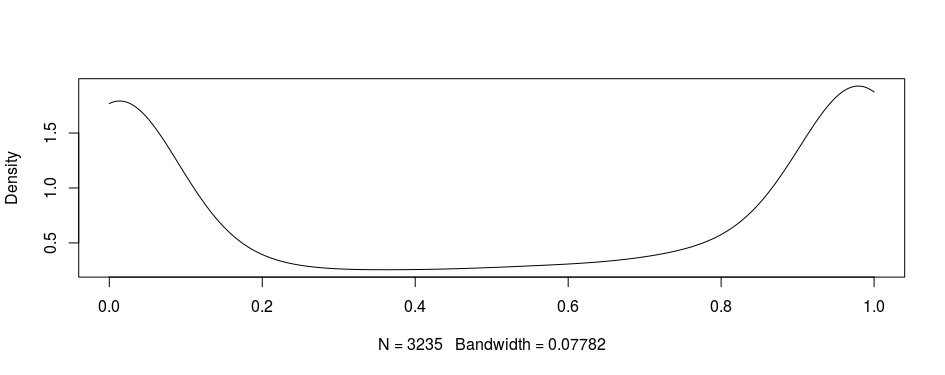
\includegraphics[width=0.9\textwidth]{images/Rplot_kernel_density.png}
    \caption{The distribution of probability of loss of function intolerance. Kernel density estimate using Guassian kernel. Bimodal distribution with peak close to 0 and 1 for the post synaptic proteome. }
    \label{fig:density estimate pLi}
\end{figure}

\begin{figure}
    \centering
    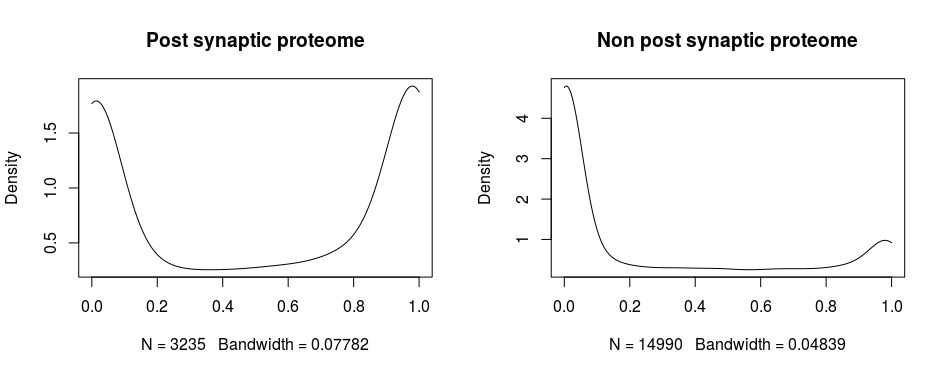
\includegraphics[width=0.9\textwidth]{images/Rplot01_density_PSP_two_panel_nonPSP.png}
    \caption{The distribution of probability of loss of function intolerance for the post synaptic proteome (left) and the rest of the genome (post synaptic proteome removed) on the right. Kernel density estimate using Guassian kernel. Bimodal distribution with peak close to 0 and 1 for the post synaptic proteome. The peak around 1 is much smaller in the non post synaptic proteome. }
    \label{fig:density estimate pLi two panel}
\end{figure}
\subsection{PCA smaller}

\begin{figure}
\centering
\begin{subfigure}{.5\textwidth}
  \centering
  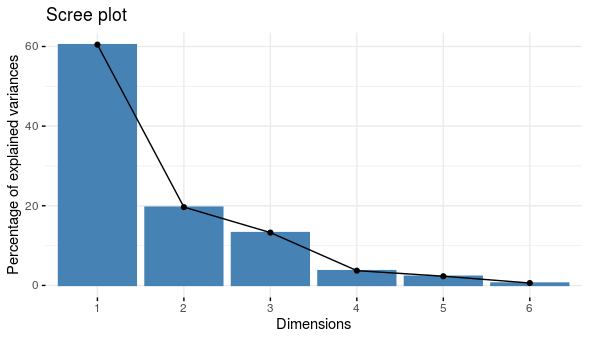
\includegraphics[width=.9\linewidth]{images/chapter3/centrality_pca_factoextra/Rplot_screeplot.png}
  \caption{Screeplot}
  \label{fig:sub1}
\end{subfigure}%
\begin{subfigure}{.5\textwidth}
  \centering
  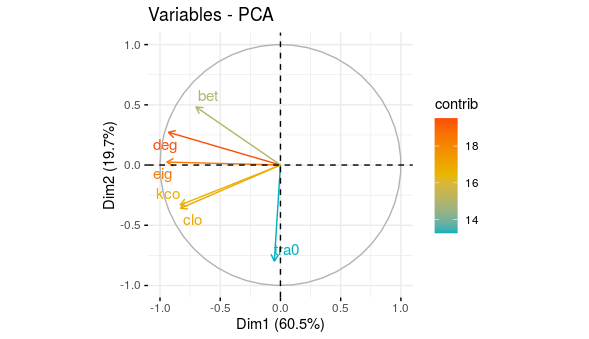
\includegraphics[width=.9\linewidth]{images/chapter3/Rplot_smaller_pca.png}
  \caption{Contribution of variables}
  \label{fig:sub2}
\end{subfigure}
\caption{Principal component analysis of centrality measures{Screeplot of the dimensions of centrality. TransitivityNA has been omitted to avoid dealing with NA. \url{source('~/RProjects/chapter3/R/centrality_ch3/prcomps/3_plotPCA.R')}}Contribution of different variables. deg = degree, eig = eigenvector centrality, kco = kcore index, tra0 = transitivity with isolates set to zero, clo = closeness, bet = betweenness centrality.  \url{source('~/RProjects/chapter3/R/centrality_ch3/prcomps/3_plotPCA.R')}\url{https://tex.stackexchange.com/questions/37581/latex-figures-side-by-side}}
\label{fig:test}
\end{figure}

\subsection{Murine LTP and centrality}
\begin{figure}
    \centering
    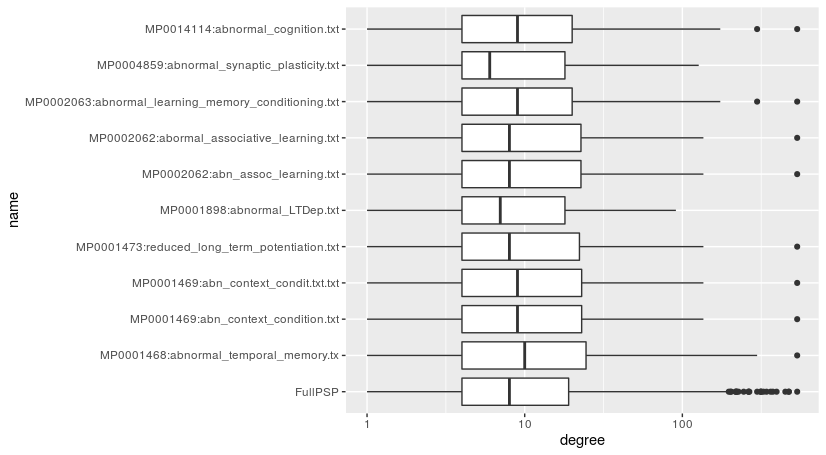
\includegraphics[width=\textwidth]{images/chapter3/ggplot2/murine_centrality_boxplot/Rplot_degree_centrality_rough.png}
    \caption{Box plot of Degree centrality distribution for differenet gene sets affecting Murine LTP or learning. Log 10 scale for degree. No statistically significant difference other than minor change in long term depression. \url{source('~/RProjects/chapter3/R/murine_centrality/rough_centrality_boxplot_murine_ltp_degree.R')}}
    \label{fig:murine_ltp_centrality_boxplot_degree}
\end{figure}

\begin{figure}
    \centering
    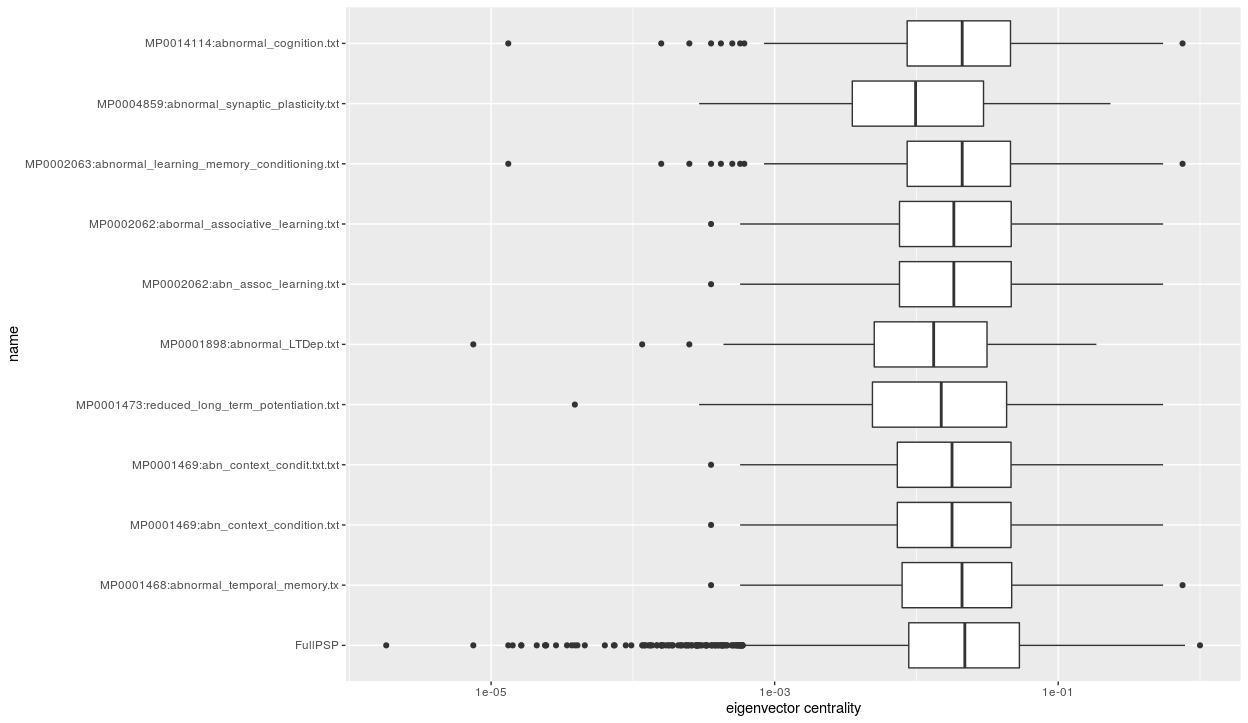
\includegraphics[width=\textwidth]{images/chapter3/ggplot2/murine_centrality_boxplot/Rplot_eigenvector_rough_corrected.png}
    \caption{Box plot of eigenvector centrality centrality distribution for different gene sets affecting Murine LTP or learning. Log 10 scale for degree. No statistically significant difference other than minor change in long term depression.\textcolor{red}{recheck abnormal spatial learning not in plot. Corrected now} \url{source('~/RProjects/chapter3/R/murine_centrality/rough_centrality_boxplot_murine_ltp_eigenvector.R')}}
    \label{fig:murine_ltp_centrality_boxplot_eigenvector}
\end{figure}

\begin{figure}
    \centering
    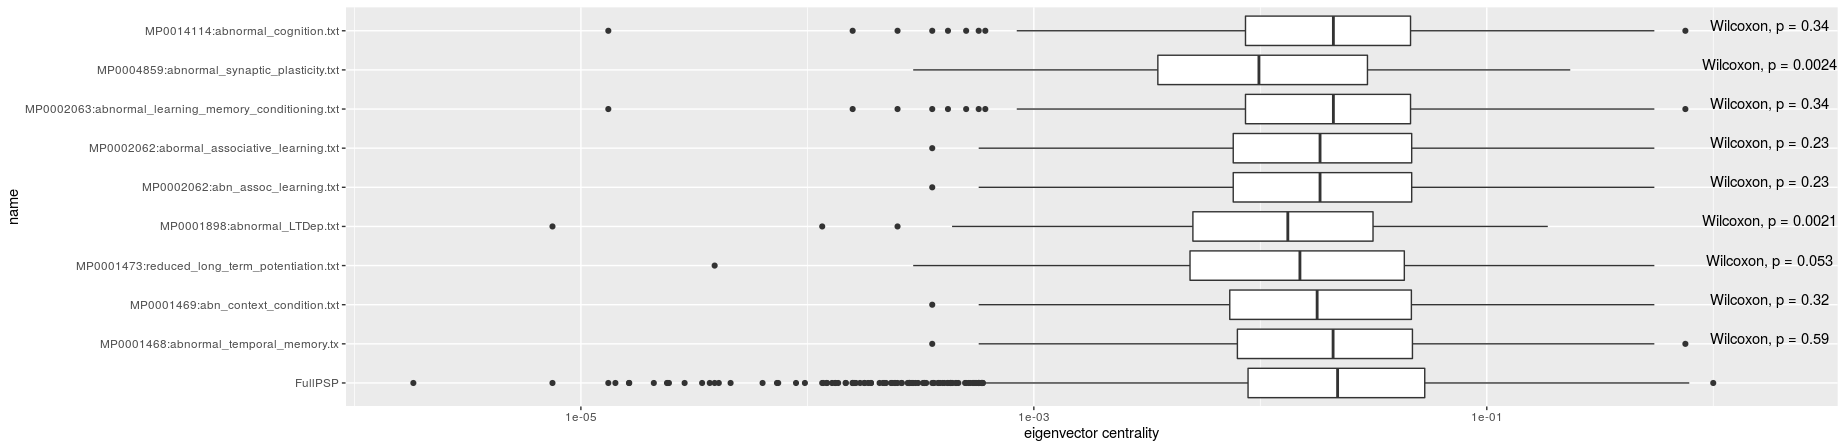
\includegraphics[width=\textwidth]{images/chapter3/ggplot2/murine_centrality_boxplot/with_p/Rplot_eigenvector_centrality.png}
    \caption{Box plot of eigenvector centrality centrality distribution for differenet gene sets affecting Murine LTP or learning. Log 10 scale for degree. No statistically significant difference other than minor change in long term depression.\textcolor{red}{recheck abnormal spatial learning not in plot. Corrected now} \url{source('~/RProjects/chapter3/R/murine_centrality/rough_centrality_boxplot_murine_ltp_eigenvector.R')}}
    \label{fig:murine_ltp_centrality_boxplot_eigenvector}
\end{figure}



\subsection{Results of correlation analysis FROM PAPER}
\textcolor{red}{Moved from earlier}
The vertex measures are correlated with one another apart from transitivity and range from 0.89 (eigenvector centrality and degree) to 0.33 (betweenness centrality and closeness centrality) (\textcolor{red}{see supplementary table 6} \todo{table}).
There is a weak negative ($\rho \approx 0.2$) correlation between 
the degree of selection pressure a gene is under and all measures of vertex importance except for transitivity (\textcolor{red}{see table 7 supplemental material} \todo{table}).
Although nodes of high importance or local clustering do have distinct properties, for example nodes with degree $> 50$ are enriched in association for the biological process (GO:1903350)‚ ”intracellular response to dopamine‚” (FDR P= 2.10 $\times 10^{-4}$ fold change 22.37), we find no correlation with these measures and genetic association with educational attainment or intelligence. 
\textcolor{green}{DRAFT -something like This is not because nodes of high degree or other centrality measure do not share common attributes, for example nodes with degree $>50$ are disproportionately found in BP intracellular dopamine but we find no association between these measures and educational attainment or intelligence}

\subsubsection{Results GO enrichment local clustering coefficient}

There was little enrichment for local clustering coefficient using GO and 0.05 and 0.95 centile in part because of the large number of 0 values when isolates are treated as 0. However in table~\ref{tab:Number of nodes 935 local transitivity 0.05 centile  local transitivity $<=$ 0 CC background PSP.Alpha=3.33555703802535e-05isolates 0} we can see that low local transitivity i.e. transitivity equal to 0 nodes (isolates) are enriched for plasma membrane components, the plasma membrane components do not show marked transitivity which is perhaps to be expected as they are at the edge of the PSP and it would not be intuitive for these components to all be interconnected. 

\subsubsection{K core gene ontology}
 
 Gene ontology enrichment for molecular  a range over the outer core 1-7 is shown in table~\ref{tab:kcore range GO Number of nodes 1724 k core 0 centile  k core1-7 MF background PSP. Alpha=3.33555703802535e-05}. It shows enrichment for trans-membrane transporters and G protein coupled receptors. 
 
 The innermost core $k>=23$ shows enrichment for RNA processing as seen in other centrality measures (table~\ref{tab:Number of nodes 201 k core 0.95 centile  k core $>=$ 23 BP background PSP. Alpha = 4.5583006655119e-06})

Code for GO and centrality measures \url{source('~/RProjects/group_sizes/R/plotting/modified_example...'} 
 
 Bassett \cite{bassett2017small} brain small world networks revisited
\subsection{Average path length}
 \label{sec:Centrality intro average path length}

\subsubsection{Commented out are bnelow on degree, giant component and comparison of degree to random}
% \subsection{Comparison of degree distribution to random erdos graph}
% \textcolor{red}{?move to introduction}
% See section~\ref{sec: intro_random_graphs}
% \todo{Comparison of degree to random graph with same p}

% \begin{equation}
%     <m> = \binom{n}{2}p
% \end{equation}


% \begin{equation}
%     c = (n-1)p
% \end{equation}
% where c is the mean degree see newman p 346

% Add a histogram here and the expected mean and quartiles.


% \subsection{Degree and giant component}
% \label{sec:connected component and degree}
% \textcolor{red}{ ?move to introduction or second chapter}
% Some structure can develop even in random graphs see~\ref{sec: intro_random_graphs}
% \todo{Change this as below subcritical, supercritical, fully connected} CHANGE this
% In a random graph there is a point at which scattered connected nodes combined to form a giant component. Subcritical to supercritical at $<k> >1$


% Supercritical to fully connected at $E[k] > \ln(N)$


% Where $N$ is the number of nodes in a network, a giant connected component develops in random graphs when $E[k] > \ln (N)$ \cite{barabasi2016network}. This tends to be the case in real world complex networks. The necessary requirement for a connected component to form is that mean degree is greater than $1/N$. The giant connected component arises in the super-critical' region (see \cite{barabasi2016network} p87). For the PSP $E[k]$ is 17.6 and $\ln(N)=\ln(3457)=8.14$. \todo{this does not follow} It is important to note however that the degree distribution for the PSP graph \textcolor{red}{this does not follow} is not that of a random network ($P(k)$ is scale free it would also be unlikely to find many nodes $ 3 \times E[k]$, if it were there would be few nodes with degree 2 and we find some nodes disconnected from the connected component in our empirical model \todo{so what?}. \todo{cross ref to missing nodes I think it is in the paper section so community detection} \todo{Add plot from \url{'~/RProjects/graph_analysis/R/transitiontoconnectederdosrenyi.R'} for transition from sub-critical to super-critical region} see section~\ref{sec: PSP graph connected component and missing} for missing components.

\paragraph{Locally removed stuff Introduction transitivity}


In short the clustering coefficient introduced by Watts and Strogatz is a measure of transitivity which has been long recognised in the sociological literature. Newman proposed a global measure of transitivity which was initially thought to be identical to the Watts-Strogatz definition but is not. The clustering coefficient of Watts Strogatz is the mean of the measure also described by Watts-Strogatz which is the fraction of edges between the neighbours of a node compared to the maximum possible. This (the node level property) is described as the local transitivity by Newman. 

If you want to resolve the confusion Louch, Schank and then Newman (text) clear things up (and Heider for an initial definition of transitivity). 

Transitivity can be calculated at the network level or for individual nodes. The global transitivity the \textit{global transitivity index} measures the extent to which nodes cluster together or tend to form cliques. The global transitivity index was described by Luce and Perry\cite{luce1949method} (according to Estrada but they never mention it in the paper and talk about redundancy which is similar to the Burt concept and is beyond the scope) and used  by Newman for complex networks\cite{estrada2016local} (this is what is asserted by Estrada but looking at the Luce paper it is redundancy that is described Newman says first use of clustering coefficient is Watts Strogatz and cites redundancy which is not equal to local clustering to Burt (see structural holes). The global transitivity is often used interchangeably with clustering (see \cite{newman2003social} for example). This can be confused with, because another global measure, \textit{the Watts–Strogatz clustering coefficient} \cite{watts1998collective} which is the arithmetic mean of the local transitivities and is discussed below in section~\ref{sec:Global clustering coefficient}. 

\subsection{pLI for orthologs} \url{source('~/RProjects/orthologs2/R/make_PLI_orthologs.R')}

\todo{Unite this bit with the other ortholog bit}
\todo{Check if this is synaptic and add number}
\begin{table}[ht]
    \centering
    \begin{tabular}{lcccccc}
    &                 Min.& 1st Qu. &Median& Mean& 3rd Qu.& Max.\\
yeast\_sum   &     1.3e-23& 2.5e-02&  0.710& 0.56&    0.98 &   1\\
cel\_sum     &     2.9e-40& 1.3e-02&  0.630& 0.52&    0.97 &  1\\
fly\_sum      &    9.6e-51 &1.9e-02&  0.720& 0.56&    0.99 &  1\\
zf\_sum        &   9.6e-51& 1.1e-02&  0.670& 0.53&    0.99  &  1\\
mouse\_pLI      &  5.4e-91 &6.0e-03&  0.620& 0.52&    0.99   &1\\
pli\_synaptic\_sum & 5.4e-91 &7.2e-03&  0.620& 0.52&    0.99  &  1\\
human\_genome\_plI &5.4e-91 &3.2e-05&  0.028& 0.30&    0.68  &  1\\
  
    \end{tabular}
    \caption{Distribution of pLI (probability of loss of function intolerance orthologs}
    \label{tab:pLI orthologs}
\end{table}
\section{text}
\subsection{Results Degree Distribution}
  There is little to choose between the power law distribution and log-normal. The Poisson distribution is unsuitable and the exponential can only fit with a high x min. The distribution appears to lie between the power law and log-normal in the tail. The log-normal can fit the distribution below min 24 better than the power law but it does have an extra parameter and in the fit comparable to the power law (ie same length) it is similar (here I am following Gillespie exactly and setting xmin for log-normal to xmin of power law as the Vuong method works when distribution is equal. 
  
  NB: Bootstrap p of log-normal is close to 0 for log-normal $x_{min}$ as it is test for power law distribution and a power law distribution does not hold over entire of plot.
  
  Conclusion: impossible to distinguish between two for $x_{min}$ 24. Distribution is approximated for power law and log-normal. Slightly but non significant better log-normal with $x_{min}$ 24.
  
\subsection{Other measures}
\subsubsection{Shortest paths}

\subsection{Proof modularity for assortativity categorical}

\subsubsection{Bridging}

\cite{valente2010bridging}
\paragraph{More moved from results the chacterisation of high degree nodes}

Preamble: Present here the results of the Gene ontology enrichment of sets of genes with high or low centrality. I report Topp Gene principally. It has the recently added feature for choosing own background and results are obtained in one file for biological process, molecular function and cellular component. Presenting this does lose some of the granularity of results for example there are many interesting terms that have differential ontology enrichment for certain centrality terms such as MAPK or axonogenesis for high degree (PANTHER) but these are obvious only in inspecting the hierarchy view and the number of enriched terms tends to drown this out. It would be possible to do a much more detailed analysis and dissect out different gene ontology terms with different centralities but as they are not associated with cognition this is outwith the scope of the PhD. They are presented here as exploratory or descriptive data analysis to show the sort of genes that tes
\subsection{Removed from results}
\textcolor{green}{This bit is all about transitivity} Here I report and show the difference between local transitivity measured when isolates are treated as undefined and removed and when isolates are set to zero.  Transitivity is undefined for isolates and treating isolates as zero fails to differentiate them from nodes with zero transitivity. Newman \cite{newman2018networks} \footnote{p 186} states that the transitivity in degree zero or one is poorly defined but, by convention, it is zero. I prefer to also report the NA remove method for two reasons. First, it decreases t





ts are being performed on. 
\subsection{Removed plots}
\begin{figure}
    \centering
    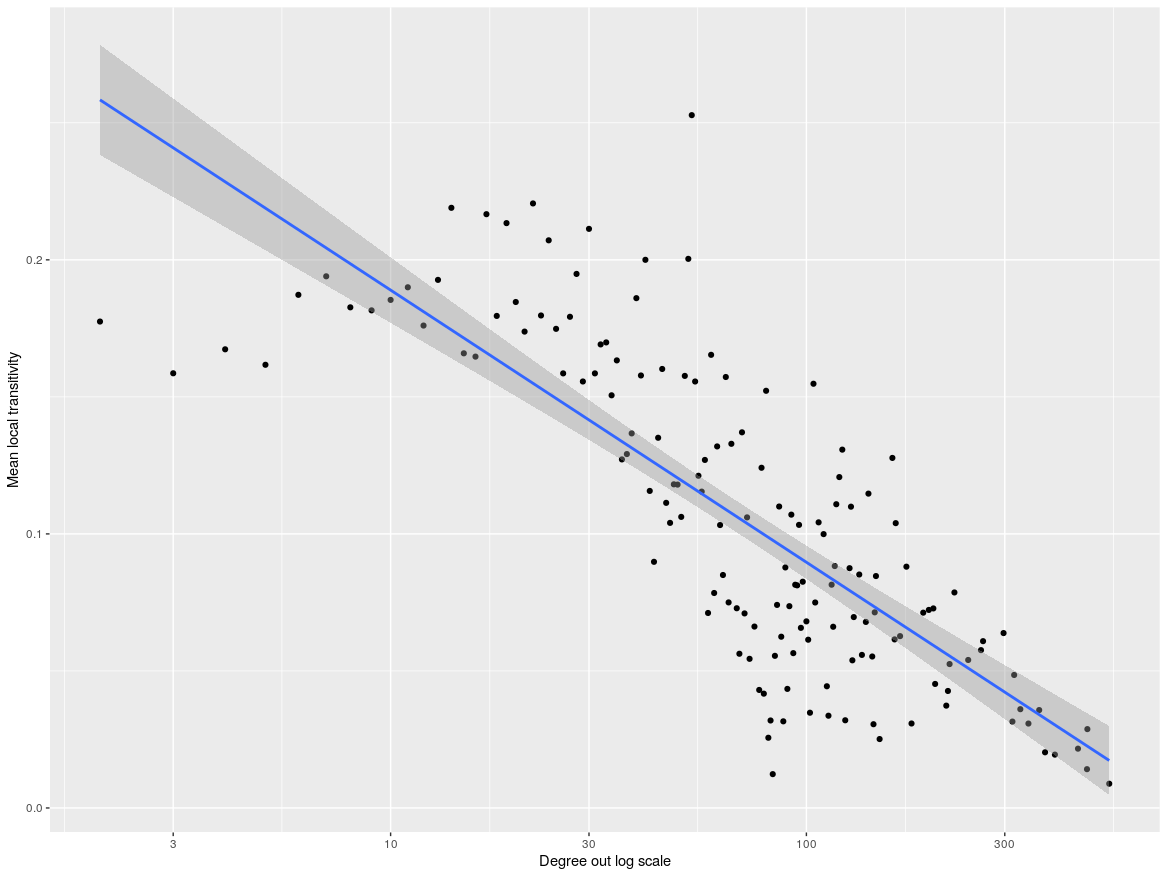
\includegraphics[width=\textwidth]{images/Rplot_k(c)_remove0.png}
    \caption{Plot of degree $k$ log 10 scale with $C(k)$ where $C(k)$ is the mean local undirected transitivity at degree $k$. The point of degree 1 has been removed from the plot and the linear fit as by definition C(k) is 0 as all nodes of degree 1 have local tranisitivity 0 or it is not defined (ie they are isolates) \textcolor{red}{? is this a log-normal distribution seems to be bending down from horizontal at low x. See also graph in Albert Potential replacement can't find original this is not a log scale in transitivity  \url{source('~/RProjects/chapter3/R/transitivity/transitivity_and_degree/mean_deg_seq.R')}}}
    \label{fig:C(k)_remove0}
\end{figure}

% \subsubsection{Panther}
% Panther (Protein ANalysis THrough Evolutionary Relationships) classification system version 15.0 over representation analysis was used.
% \cite{mi2019protocol}
\subsection{Copies of reformatted table}
\subsubsection{DEG}

\begin{table}[]
    \centering
    \begin{tabular}{l|ll}
  
         &      Essential &Not Essential\\
         \hline
PSP      &   2328     &     1129\\
not PSP    &  6616      &    9371   \\

    
    \end{tabular}
    \caption{Contingency table for essential genes. Fisher's exact test p$<2.2\times10^{-16}$. 95\% CI 2.70-3.16 OR 2.92 \url{source('~/RProjects/db_essential_genes/R/get_essential_genes/Fishers_test/fishers test.R')} }
    \label{tab:my_label}
\end{table}


\begin{table}
\pgfplotstabletypeset[
  every head row/.style={%
    before row={\toprule 
        & \multicolumn{2}{c}{Essential}\\            \cmidrule{2-3}},
    after row=\midrule},
  every last row/.style={after row=\bottomrule},
  columns/PSP/.style={string type},
]{
    PSP             Essential Non-essential {Total by PSP}
    PSP                       2328           1112               3440
    NonPSP                     6620           9373               15987
    {Total by Essential}  8992        10509              19427
}
\caption{A caption - update}
\end{table}




\pgfplotstabletypeset[
  every head row/.style={%
    before row={\toprule 
        & \multicolumn{2}{c}{Essential}\\            \cmidrule{2-3}},
    after row=\midrule},
  every last row/.style={after row=\bottomrule},
  columns/PSP/.style={string type},
]{
    PSP             Essential Non-essential {Total by PSP}
    PSP                       2328           1112               3440
    NonPSP                     6614           9373               15987
    {Total by Essential}  8942          10509              19427
}

\subsection{Removed tables}
\subsubsection{DEG - reformatted}
% latex table generated in R 3.6.3 by xtable 1.8-4 package
% Sat Feb 27 14:47:18 2021
\begin{table}[ht]
\centering
\begin{tabular}{lrrrr}
  \hline
Study & Odds ratio & 95\% CI Lower & 95\%CI Upper & p \\ 
  \hline
Any DEG vs none & 2.879 & 2.663 & 3.115 & $1.968 \times 10^{-166}$ \\ 
  Greater than 5 DEG v none & 2.671 & 2.418 & 2.949 & $6.162 \times 10^{-79}$ \\ 
   \hline
\end{tabular}
\caption{Fishers exact test for over representation of synaptic genes in DEG (database of essential genes). First is any appearance in DEG vs genes not in DEG. Second is those in five or more (see methods)}
\tiny\url{source('~/RProjects/db_essential_genes/R/get_essential_genes/db_2020/findforfive/get_db_essential_greater_five_results_xtable.R')}
\end{table}
   % latex table generated in R 3.6.3 by xtable 1.8-4 package
% Sat Feb 27 14:28:09 2021
\begin{table}[ht]
\centering
\begin{tabular}{lrr}
  \hline
 & Synaptic & NonSynaptic \\ 
  \hline
Essential & 2328 & 6664 \\ 
  NonEssential & 1129 & 9306 \\ 
   \hline
\end{tabular}
    `\caption{Database of essential genes. Genes appearing in any entry.\url{source('~/RProjects/db_essential_genes/R/get_essential_genes/db_2020/findforfive/get_db_essential_greater_five_results_xtable.R')}} 
\end{table}

\begin{table}[ht]
\centering
\begin{tabular}{lrr}
  \hline
 & Essential & NonEssential \\ 
  \hline
Synaptic & 2328 & 1129 \\ 
  NonSynaptic & 6664 & 9306 \\ 
   \hline
\end{tabular}
\caption{Database of essential genes. Genes appearing in any entry\url{source('~/RProjects/db_essential_genes/R/get_essential_genes/db_2020/findforfive/get_db_essential_greater_five_results_xtable_transpose.R')}} 
\end{table}
% latex table generated in R 3.6.3 by xtable 1.8-4 package
% Sat Feb 27 14:28:09 2021
\begin{table}[ht]
\centering
\begin{tabular}{lrr}
  \hline
 & Synaptic & NonSynaptic \\ 
  \hline
Essential5 & 728 & 1450 \\ 
  NonEssential & 2729 & 14520 \\ 
   \hline
\end{tabular}
\caption{Database of essential genes. Genes appearing in 5 or more experiments\url{source('~/RProjects/db_essential_genes/R/get_essential_genes/db_2020/findforfive/get_db_essential_greater_five_results_xtable.R')}} 
\end{table} 


\subsubsection{DEG - previous data}
\begin{table}
\centering
\begin{tabular}{cccc}
\toprule
& \multicolumn{2}{c}{Essential} & \\
\cmidrule{2-3}
    PSP & Essential &  Non-Essential & Total by PSP\vspace{1mm} \\
\midrule 
PSP      &   2,328     &     1,129 & 3,457\vspace{1mm}\\
not PSP    &  6,616      &    9,371  & 15,987\vspace{1mm}\\
\midrule
 Total by essential & 8944 & 10050 &  \\ 

 
\bottomrule
\end{tabular}
\caption{Contingency table showing essential genes where essentialness is appearing once in the Database of Essential Genes (DEG). Total genes (19444).  Fisher's exact test p$<2.2\times10^{-16}$. 95\% CI 2.70-3.16; OR 2.92. This may be previous table do for new table below \url{source('~/RProjects/db_essential_genes/R/get_essential_genes/Fishers_test/fishers test.R')}}
\end{table}
\subsubsection{Assortativity}
\begin{table}[ht]
\centering
\begin{tabular}{lrrrrrr}
  \toprule
name & Min. & 1st Qu. & Median & Mean & 3rd Qu. & Max. \\ 
  \midrule
Education Discovery & -0.023 & -0.005 & -0.001 & -0.001 & 0.002 & 0.019 \\ 
  Education Replication & -0.024 & -0.005 & -0.001 & -0.001 & 0.002 & 0.019 \\ 
  Intelligence Discovery & -0.028 & -0.005 & -0.001 & -0.001 & 0.002 & 0.018 \\ 
  Intelligence Replication & -0.023 & -0.005 & -0.001 & -0.001 & 0.002 & 0.022 \\ 
   \bottomrule
\end{tabular}
\caption{Bootstrap estimate of null model parameters Assortativity by z score}
\label{tab:Bootstrap estimate of null model parameters Assortativity by z score}
\end{table}


\begin{table}[]
     \centering
     \begin{tabular}{llll}
     \toprule
         Study & Missing values  & Assortativity\textsubscript{0} & Assortativity\textsubscript{median}\\
         \midrule
         Intelligence\textsubscript{Replication} & 148 & 0.003 & 0.0032\\
         Education\textsubscript{Replication} & 172 & -0.006 &  -0.0064\\
         Education\textsubscript{Discovery} & 156 & 0.001 & -0.0002\\
         Intelligence\textsubscript{Discovery} & 156 & -0.004 & -0.0038\\
         \bottomrule
     \end{tabular}
     \caption{Assortativity of PSP graph vertices by study Z score. PSP graph members without corresponding Z score marked as missing values had z set to either 0 (Assortativity\textsubscript{0} or the median z score Assortativity\textsubscript{median}\url{source('~/RProjects/chapter3/R/assortativity_distribution/z_score/assortativity_z.R', echo=TRUE)} for missing set to zero \url{source('~/RProjects/centrality/R/get_gene_scores/assortativity_with_z_scores.R')} . All values not significantly different ($p>0.05$) than bootstrap estimate of assortativity (\url{source('~/RProjects/chapter3/R/assortativity_distribution/bootstrap/bootstrap_zscore_assortativity_studies.R')} }
     \label{tab:Assortativity of PSP graph and z scores}
 \end{table}
 
 
 
\begin{table}[]
     \centering
     \begin{tabular}{ccc}
     \toprule
         Study & Missing values  & Assortativity\\
         \midrule
         Intelligence\textsubscript{Replication} & 148 & 0.003187\\
         Education\textsubscript{Replication} & 172 & -0.006424\\
         Education\textsubscript{Discovery} & 156 & -0.000214\\
         Intelligence\textsubscript{Discovery} & 156 & -0.003780\\
         \bottomrule
     \end{tabular}
     \caption{Assortativity of PSP graph vertices by study Z score. PSP graph members without corresponding Z score marked as missing values had z set to median score. Script\url{source('~/RProjects/chapter3/R/assortativity_distribution/z_score/assortativity_z.R', echo=TRUE)}}
     \label{tab:Assortativity of PSP graph and z scores_impute_median}
 \end{table}
 
 \subsubsection{Summary of centrality measures}
\begin{table}[ht]
\centering
\begin{adjustbox}{width=\textwidth}

\begin{tabular}{lllllll}
  \toprule
 Centrality measure & Minimum & 1st Quartile & Median & Mean & 3rd Quartile & Maximum \\ 
 \midrule
Degree & $1 $ & $4 $ & $8 $ & $17.64$  & $19$ & $535$ \\ 
  Eigenvector & $1.821 \times 10^{-6}$ & $8.829 \times 10^{-3}$ & $2.194 \times 10^{-2}$ & $4.793 \times 10^{-2}$ & $5.322 \times 10^{-2}$ & 1 \\ 
   Betweenness & $0 $ & $43.29 $ & $317 $ & $3421.1$ & $1571.6$& $6.447 \times 10^{5}$ \\ 
  Transitivity NA & 0  & 0.043 & 0.129 & 0.171 & 0.238 & $1 $ \\ 
  Transitivitiy 0 & 0  & 0 & 0.108  & 0.156  & 0.223  & $1$ \\ 
  Closeness & $5.702 \times 10^{-5}$ & $9.217 \times 10^{-5}$ & $9.879 \times 10^{-5}$ & $9.845 \times 10^{-5}$ & $1.058 \times 10^{-4}$ & $1.399 \times 10^{-4}$ \\ 
  k-core & 1 & 3 & 8 & 9.15 & 13& 24 \\ 
   \bottomrule
\end{tabular}
\end{adjustbox}
\caption{Summary of results of centrality measures. Transitivity NA records isolates (nodes with degree 1) as having an undefined transitivity and they are removed before calculating the summary statistics. Transitivity 0 uses the alternate method of assigning isolates a transitivity of 0} 
\label{Table:Summary of centrality measures}
\end{table}

% Annotation version PANTHER Data at a glance: Version 15.0 released 2020-02-14. Gene (Reference Proteome 2019\_04 release)

  % latex table generated in R 3.6.3 by xtable 1.8-4 package
% Tue Nov 10 17:16:04 2020
\begin{table}[ht]
\centering
\begin{tabular}{rrrrrrr}
  \toprule
 & Degree & Betweenness & Eigenvector & Closeness & Transitivity & kcoreness \\ 
  \midrule
Min. & 1.0 & 0.0 & $1.82 \times 10^{-6}$ & $5.702 \times 10^{-5}$ & 0.000 & 1.0 \\ 
  1st Qu. & 4.0 & 43.3 & $8.83 \times 10^{-3}$ & $9.217 \times 10^{-5}$ & 0.000 & 3.0 \\ 
  Median & 8.0 & 317.0 & $2.19 \times 10^{-2}$ & $9.879 \times 10^{-5}$ & 0.108 & 8.0 \\ 
  Mean & 17.6 & 3421.1 & $4.79 \times 10^{-2}$ & $9.845 \times 10^{-5}$ & 0.156 & 9.2 \\ 
  3rd Qu. & 19.0 & 1571.6 & $5.32 \times 10^{-2}$ & $1.058 \times 10^{-4}$ & 0.221 & 13.0 \\ 
  Max. & 535.0 & 644670.7 & $1.00 \times 10^{0}$ & $1.399 \times 10^{-4}$ & 1.000 & 24.0 \\ 
   \bottomrule
\end{tabular}
\caption{Transpose of summary table source is \url{source('~/RProjects/chapter3/R/centrality_ch3/summary_centrality.R')}}
\end{table}


% %  Family (PANTHER™ 15.0, released 2020-02-14)

   


% %  Pathways

% %     PANTHER™ Pathway 3.6.4, released 2020-02-14
% %         177 pathways
% %         3092 pathway components
% %         53228 sequence associated to pathways
% %         6000 references captured for the pathways

% %     Reactome (from Reactome database version 65, released 2019-12-22)
% %         21535 total terms


% %  Ontologies

% %     PANTHER™ GO slim (version 15.0, based on GO release 2018-07-03, released 2020-02-14)
% %         3219 total terms
% %         2137 biological process terms
% %         548 cellular component terms
% %         534 molecular function terms
% %     PANTHER™ Protein Class (version 15.0, released 2020-02-14)
% %         210 total terms


% %     Gene Ontology (from GO database released 2020-06-01, DOI: 10.5281/zenodo.3873405)
% %         47228 total terms
% %         12038 molecular function terms
% %         30818 biological process terms
% %         4372 cellular component terms


%     Analysis Type -  PANTHER Overrepresentation Test (Released 20200407)
    
%     Annotation Version and Release Date -  Reactome version 65 Released 2019-12-22
%                                             Panther GO SLIM  PANTHER version 15.0 Released 2020-02-14
%                                             Panther pathways PANTHER version 15.0 Released 2020-02-14
%                                             Panther Protein class  Panther pathways PANTHER version 15.0 Released 2020-02-14
%                                             GO  GO Ontology database DOI: 10.5281/zenodo.3873405 Released 2020-06-01
 
%     Analyzed List - The genes representing extreme values of centrality measures in this case 0.9 and 0.1 centile. The size of group may be greater than 345 as some centrality measures had more genes with their maximal or minimal value than 3457
    
%     Reference List - The reference gene list for the test. The reference list is the genes in the PSP (n=3457) or the default panther set \todo{or those in one study}
    
%     Annotation Data Set 
%         PANTHER Pathway
%         PANTHER GO-slim Molecular Function
%         PANTHER GO-slim Biological Process
%         PANTHER GO-slim Cellular Component
%         PANTHER Protein Class
%         GO molecular function complete - Complete GO molecular function annotations including both manually curated and electronic annotations. Electronic annotations are generated by computer algorithm based on sequence similarity, and are usually not reviewed by curators. They are less reliable.
%         GO biological process complete 
%         GO cellular component complete 
%         Reactome Pathway
        
%     Test Type - Fisher's exact test with FDR correction




% \todo{background}
% \todo{Fishers test}
% \todo{topgo}


% \subsection{Methods GO Slim}
% \textcolor{red}{Define}

\subsection{Murine centrality}
\subsubsection{t tests}



\begin{table}[ht]
\centering
\begin{adjustbox}{width=\textwidth}

\begin{tabular}{lrrrrrrrrr}
  \toprule
 & t & df & low & high & $\mu_x$ & $mu_y$ & stderr & $p$ & p\_BH \\ 
  \midrule
abnormal spatial learning & 0.799 & 129.936 & $-1.143 \times 10^{-6}$ & $2.691 \times 10^{-6}$ & $9.923 \times 10^{-5}$ & $9.845 \times 10^{-5}$ & $9.691 \times 10^{-7}$ & 0.426 & 0.838 \\ 
  abnormal temporal memory & 0.026 & 112.210 & $-2.233 \times 10^{-6}$ & $2.294 \times 10^{-6}$ & $9.848 \times 10^{-5}$ & $9.845 \times 10^{-5}$ & $1.142 \times 10^{-6}$ & 0.979 & 0.979 \\ 
  abn context condition & -0.546 & 99.075 & $-3.006 \times 10^{-6}$ & $1.709 \times 10^{-6}$ & $9.780 \times 10^{-5}$ & $9.845 \times 10^{-5}$ & $1.188 \times 10^{-6}$ & 0.587 & 0.838 \\ 
  reduced long term potentiation & -1.302 & 104.153 & $-3.973 \times 10^{-6}$ & $8.231 \times 10^{-7}$ & $9.688 \times 10^{-5}$ & $9.845 \times 10^{-5}$ & $1.209 \times 10^{-6}$ & 0.196 & 0.652 \\ 
  abnormal LTDep & -3.343 & 67.791 & $-7.086 \times 10^{-6}$ & $-1.789 \times 10^{-6}$ & $9.402 \times 10^{-5}$ & $9.845 \times 10^{-5}$ & $1.327 \times 10^{-6}$ & 0.001 & 0.014 \\ 
  abn assoc learning & -0.587 & 163.224 & $-2.322 \times 10^{-6}$ & $1.257 \times 10^{-6}$ & $9.792 \times 10^{-5}$ & $9.845 \times 10^{-5}$ & $9.064 \times 10^{-7}$ & 0.558 & 0.838 \\ 
  abormal associative learning & -0.587 & 163.224 & $-2.322 \times 10^{-6}$ & $1.257 \times 10^{-6}$ & $9.792 \times 10^{-5}$ & $9.845 \times 10^{-5}$ & $9.064 \times 10^{-7}$ & 0.558 & 0.838 \\ 
  abnormal learning memory conditioning & -0.117 & 360.689 & $-1.378 \times 10^{-6}$ & $1.223 \times 10^{-6}$ & $9.838 \times 10^{-5}$ & $9.845 \times 10^{-5}$ & $6.613 \times 10^{-7}$ & 0.907 & 0.979 \\ 
  abnormal synaptic plasticity & -2.507 & 50.663 & $-6.718 \times 10^{-6}$ & $-7.428 \times 10^{-7}$ & $9.472 \times 10^{-5}$ & $9.845 \times 10^{-5}$ & $1.488 \times 10^{-6}$ & 0.015 & 0.077 \\ 
  abnormal cognition & -0.117 & 360.689 & $-1.378 \times 10^{-6}$ & $1.223 \times 10^{-6}$ & $9.838 \times 10^{-5}$ & $9.845 \times 10^{-5}$ & $6.613 \times 10^{-7}$ & 0.907 & 0.979 \\ 
   \bottomrule
\end{tabular}
\end{adjustbox}
\caption{Closeness centrality t test versus PSP. p adjust with BH}
\tiny\url{source('~/RProjects/chapter3/R/murine_centrality/general_murine_boxplot/rough_centrality_boxplot_murine_ltp_general_closeness_add_table.R'}

\end{table}

\begin{table}[ht]
\centering
\begin{tabular}{rrrrrrrrrr}
  \toprule
 & t & df & low & high & mean\_x & mean\_y & stderr & p & p\_BH \\ 
  \midrule
abnormal spatial learning & 1.001 & 121.019 & $-5.256 \times 10^{3}$ & $1.601 \times 10^{4}$ & $8.799 \times 10^{3}$ & $3.421 \times 10^{3}$ & $5.371 \times 10^{3}$ & 0.319 & 0.406 \\ 
  abnormal temporal memory & 1.117 & 106.680 & $-5.347 \times 10^{3}$ & $1.914 \times 10^{4}$ & $1.032 \times 10^{4}$ & $3.421 \times 10^{3}$ & $6.175 \times 10^{3}$ & 0.267 & 0.406 \\ 
  abn context condition & 0.962 & 94.493 & $-6.984 \times 10^{3}$ & $2.011 \times 10^{4}$ & $9.983 \times 10^{3}$ & $3.421 \times 10^{3}$ & $6.822 \times 10^{3}$ & 0.339 & 0.406 \\ 
  reduced long term potentiation & 0.942 & 99.575 & $-6.759 \times 10^{3}$ & $1.898 \times 10^{4}$ & $9.533 \times 10^{3}$ & $3.421 \times 10^{3}$ & $6.487 \times 10^{3}$ & 0.348 & 0.406 \\ 
  abnormal LTDep & -2.746 & 134.891 & $-2.973 \times 10^{3}$ & $-4.836 \times 10^{2}$ & $1.693 \times 10^{3}$ & $3.421 \times 10^{3}$ & $6.295 \times 10^{2}$ & 0.007 & 0.075 \\ 
  abn assoc learning & 0.986 & 150.935 & $-4.306 \times 10^{3}$ & $1.288 \times 10^{4}$ & $7.708 \times 10^{3}$ & $3.421 \times 10^{3}$ & $4.349 \times 10^{3}$ & 0.326 & 0.406 \\ 
  abnormal associative learning & 0.986 & 150.935 & $-4.306 \times 10^{3}$ & $1.288 \times 10^{4}$ & $7.708 \times 10^{3}$ & $3.421 \times 10^{3}$ & $4.349 \times 10^{3}$ & 0.326 & 0.406 \\ 
  abnormal learning memory conditioning & 1.056 & 318.355 & $-2.033 \times 10^{3}$ & $6.747 \times 10^{3}$ & $5.778 \times 10^{3}$ & $3.421 \times 10^{3}$ & $2.231 \times 10^{3}$ & 0.292 & 0.406 \\ 
  abnormal LTP & 0.902 & 142.647 & $-4.928 \times 10^{3}$ & $1.319 \times 10^{4}$ & $7.555 \times 10^{3}$ & $3.421 \times 10^{3}$ & $4.584 \times 10^{3}$ & 0.369 & 0.406 \\ 
  abnormal synaptic plasticity & -0.517 & 61.216 & $-2.703 \times 10^{3}$ & $1.593 \times 10^{3}$ & $2.866 \times 10^{3}$ & $3.421 \times 10^{3}$ & $1.074 \times 10^{3}$ & 0.607 & 0.607 \\ 
  abnormal cognition & 1.056 & 318.355 & $-2.033 \times 10^{3}$ & $6.747 \times 10^{3}$ & $5.778 \times 10^{3}$ & $3.421 \times 10^{3}$ & $2.231 \times 10^{3}$ & 0.292 & 0.406 \\ 
   \bottomrule
\end{tabular}
\caption{Betweenness centrality murine}
\end{table}
\paragraph{From introduction}
\subparagraph{Removed}\textcolor{red}{? remove following}. The gene duplication event \cite{grant2016molecular} potentially affected network topology through duplication divergence \cite{ispolatov2005duplication}\cite{taylor2004duplication}\cite{wagner2003global}. 
\paragraph{Notes and suggestions}
Also motifs (other than number of triangles) newman 334 again

